\documentclass[a4paper]{scrartcl}
\usepackage[utf8]{inputenc}
\usepackage[english]{babel}

\usepackage{amsmath}
\usepackage{amsfonts} % for mathbb for instance
\usepackage{mathtools}
\usepackage[amsmath, amsthm, framed, thmmarks]{ntheorem}

\usepackage[usenames,dvipsnames,svgnames,table]{xcolor}


% specifics about the pdf
\usepackage[english]{babel}
\usepackage[pdftex]{graphicx}
\usepackage[pdftex,bookmarks,colorlinks,pdffitwindow]{hyperref}

\usepackage{multicol}  
%\usepackage[rflt]{floatflt}  
\usepackage{epsfig} 
%\usepackage{qtree} 
\usepackage{url}

\usepackage{todonotes}

% PDF Import support
\usepackage{pdfpages}
% Support for PDF scaling
\usepackage{graphicx}
% Algorithmen
\usepackage{algorithmic}
\usepackage{algorithm}
\usepackage{listings} 
% \lstset{numbers=left, numberstyle=\tiny, numbersep=5pt} 
\lstset{
	basicstyle=\ttfamily\scriptsize\mdseries,
	keywordstyle=\bfseries\color{blue},
	identifierstyle=,
% 	stringstyle=\itshape\color{red},
	numbers=left,
	numberstyle=\tiny,
	stepnumber=10,
	breaklines=true,
	frame=none,
	showstringspaces=false,
	tabsize=4,
% 	backgroundcolor=\color{gray},
% 	morecomment=[s][\color{green}]{/+}{+/},
	commentstyle=\color{gray},	
	captionpos=b,
	float=htbp,
}
% math packages


% redefine greek letters
\renewcommand{\phi}{\varphi}
\renewcommand{\epsilon}{\varepsilon}

% shortcuts in math mode
\newcommand{\bs}{\boldsymbol}
\newcommand{\mc}{\mathcal}
\newcommand{\ds}{\displaystyle}
\DeclarePairedDelimiter\absimpl{\lvert}{\rvert}
\DeclarePairedDelimiter\normimpl{\lVert}{\rVert}
\newcommand{\abs}[1]{\absimpl*{#1}}
\newcommand{\norm}[1]{\normimpl*{#1}}
\newcommand{\argmax}{\operatorname*{arg\,max}}
\newcommand{\argmin}{\operatorname*{arg\,min}}

% number sets
\newcommand{\R}{\mathbb{R}}
\newcommand{\Z}{\mathbb{Z}}
\newcommand{\N}{\mathbb{N}}
\newcommand{\Q}{\mathbb{Q}}
\newcommand{\C}{\mathbb{C}}
\newcommand{\F}{\mathbb{F}}
\newcommand{\LL}{\mathcal{L}}
\newcommand{\powerset}{\mathcal P}
\newcommand{\normal}{\mathcal N}

% probabilities
\newcommand{\Prob}[1]{\operatorname{Pr}\left[#1\right]}
\newcommand{\Ex}[1]{\mathbb{E}\left[#1\right]}

% misc
\newcommand{\bigO}[1]{\mc O\left(#1\right)} % big-o notation

\newcommand{\nop}[1]{} % temporarily remove from output

\let\oldemph\emph
\renewcommand{\emph}[1]{{\color{red}\oldemph{#1}}}

% remove the paragraph indentation
 \setlength{\parindent}{0in}

\author{Pascal Spörri\\pascal@spoerri.io}
\title{Scientific Visualisation Summary\\ FS 2013\\ }
%\thanks{Licence: Creative Commons Attribution-Share Alike 3.0 Unported (\url{http://creativecommons.org/licenses/by-sa/3.0/})}}
\date{\today}

\begin{document}
\maketitle
This summary is based on the course slides of the Scientific Visualisation course at ETH Zürich\footnote{\url{http://www.scivis.ethz.ch/education/scivis_course/notes}} from spring semester 2013.
\newpage
\tableofcontents
\newpage
\section{Introduction}

SciVis is interdisciplinary the fields of application include engineering, natural sciences and medical sciences.   There's a common application to all fields: 
There are \emph{numerical datasets} providing an abstraction from the particular application. The characteristics of such datasets include:
\begin{description}
\item[Dimension of domain:] Number of coordinates or parameters
\item[Dimension of values:] Scalar, vector or tensor fields
\item[Type of data:] Discrete values versus discretised data
\item[Type of discretisation:] (Un-)structured grid, scattered data
\item[Time dependencies:] Static versus time-dependent.
\end{description}

\subsubsection{SciVis and InfoVis}
\begin{description}
    \item[Scientific Visualisation] is mostly concerned with 
        \begin{itemize}
            \item 2,3,4 dimension spatial or spatio-temporal data
            \item discretised data
        \end{itemize}
    \item[Information Visualisation] focuses on:
        \begin{itemize}
            \item High-dimensional, abstract data
            \item Discrete data
            \item Financial, statistical, etc.
            \item Visualisation of large trees, networks, graphs
            \item Data mining:
                \begin{itemize}
                    \item Finding patterns
                    \item Clusters
                    \item Voids
                    \item Outliers
                \end{itemize}
                
        \end{itemize}

\end{description}

\subsection{Visualisation Scenarios}
The reference model for visualisation:
\begin{figure}[H]
    \centering
    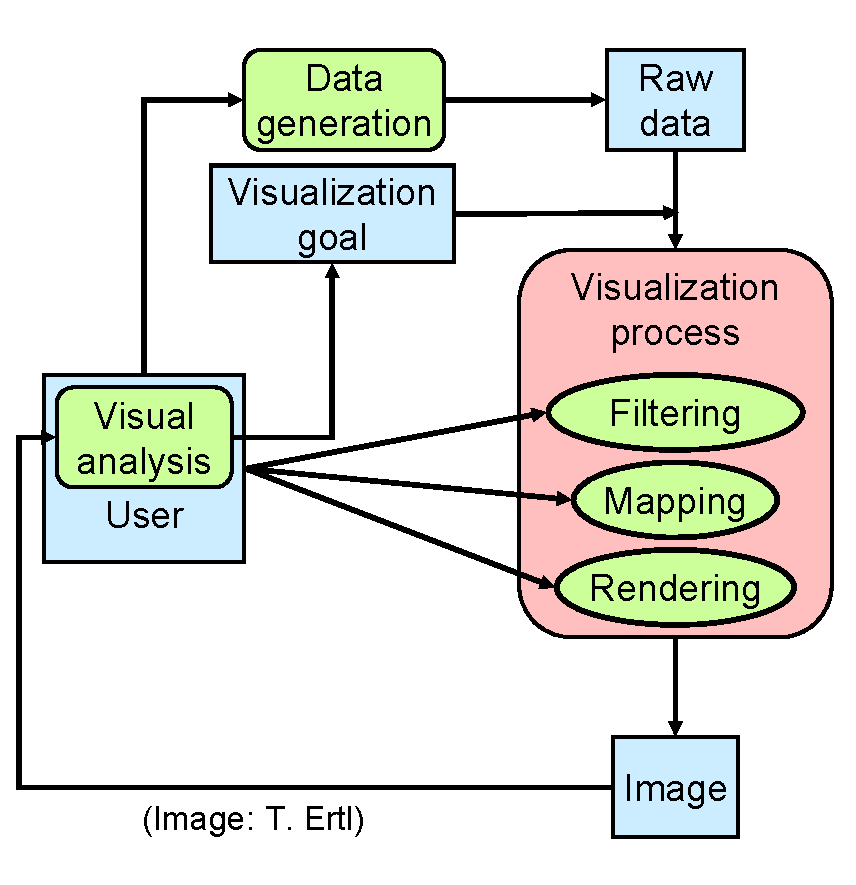
\includegraphics[width=0.5\textwidth]{img/01_vis_scenarios}
\end{figure}
\subsubsection{Video/Movie}
In a first step the data is generated. Then the data is visualised during a batch visualisation step and in the end the video is analized. 
\begin{figure}[H]
    \centering
    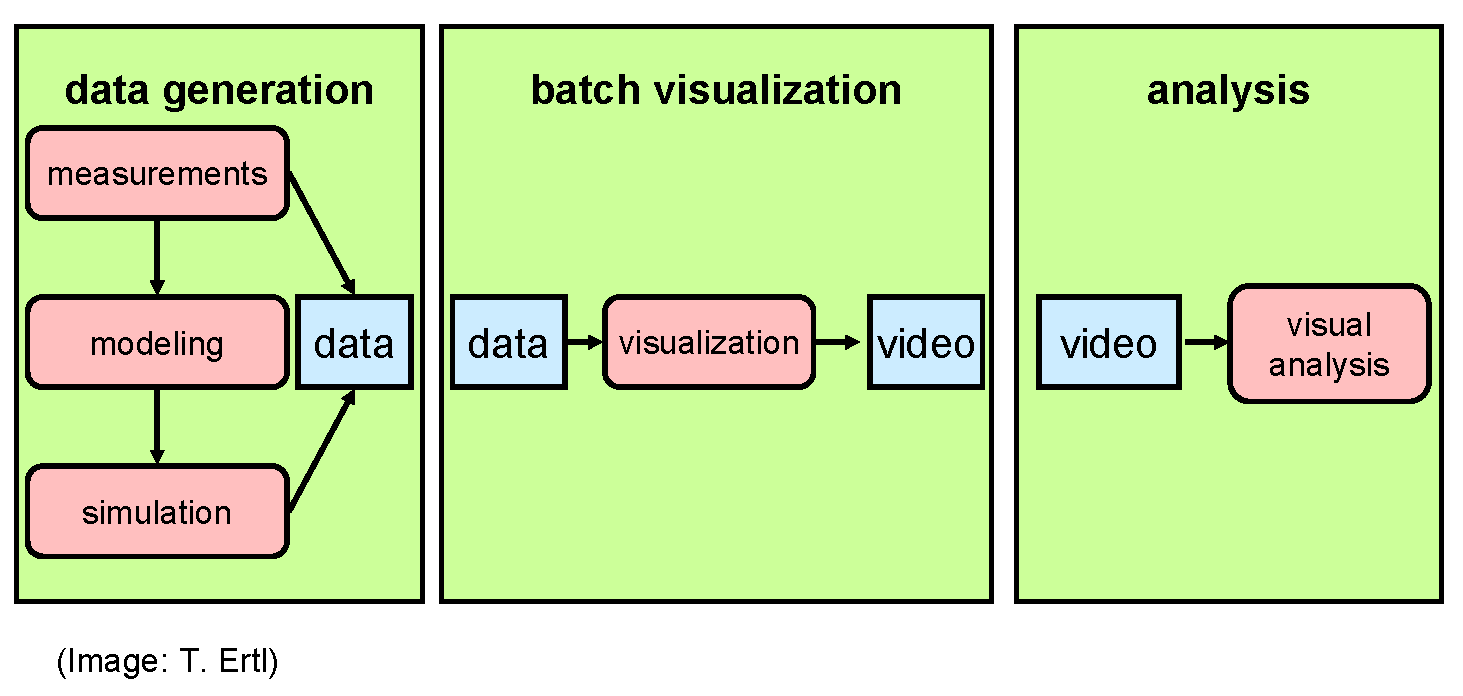
\includegraphics[width=0.75\textwidth]{img/01_movie_mode}
\end{figure}

\subsubsection{Tracking}
The gathered data is directly visualised and analysed.
\begin{figure}[H]
    \centering
    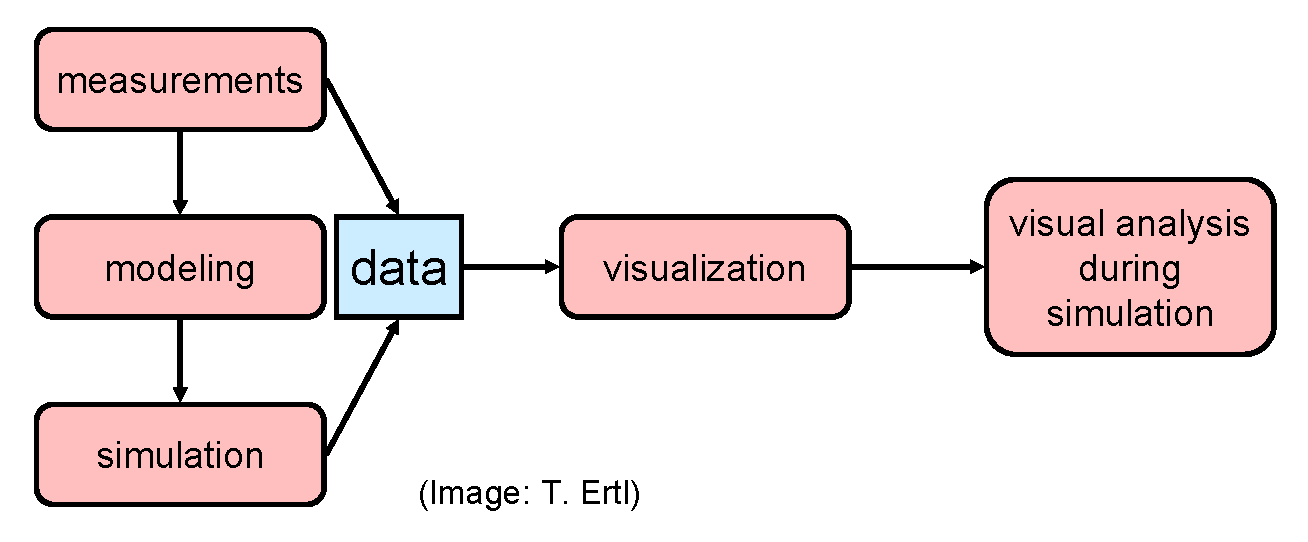
\includegraphics[width=0.75\textwidth]{img/01_tracking}
\end{figure}
\subsubsection{Interactive Post Processing/Visualisation}
The data generation step is split from the visualisation step. 
\begin{figure}[H]
    \centering
    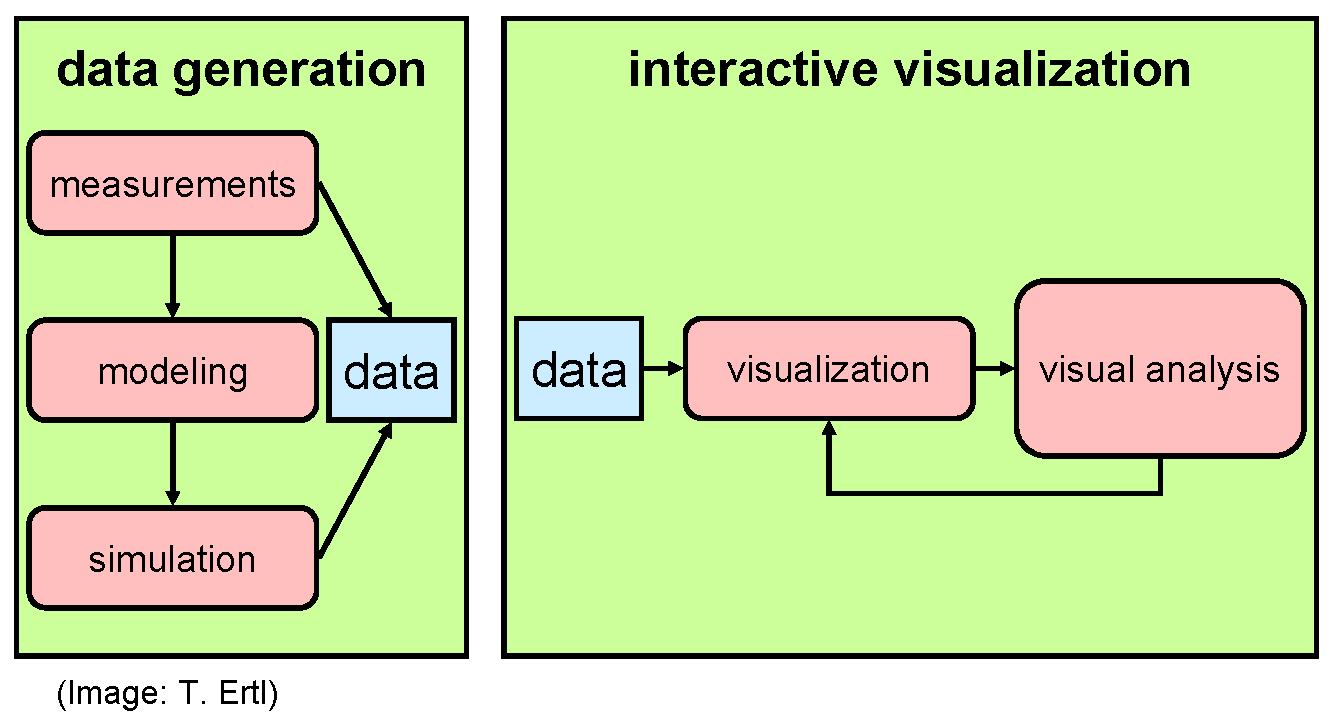
\includegraphics[width=0.75\textwidth]{img/01_interactive_post}
\end{figure}
\subsubsection{Interactive Steering/Computational Steering}
The visualisation has a direct impact on the simulation and the visualisation.
\begin{figure}[H]
    \centering
    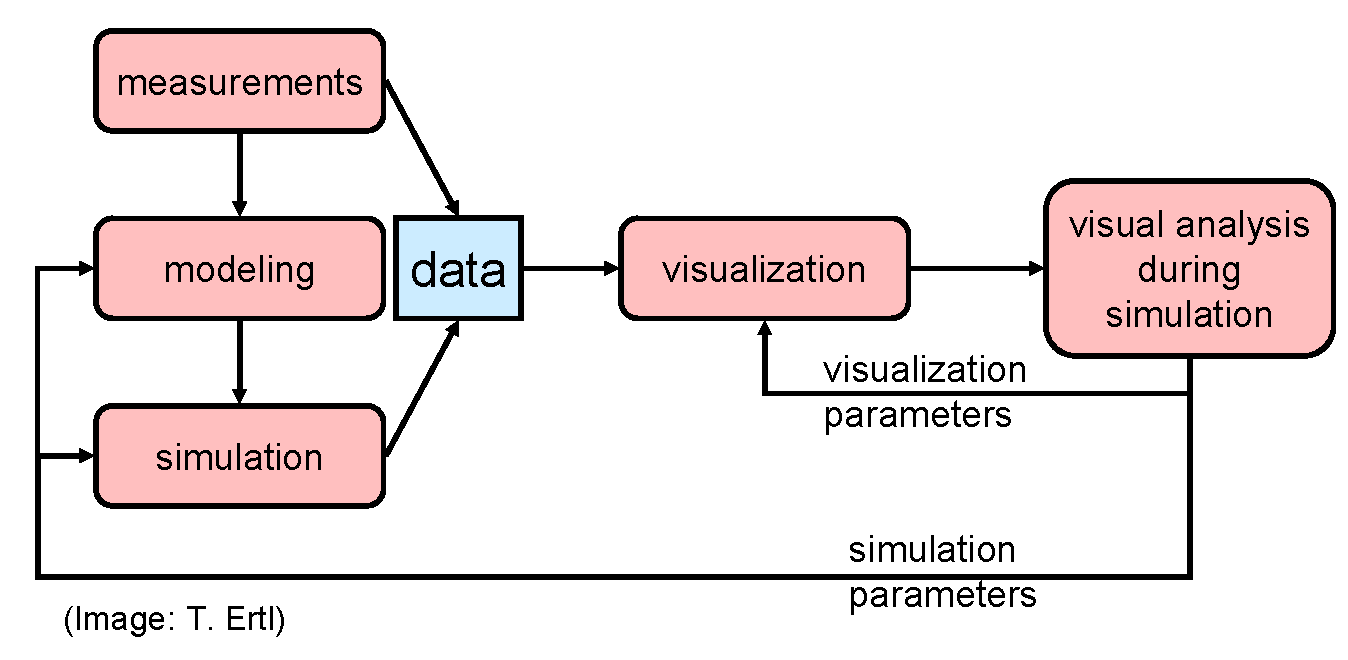
\includegraphics[width=0.75\textwidth]{img/01_interactive_steering}
\end{figure}

\subsection{Data Discretisations}
Types of data sources have typical types of discretisations:
\begin{description}
\item[Measurment Data] Typically scattered ("mesh-less", no grid)
\item[Numerical Simulation Data] $\ $
    \begin{itemize}
        \item Structured, block-structured or unstructured grids
        \item Adaptively refined meshes
        \item Multi-Zone grids with relative motion
        \item ...
    \end{itemize}
\item[Imaging Methods] Uniform grids
\item[Mathematical Functions] (and functionally represented data) can be sampled by demand:
    \begin{itemize}
        \item Uniform
        \item Adaptive
    \end{itemize}
\end{description}

\subsection{Unstructured Grids}
\subsubsection{2D Unstructured Grids}
Cells are \emph{triangles} and/por quadrangles. The domain can be a surface embedded in $3$-space (distinguish $n$-dimensional from $n$-space).
\begin{figure}[H]
\centering   
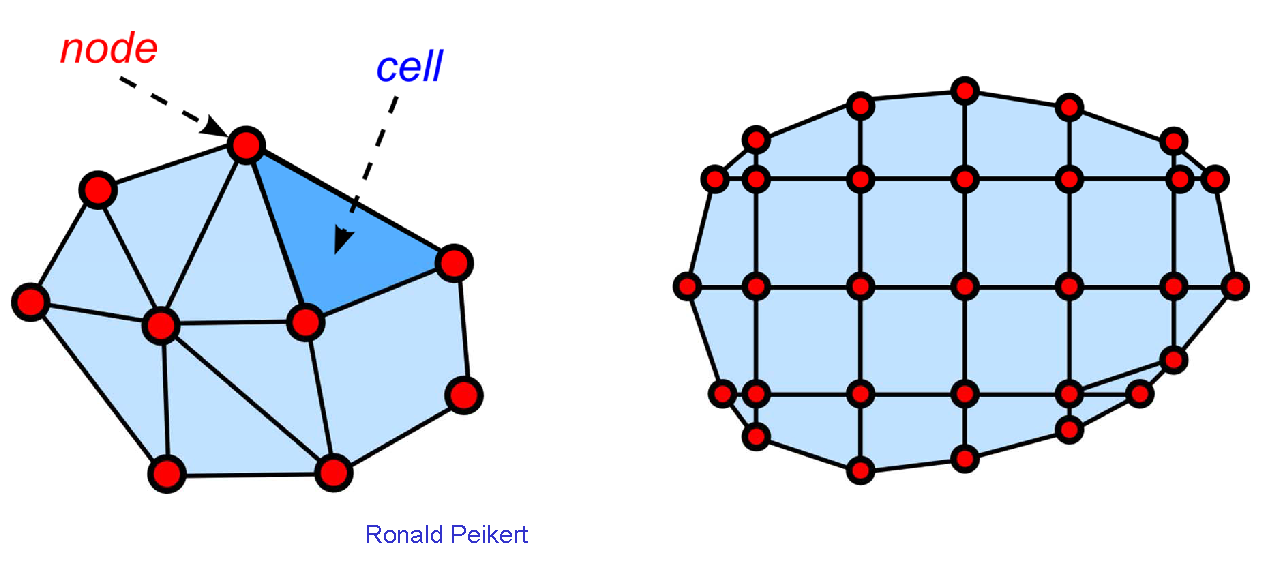
\includegraphics[width=0.75\textwidth]{img/01_unstructured_grids}
\end{figure}

\subsubsection{3D Unstructured Grids}
Cells are \emph{tetrahedra} or \emph{hexahedra}.
\begin{figure}[H]
\centering
\includegraphics[width=0.6\textwidth,page=2]{img/01_3d_unstructured_grids}
\end{figure}
Mixed grids ("zoo meshes") require additional types:
\emph{wedge} ($3$ sided prism), and a \emph{pyramid} ($4$-sided).
\begin{figure}[H]
\centering
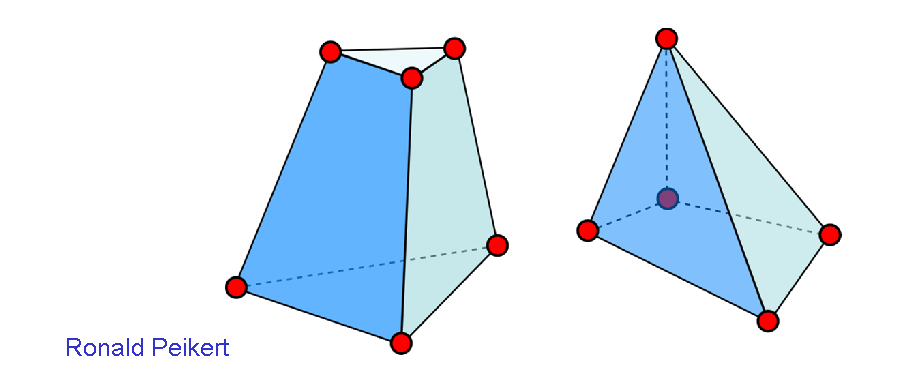
\includegraphics[width=0.6\textwidth,page=1]{img/01_3d_unstructured_grids}
\end{figure}

\subsection{Structured Grids}
\begin{description}
    \item[Curvilinear Grid (general case)] Nodes are given in an array $N_i\times N_j\times N_k$ and the cells are implicit.
    \begin{figure}[H]
        \centering
        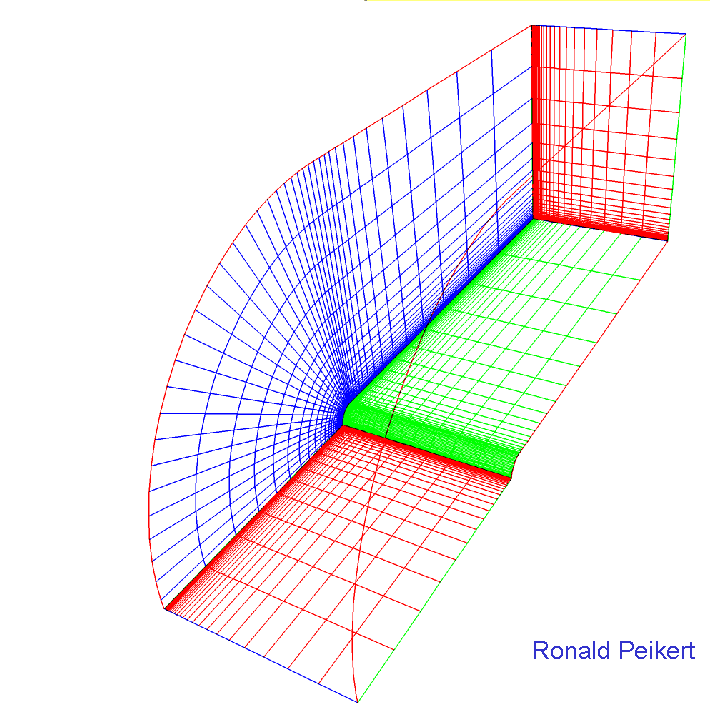
\includegraphics[width=0.5\textwidth]{img/01_curvilinear_grid}
        \caption{Curvilinear Grid}
    \end{figure}

    \item[Rectilinear Grid (special case)] The coordinate functions are simpler:
        \begin{align*}
            x = x(i)\qquad
            y = y(j)\qquad
            z = z(k)
        \end{align*}
        \begin{figure}[H]
            \centering
            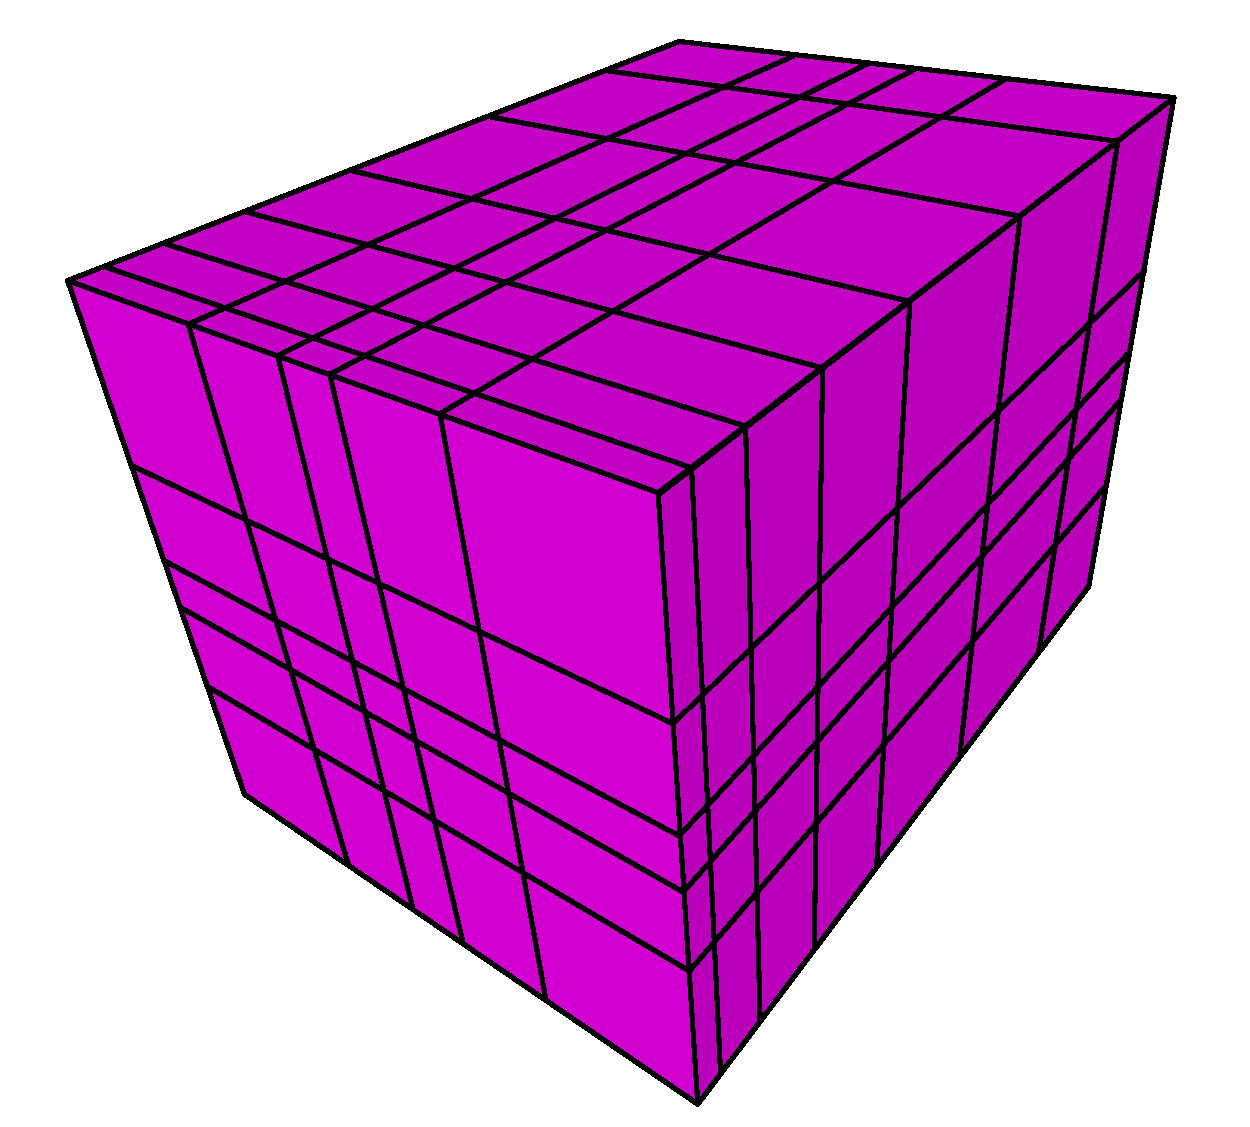
\includegraphics[width=0.25\textwidth]{img/01_rectilinear_grid_wikipedia}
            \caption{Rectilinear Grid, Source: Wikipedia}
        \end{figure}

     \item[Uniform Grid (more special)] The coordinates are defined by an \emph{axis-aligned}bounding box.
\end{description}

\subsubsection{Point-Sampled Data/Scattered Data}
Point sampled data  returns only nodes and no cells. Typical data sources are measurement data for example meteorological data.

Options for visualisation include:
\begin{description}
\item[Point-Based Methods] (relatively few algorithms)
\item[Triangulation] for example constrained Delaunay (difficult in 3D)
\item[Resampling] onto uniform grid.
\end{description}

\subsection{Elementary Visualisation Methods}
\emph{Scalar Fields} can be visualised by plotting its \emph{function graphs}:
\begin{description}
    \item[1D Field:] The Graph is a curve:
        \begin{align*}
            y = f(x)
        \end{align*}
    \item[2D Field:] The Graph is a \emph{height field}:
        \begin{align*}
            z = f(x,y)
        \end{align*}
        Visualisation is easy for rectilinear grids:\\
        \emph{Painter's algorithm} (hidden surface removal in software): Draw cells row by row from back to front.
        \begin{figure}[H]
            \centering
            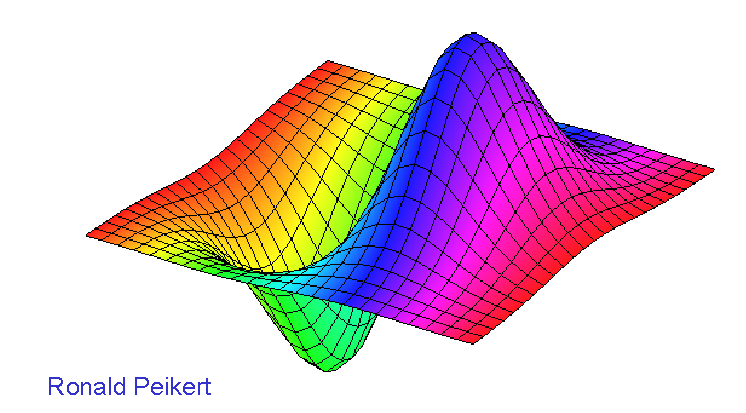
\includegraphics[width=0.7\textwidth]{img/01_painters_algorithm}
        \end{figure}
\end{description}

Scalar fields can also be visualised using \emph{color coding} using \emph{1D texture mapping}. Don't use \emph{vertex colors} and Gouraud shading!
\begin{figure}[H]
    \centering
    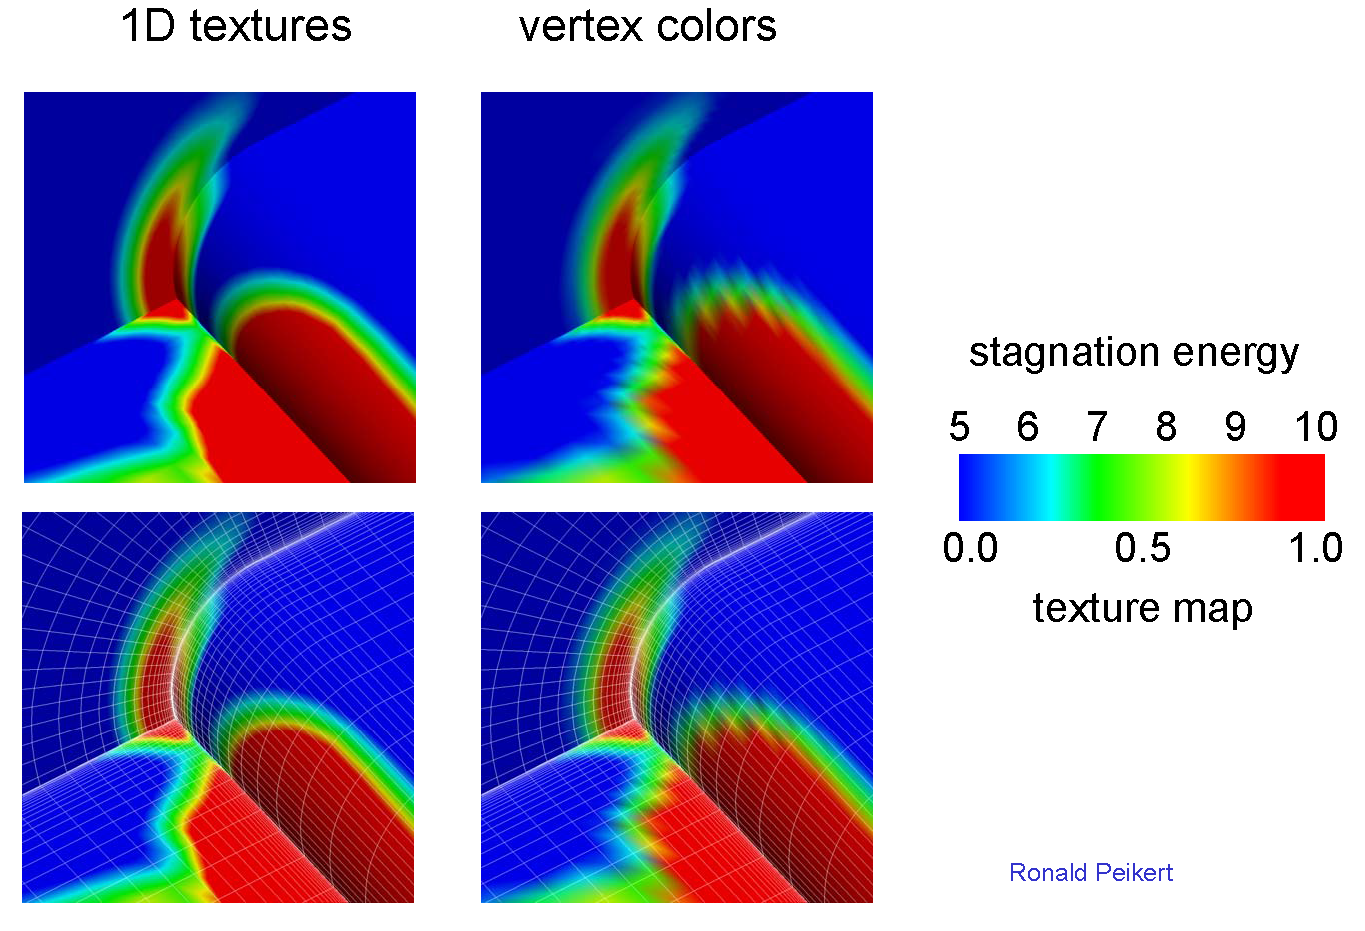
\includegraphics[width=0.9\textwidth]{img/01_texture_mapping}
\end{figure}

\begin{itemize}
    \item Problem of RGB colouring mode: The Interpolation is in the wrong colour space (RGB vs. colour table).
    \item  Problem of Colour Index mode: Lighting is not possible. 
\end{itemize}



\newpage
\section{Contouring and Isosurfaces}

\subsection{Contours}
Contours are a set of points where the scalar field $s$ has a given value $c$:
\begin{align*}
    \left\{ x\in \R^n: s(x) = c\right\}
\end{align*}

Examples in 2D:
\begin{itemize}
    \item Height contours on maps
    \item Isobars on weathermaps
\end{itemize}

\paragraph{Contouring algorithm:}
\begin{itemize}
    \item Find intersection with grid edges
    \item Connect points in each cell
\end{itemize}

\begin{figure}[H]
    \centering
    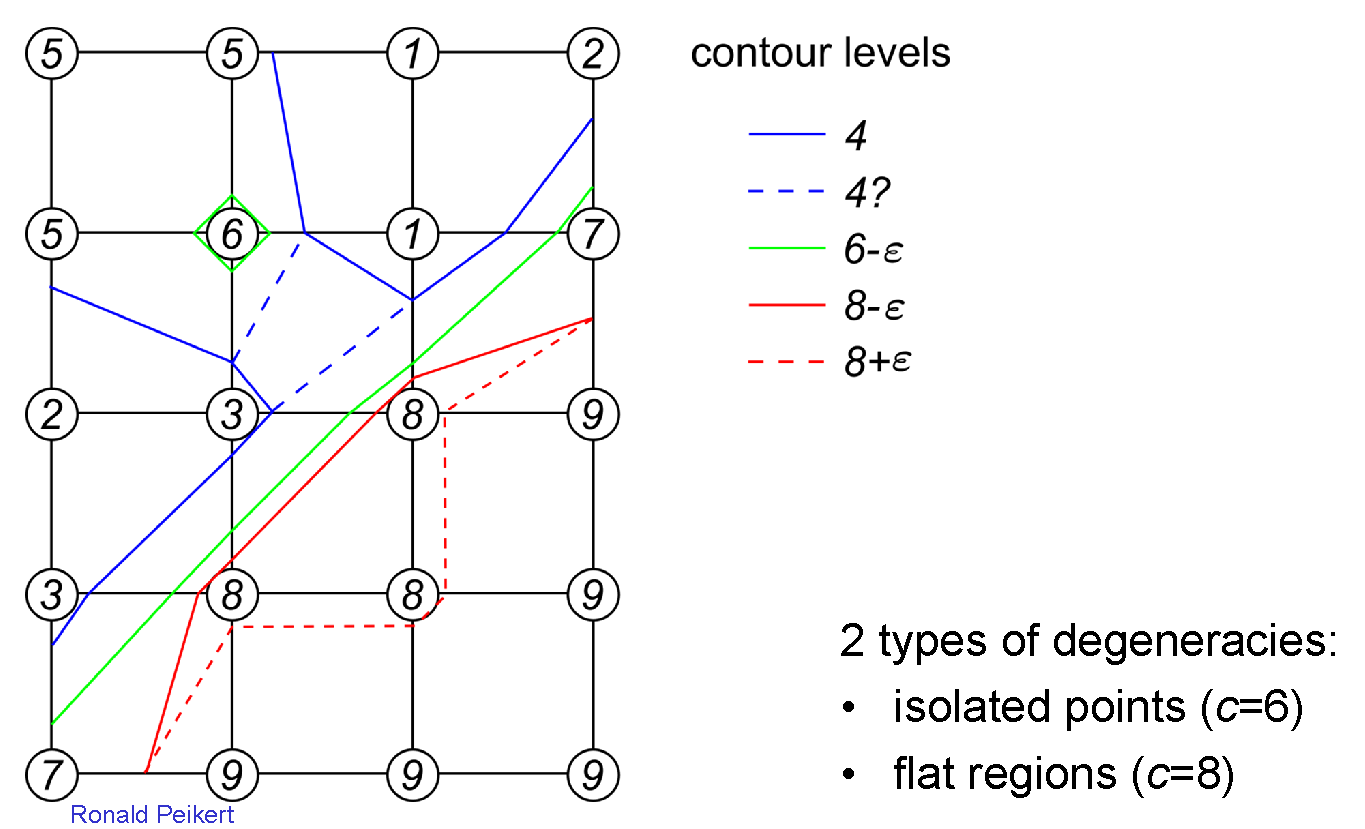
\includegraphics[width=0.75\textwidth]{img/02_contouring_example}
\end{figure}

\paragraph{Topological consistency}
To avoid degeneracies, use \emph{symbolic perturbations}:
\begin{description}
    \item If level $c$ is found as a node value, set the level to $c+\varepsilon$ where $\varepsilon$ is an infinitesimal, i.e., $\varepsilon >0$ and $\varepsilon < x$ $\forall x\in \R$.
\end{description}
Then:
\begin{itemize}
    \item Contours intersect edges at some (possibly infinitesimal) distance from end points.
    \item Flat regions can be visualised by a pair of contours at $c-\varepsilon$ and $c+\varepsilon$.
    \item Contours are \emph{topologically consistent}, meaning:\\
    
        Contours are \emph{closed}, \emph{orientable}, \emph{nonintersecting lines}.    
\end{itemize}

\paragraph{Ambiguities of contours} What is the \emph{correct} contour of $c=4$? 
\begin{figure}[H]
    \centering
    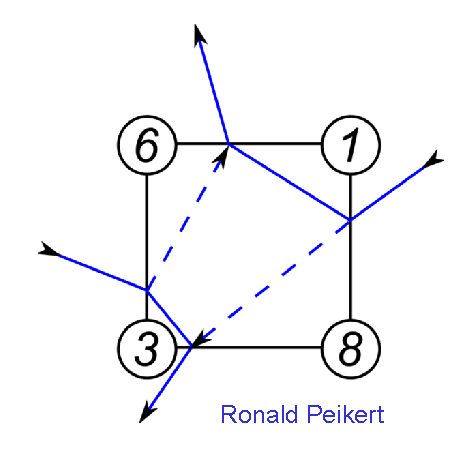
\includegraphics[width=0.3\textwidth]{img/02_contouring_c_4}
\end{figure}
Two possibilities (from which both are orientable):
\begin{itemize}
    \item Connecting the high values \rule{2cm}{0.9pt}
    \item Connecting the low values $- - - - - -$
\end{itemize}

\subsubsection{Contours in a quadrangle cell} 
\begin{description}
\item Local Coordinates $(0,0)\quad (1,0)\quad (0,1)\quad (1,1)$
\item Function Values $\quad s_{00}\quad s_{10}\quad s_{01}\quad s_{11}$
\item Bilinear Interpolant 
    \begin{align*}
     s(x,y) &= (1-x)(1-y)\ s_{00} + x(1-y) \ s_{10}+(1-x)y\ s_{01} + xy\ s_{11}\\
       &= Axy + Bx + Cy + D\\
       \text{with }\quad A &= s_{11}-s_{01}-s_{10}-s_{00}\\
       B &= s_{10}-s_{00}\\
       C &= s_{01}-s_{00}\\
       D &= s_{00}
    \end{align*}
\end{description}

\begin{itemize}
    \item If $A=0$, then the contour equation is $c=Bx+Cy+D$ and the contours are \emph{straight lines}, all parallel.
    \item If $A\neq 0$, then the contour equation is 
        \begin{align*}
            c = A\left( x+{C\over A}\right) (y+{B\over A})+D-{BC\over A}
        \end{align*}
        and the contours are \emph{hyperbola} except for the level
        \begin{align*}
            c = D- {BC\over A}.
        \end{align*}
        
        
        For the special level the contour equation is
            \begin{align*}
                0 = A\left( x+{C\over A}\right) \left( y+{B\over A}\right),
            \end{align*}
        and the contour is a pair of axis-aligned straight lines with
        \begin{align*}
            x &= -{C\over A},\\
            y &= -{B\over A}.
        \end{align*}
\end{itemize}

Decision can be made without computing special level or saddle points by just comparing fractions of edges:
\begin{figure}[H]
    \centering
    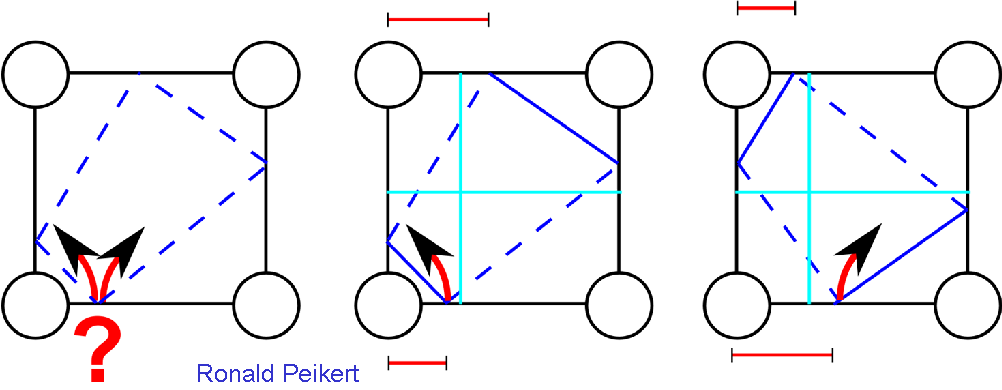
\includegraphics[width=0.75\textwidth]{img/02_contouring_decision}
\end{figure}
By using local coordinates, this works also for curvilinear and unstructured grids.

Not that drawing hyperbola instead of straight lines does not lead to better contours: The piecewise bilinear function is not in $C^1$.

\subsubsection{Basic contouring algorithms}
\begin{description}
    \item[Cell-By-Cell algorithms:] Simple structure, but generate disconnected segments and require post-processing.
    \item[Contour Propagation methods:] Complicated, but generate connected contours.
    \item[Marching Squares algorithm:] Systematic cell-by-cell algorithm. (See below)
\end{description}

\subsubsection{Marching Squares}
Process nodes in ccw (counter-clockwise order), denoted here as $x_0$, $x_1$, $x_2$ and $x_3$. At each node $x_i$ compute the reduced field
\begin{align*}
    \tilde s (x_i) &= s(x_i) - (c-\varepsilon) &\text{(which is forced to be nonzero)}.
\end{align*}
Take it's signe as the $i^{th}$ bit of a $4$-bit integer. Use this as an index for the lookup table containing the connectivity information.
\begin{figure}[H]
    \centering
    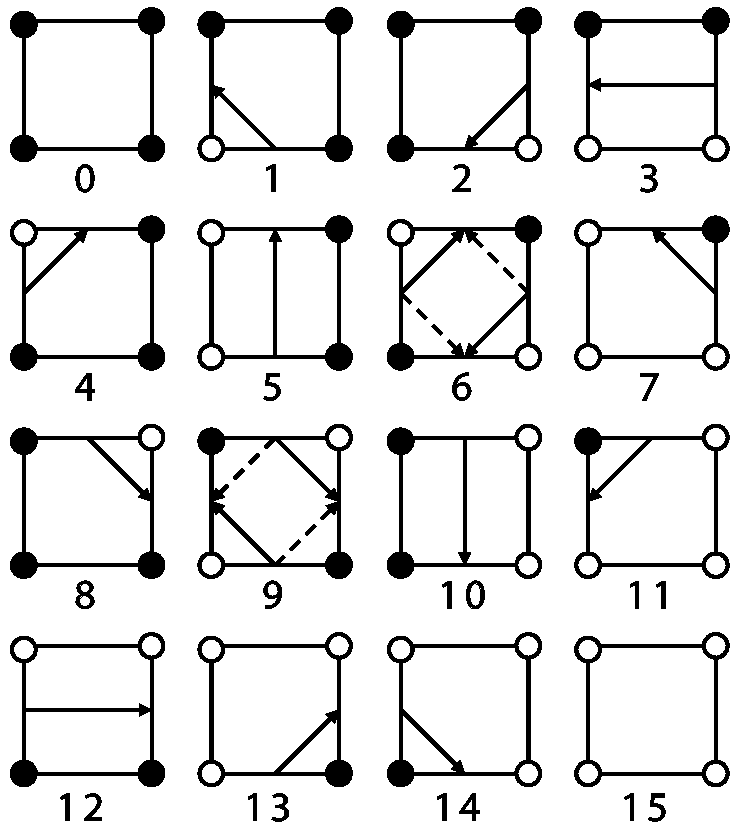
\includegraphics[width=0.5\textwidth]{img/02_marching_squares}
\end{figure}
\begin{align*}
   \bullet\quad \tilde s(x_i) &<0\\
   \circ\quad \tilde s(x_i) &>0
\end{align*}

Alternating signs exist in cases $6$ and $9$. Chose the solid or the dashed line based on topological \emph{consitency}.

\paragraph{Contours in triangle/tetrahedral cells} Linear interpolation of cells implies piece-wise linear contours. Since contours are unambiguous let us introduce a "marching triangles" method. This however introduces periodic artefacts.

\subsection{The Marching Cubes Algorithm}
Contours of $3$D scalar fields are known as \emph{isosurfaces}. Before 1987, isosurfaces were computed as contours on planar \emph{slices}, followed by "contour stitching".

The \emph{marching cubes} algorithm computes contours \emph{directly in 3D}:
\begin{itemize}
    \item Pieces of the isosurfaces are generated on a cell-by-cell basis.
    \item Similar to marching squares, an $8$-bit number is computed from the $8$ signs of $\tilde s(x_i)$ on the corners of a hexahedral cell.
    \item The isosurface piece is looked up in a table with $256$ entries.
\end{itemize}

How to build up the table of $256$ cases?

Lorensen and Cline (1987) exploited $3$ types of symmetries:
\begin{itemize}
    \item Rotational symmetries of the cube
    \item Reflective symmetries of the cube
    \item Sign changes of $\tilde s(x)$.
\end{itemize}

They published a reduced set of $14$ cases:
\begin{itemize}
    \item White circle indicate positive signs of $\tilde s(x)$ ,
    \item The positive side of the isosurface is drawn in red, the negative side in blue.
\end{itemize}

\begin{figure}[H]
    \centering
    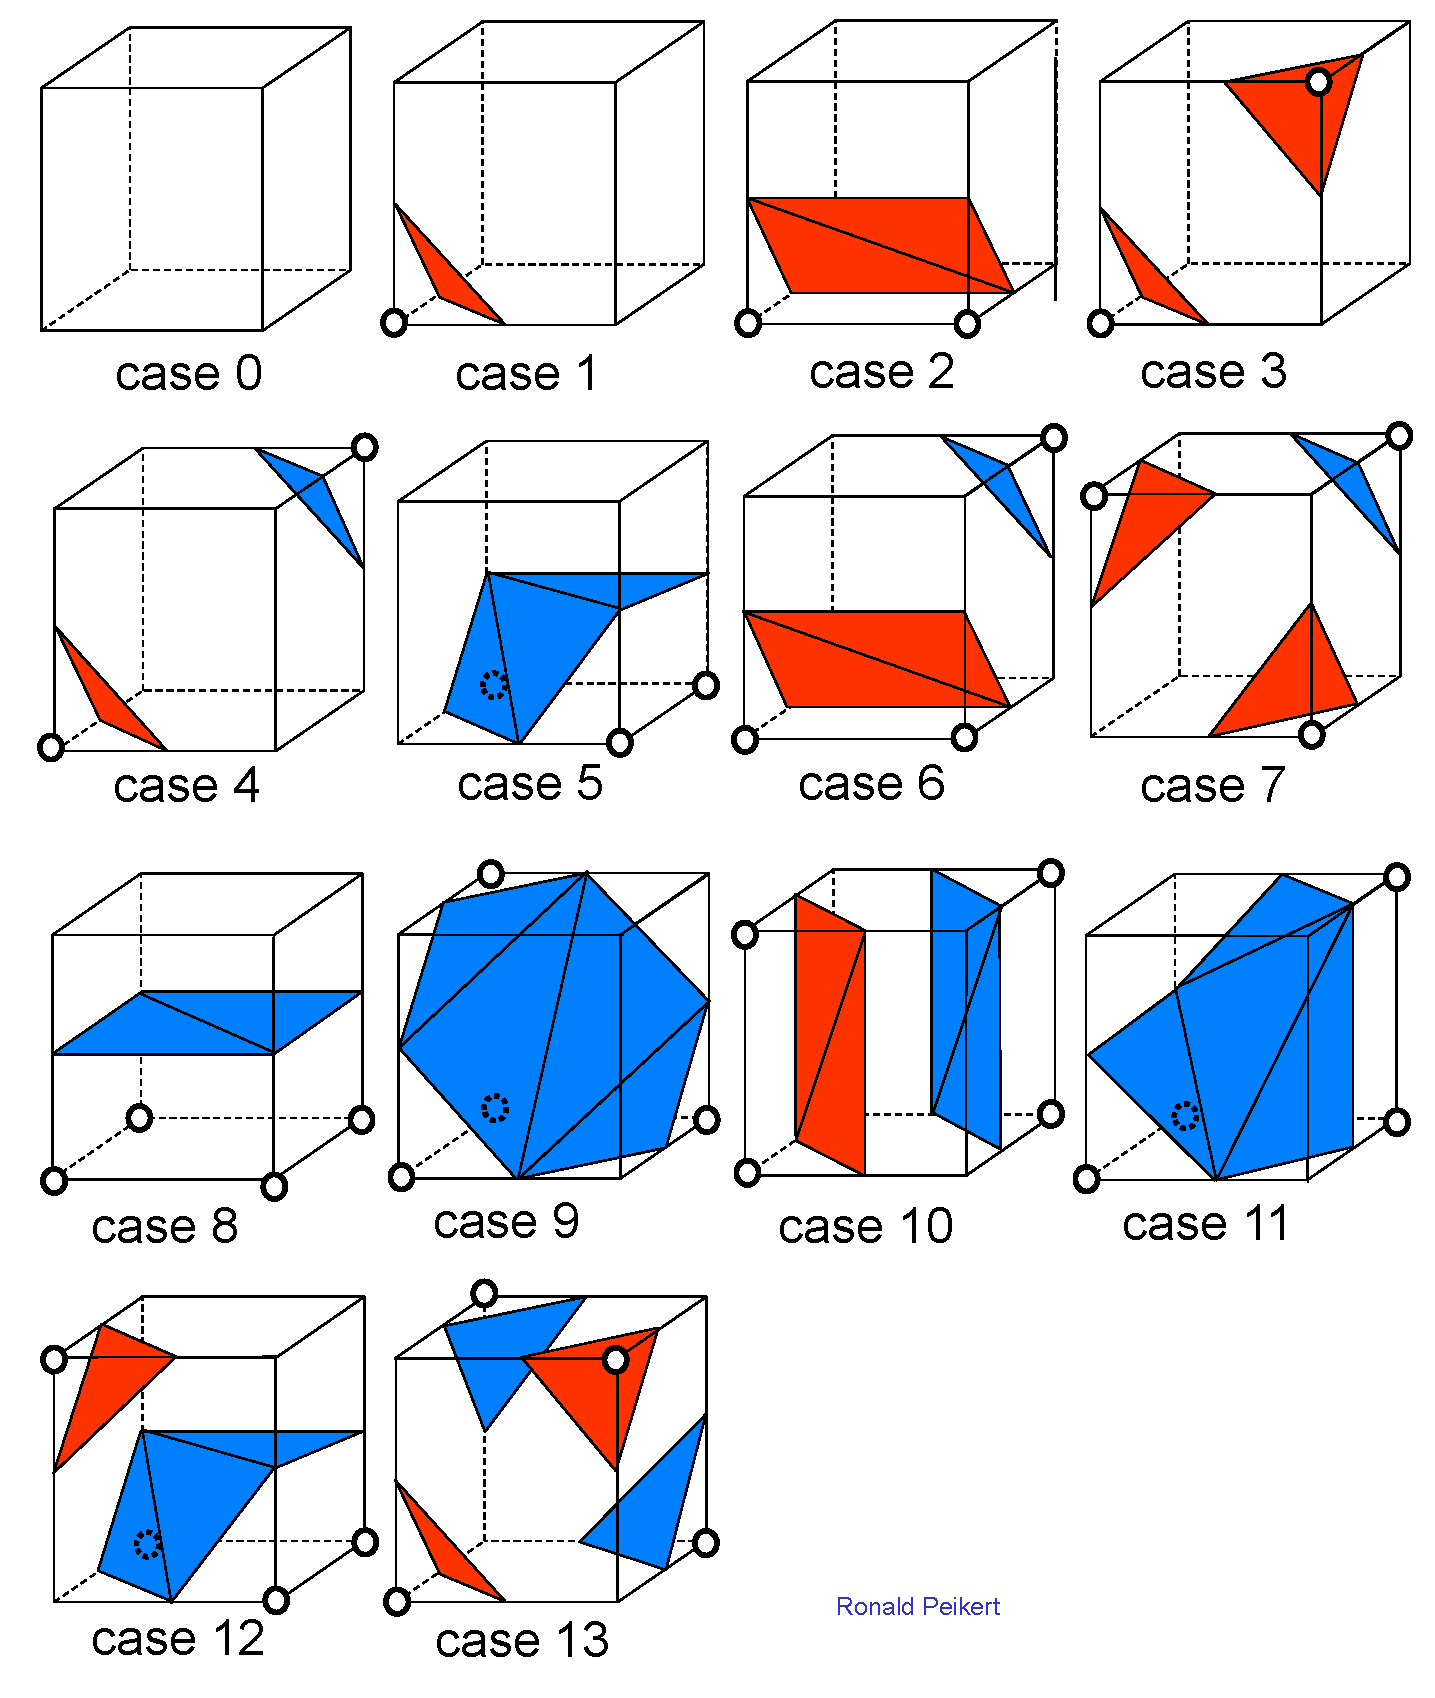
\includegraphics[width=0.75\textwidth]{img/02_marching_cubes}
\end{figure}

Unfortunately not all pieces fit together (same problem as with marching squares) and additional cases need to be introduced. 
\begin{figure}[H]
    \centering
    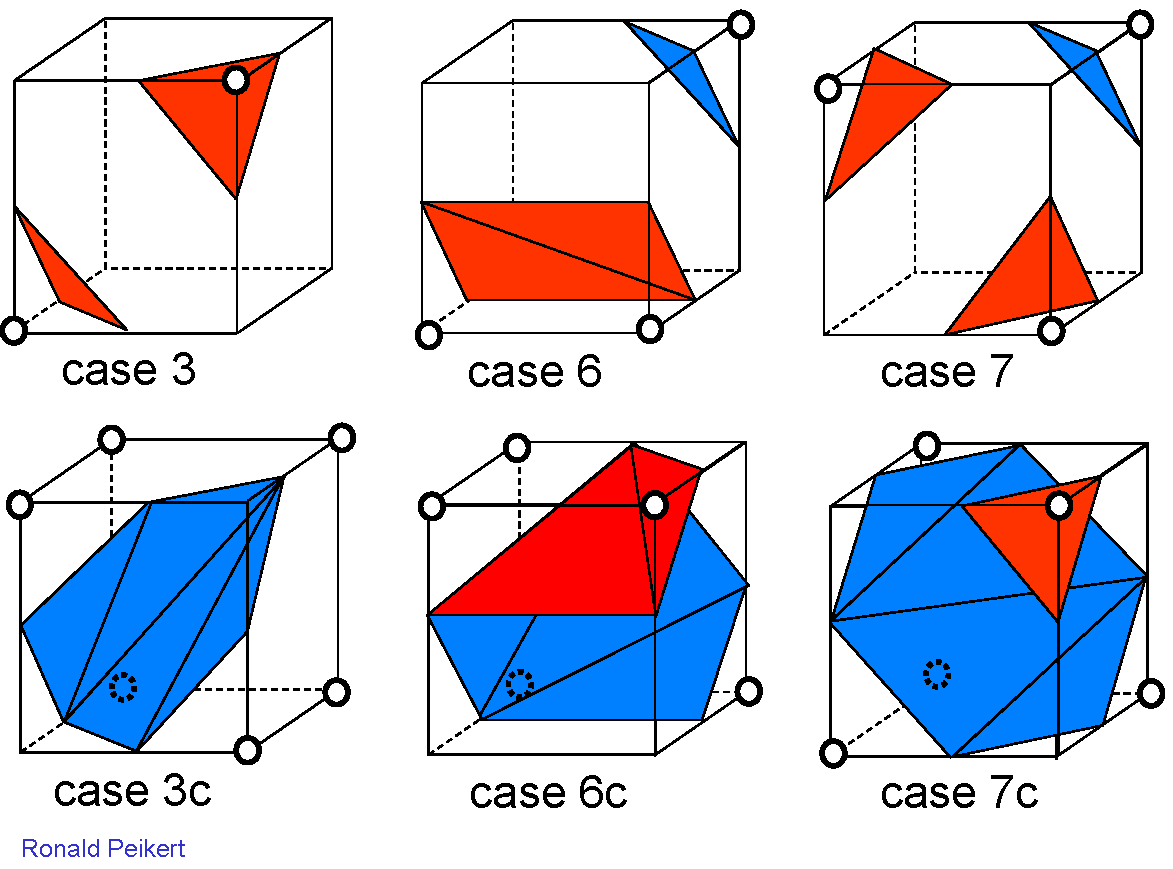
\includegraphics[width=0.75\textwidth]{img/02_marching_cubes_additional_cases}
\end{figure}

The remaining complementary cases are simply obtained by changing the the orientation. Based on these $28$ cases, the full $256$ cases are obtained by rotations of the cube.

\paragraph{Summary} of the algorithm:
\begin{enumerate}
    \item Pre-processing:
        \begin{itemize}
            \item Build a table of the $28$ cases.
            \item Derive a table of the $256$ cases, containing info on
            \begin{itemize}
                \item Intersected cell edges
                \item Triangles based on these points
            \end{itemize}
        \end{itemize}
    \item Loop over cells:
        \begin{itemize}
            \item Find sign of $\tilde s(x)$ for the $8$ corner nodes, giving $8$-bit integer.
            \item Use as index into lookup table.
            \item Find intersection points on edges listed in table, use linear interpolation.
            \item Generated triangles according to table.
        \end{itemize}
    \item Post-processing steps:
        \begin{itemize}
            \item Connect triangles (share vertices)
            \item Compute normal vectors:
                \begin{itemize}
                    \item By averaging triangle normals (problem: thin triangles!).
                    \item By estimating the gradient of the field $s(x)$ (better).
                \end{itemize}
        \end{itemize}
\end{enumerate}

\subsection{The Asymptotic Decider Algorithm}
Motivation for a different isosurface algorithm: Marching cubes can produce "bad" topology.

\emph{Asymptotic decider} algorithm (Nielson and Hamann 1991):
\begin{itemize}
    \item Generate topologically \emph{correct} contours (as oriented straight line segments) on the cell surfaces.
    \item Connect these around the cell, resulting in one or more polygons.
    \item Triangulate the polygons.
\end{itemize}
In general, the AD algorithm generates better isosurfaces. However,
\begin{itemize}
    \item It cannot be easily implemented with a table like Marching Cubes (too many cases).
    \item It generates polygons with up to $12$ sides (Marching Cubes: up to 7).
    \item The topology is correct with respect to the trilinear interpolant, but the geometry can deviate.
    \item Some polygons cannot be "cleanly" triangulated.
\end{itemize}

\subsection{The Dividing Cubes Algorithm}
An early \emph{point-based} algorithm (Crawford et al. '87): For each cell
\begin{itemize}
    \item Check whether it is intersected by the isosurface:
        \begin{align*}
            \min_{i\in \text{cell}} s_i < c < \max_{i\in \text{cell}} s_i
        \end{align*}
    \item Subdivide the intersected cell into $m\times m\times m$ subcells using trilinear interpolation.
    \item Draw the centers of all intersected subcells.
    \item To light the points estimate the gradient and use it as the normal vector.
\end{itemize}

\subsection{Optimised Isosurface Algorithms}
Approaches to speeding up isosurface computation:
\begin{description}
\item[View Dependent] algorithms:
    \begin{itemize}
        \item Occluded triangles are not computed
        \item GPU-based isosurface computation and redenring
    \end{itemize}
\item[Data Processing] for fast computation of \emph{multiple} isosurfaces (multiple levels), for example for interactive exploration of the data.
    \begin{itemize}
        \item Many methods: Octree, Extrema Graph, Span Space.
        \item Common Goal: Avoid computation in non-intersected cells.
    \end{itemize}
\end{description}

\subsubsection{The Span-Space Algorithm}
Method by Livnat (1996).
\begin{enumerate}
\item Pre-Processing. For each element
    \begin{itemize}
        \item Compute $\min$ and $\max$ ,
        \item Treat $(\min,\max)$ as a point in the \emph{span space} (Euclidean plane).
        \item Store points in boxes, non-empty boxes are stored in a linked list.
    \end{itemize}
\item Computation of the isosurface level $c$:

    Find the intersected cells in the \emph{quadrant} $\min < c$, $\max > c$.
    \begin{figure}[H]
    \centering
        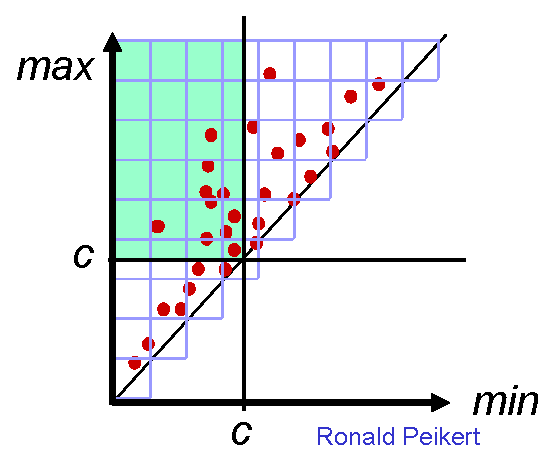
\includegraphics[width=0.5\textwidth]{img/02_span_space_algorithm}    
        \caption{Node distribution in span space.}
    \end{figure}

\end{enumerate}

This algorithm yields a performance gain for datasets with a small local variation, i.e. points in the span space are distributed on the diagonal.

\subsection{Selecting Contour Levels}
Several types of isosurface statistics can help with level selection. 
\begin{figure}[H]
\centering
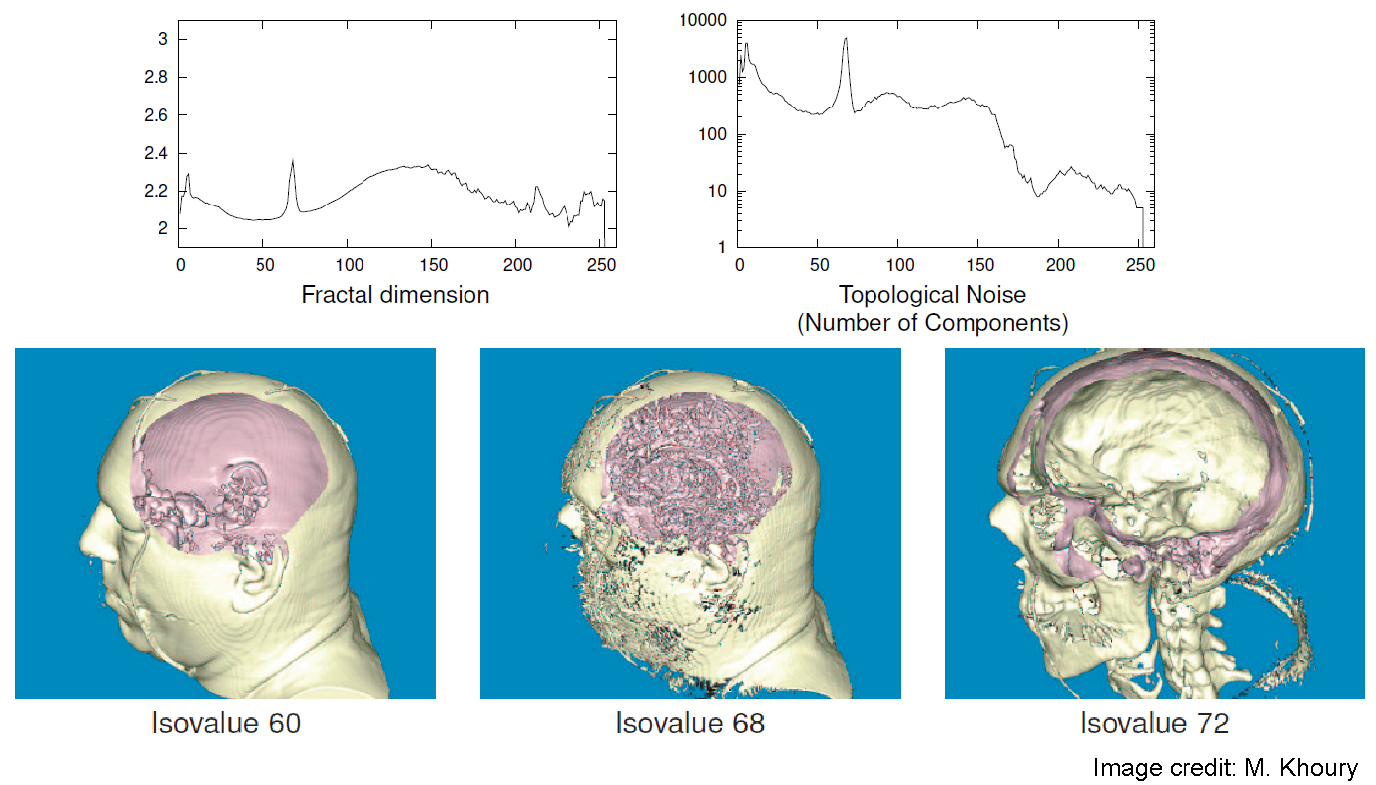
\includegraphics[width=0.9\textwidth]{img/02_contouring_statistics}
\end{figure}

\subsection{Limitations of Isosurfaces}
Isosurfaces represent only a single level within the data range. In practical data, there is often not a single "interesting" level.

Transparent rendering of multiple isosurfaces is possible, but
\begin{itemize}
    \item Limited to a small number of surfaces by visibility
    \item Alpha-blending require depth sorting.
\end{itemize}

Alternatives:
\begin{itemize}
    \item \emph{Feature Extraction methods}, e.g. detecting "blobs" (maximal ellipse-like contours)
    \item \emph{Volume rendering} can show ranges of "interesting levels of the field and/or its gradient.
\end{itemize}








\newpage
\section{Raycasting}

\subsection{Direct Volume Rendering}

Volume rendering (sometimes called \emph{direct volume rendering}) stands for methods that generate images directly from $3$D scalar data. "Directly" means: \emph{no intermediate geometry} (such as an isosurface) is 
generated.

Volume rendering techniques
\begin{itemize}
    \item Depend strongly on the grid type.
    \item Exist for structured and unstructured grids.
    \item Are predominantly applied to uniform grids with $2$D or $3$D image data with \emph{cell-centered} data.
    Cell-centered data 
    \begin{itemize}
        \item are attributed to cells (pixels, voxels) rather than nodes,
        \item can also occur in (finite volume) CFD datasets,
        \item are converted to node data:
            \begin{itemize}
                \item By taking the \emph{dual grid} (easy for uniform grids: $n$ cells $\rightarrow$ $n-1$ cells!),
                \item or by interpolating. 
            \end{itemize}
    \end{itemize}
\end{itemize}


\subsection{Raycasting}
\emph{Raycasting} is historically the first volume rendering technique. It is very similar to \emph{raytracing}:
\begin{itemize}
    \item \emph{image-space} method: The main loop iterates over the pixels of the output image,
    \item a \emph{view ray} per pixel (or per subpixel) is traced backward,
    \item and samples are taken along the ray and \emph{composited} to a single color.
\end{itemize}
The differences are
\begin{itemize}
    \item No secondary (reflected, shadow) rays,
    \item the transmitted ray is not refracted,
    \item more elaborate compositing functions,
    \item and samples are taken at intervals (not at object intersections).
\end{itemize}

\subsubsection{Compositing}
Two simple compositing functions can be used for previewing:
\begin{description}
    \item[Maximum intensity projection] (MIP):
        \begin{itemize}
            \item Maximum of sampled values
            \item Result resembles X-ray image.
        \end{itemize}
    \item[Local maximum Intensity projection] (LMIP):
        \begin{itemize}
            \item Choose first local maximum which is above a prescribed threshold.
            \item Process approximates occlusion.
            \item It is faster and better than MIP.
        \end{itemize}
        \begin{figure}[H]
            \centering
            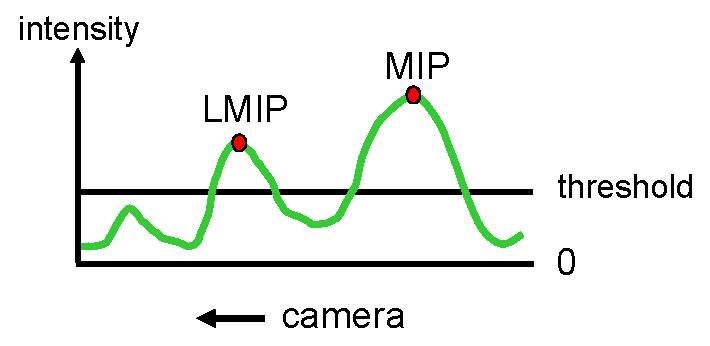
\includegraphics[width=0.6\textwidth]{img/03_lmip}
        \end{figure}
\end{description}

\subsubsection{$\alpha$-compositing}
Assume that each sample on a view ray has a \emph{color} and \emph{opacity}.
\begin{align*}
    (C_0,\alpha_0), \ldots, (C_N,\alpha_N)\qquad\qquad C_i\in [0,1]^3,\ \ \alpha_i\in [0,1]
\end{align*}
where the $0^{th}$ sample is next to the camera and the $N^{th}$ one is a (fully opaque) background sample:
\begin{align*}
    C_N &= (r,g,b)_\text{background}\\
    \alpha_N &= 1.
\end{align*}
$\alpha$-compositing can be defined recursively:

Let $C_f^b$ denot the \emph{composite color} of samples $f$, $f+1$, $\ldots$, $b$. The recursion formula for \emph{back-to-front} compositing yields:
\begin{align*}
    C_b^b &= \alpha_b C_b\\
    C_f^b &= \alpha_f C_f + (1-\alpha_f)C_{f+1}^b.
\end{align*}
With \emph{transparency} set to $T_i = 1-\alpha_i$ we get a \emph{closed formula} for $\alpha$-compositing:
\begin{align*}
    C_f^b = \sum_{i=f}^b \alpha_i C_i \prod_{j=f}^{j-1} T_j
\end{align*}
The \emph{front-to-back} compositing can be derived from the closed formula: Let $T_f^b$ denote the \emph{composite transparency} of samples $f$, $f+1$, $\ldots$, $b$:
\begin{align*}
    T_f^b = \prod_{j=f}^b T_j.
\end{align*}
Then the \emph{simultaneous recursion} for front-to-back composition is:
\begin{align*}
    C_f^f &= \alpha_f C_f\\
    T_f^f &= 1-\alpha_f\\
    C_f^{b+1} &= C_f^b + \alpha_{b+1} C_{b+1} T_f^b\\
    T_f^{b+1} &= (1-\alpha_{b+1})T_f^b.
\end{align*}

\paragraph{The emission-absorption model} How realistic is $\alpha$ compositing? The \emph{emission-absorption} model (Sabella 1988) yields a basic \emph{volume rendering equation}"
\begin{align*}
    L(x) = \int_x^{x_b} \varepsilon (x') \exp\left( -\int_x^{x'} \tau (x'') dx''\right) dx'
\end{align*}
The equation describes the \emph{radiance} arriving along a ray at the position $x$ on this ray. The \emph{emission} function $\varepsilon(x)$ describes the photons "emitted" by the volume along the ray. The \emph{absorbtion} function $\tau(x)$ is the probability that that photon traveling over a unit distance is lost by absorption.


The emission-absorption model is based on the Boltzmann transport equation in statistical physics, but completely \emph{ignores scattering}. In more general models $\tau(x)$ is an \emph{extinction function} having both an absorption term and a scattering term.

Instead, in the emission-absorption model:
\begin{itemize}
\item \emph{Incident scattering} is modelled by the emission function
\item \emph{Loss by scattering} can be thought to be part of the absorption.
\end{itemize}


The discrete version of the emission absorption model:
\begin{align*}
    L(x) = \sum_{i=0}^n \varepsilon_i \Delta x \exp\left( -\sum_{j=0}^{i-1} \tau_j \Delta x \right) 
    = \sum_{i=0}^n \varepsilon_i \Delta x\prod_{j=0}^{i-1} e^{- \tau_j \Delta x},
\end{align*}
matches the $\alpha$-compositing formula
\begin{align*}
    C_f^b = \sum_{i=f}^b \alpha_i C_i \prod_{j=f}^{j-1} (1-\alpha_i)
\end{align*}
and gives interpretations of "opacity" and "color":
\begin{align*}
    \alpha_i &= 1-e^{\tau_j\Delta x} \approx \tau_j \Delta x &\text{if }\Delta x << 1\\
    \alpha_i C_i &= \varepsilon_i \Delta x.
\end{align*}

The product $\tilde C = \alpha_i C_i$ is called a \emph{premultiplied} or \emph{associated} colour.

\subsection{Transfer Functions}
\emph{Transfer functions} map raw voxel data to opacities and colours as needed for the $\alpha$-compositing. Inputs of the TF (one or more):
\begin{itemize}
    \item Voxel value $s(x)$
    \item Gradient magnitude $\norm{\nabla s(x)}$
    \item Higher derivatives of $s(x)$.
\end{itemize}

\begin{description}
\item \emph{Opacity transfer function} $\alpha(s(x), \norm{\nabla s(x)}, \ldots)$
\item \emph{Color transfer function} $C(s(x), \norm{\nabla s(x)}, \ldots)$
\end{description}

In general TF don't depend on \emph{spatial location}, exception for \emph{focus and context} techniques.

By choosing different opacity transfer functions different types of applications can be achieved.
\begin{figure}[H]
\centering
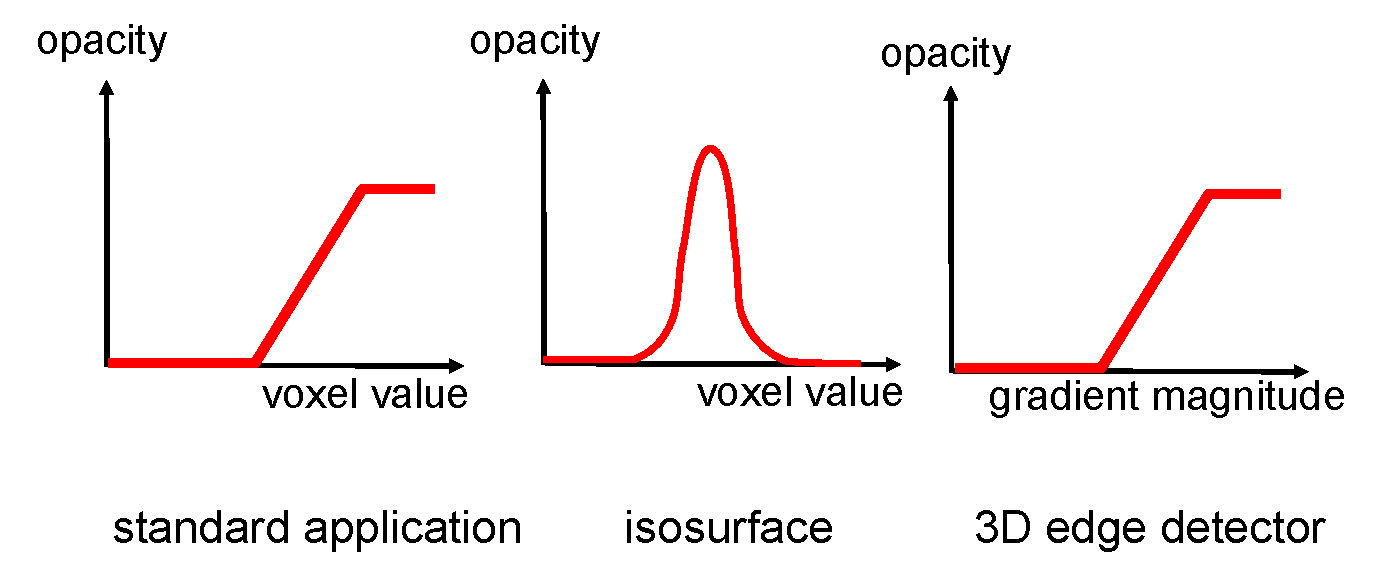
\includegraphics[width=0.8\textwidth]{img/03_tf_types}
\end{figure}

Example of a \emph{bivariate} (=2D) transfer function:
\begin{figure}[H]
    \centering
    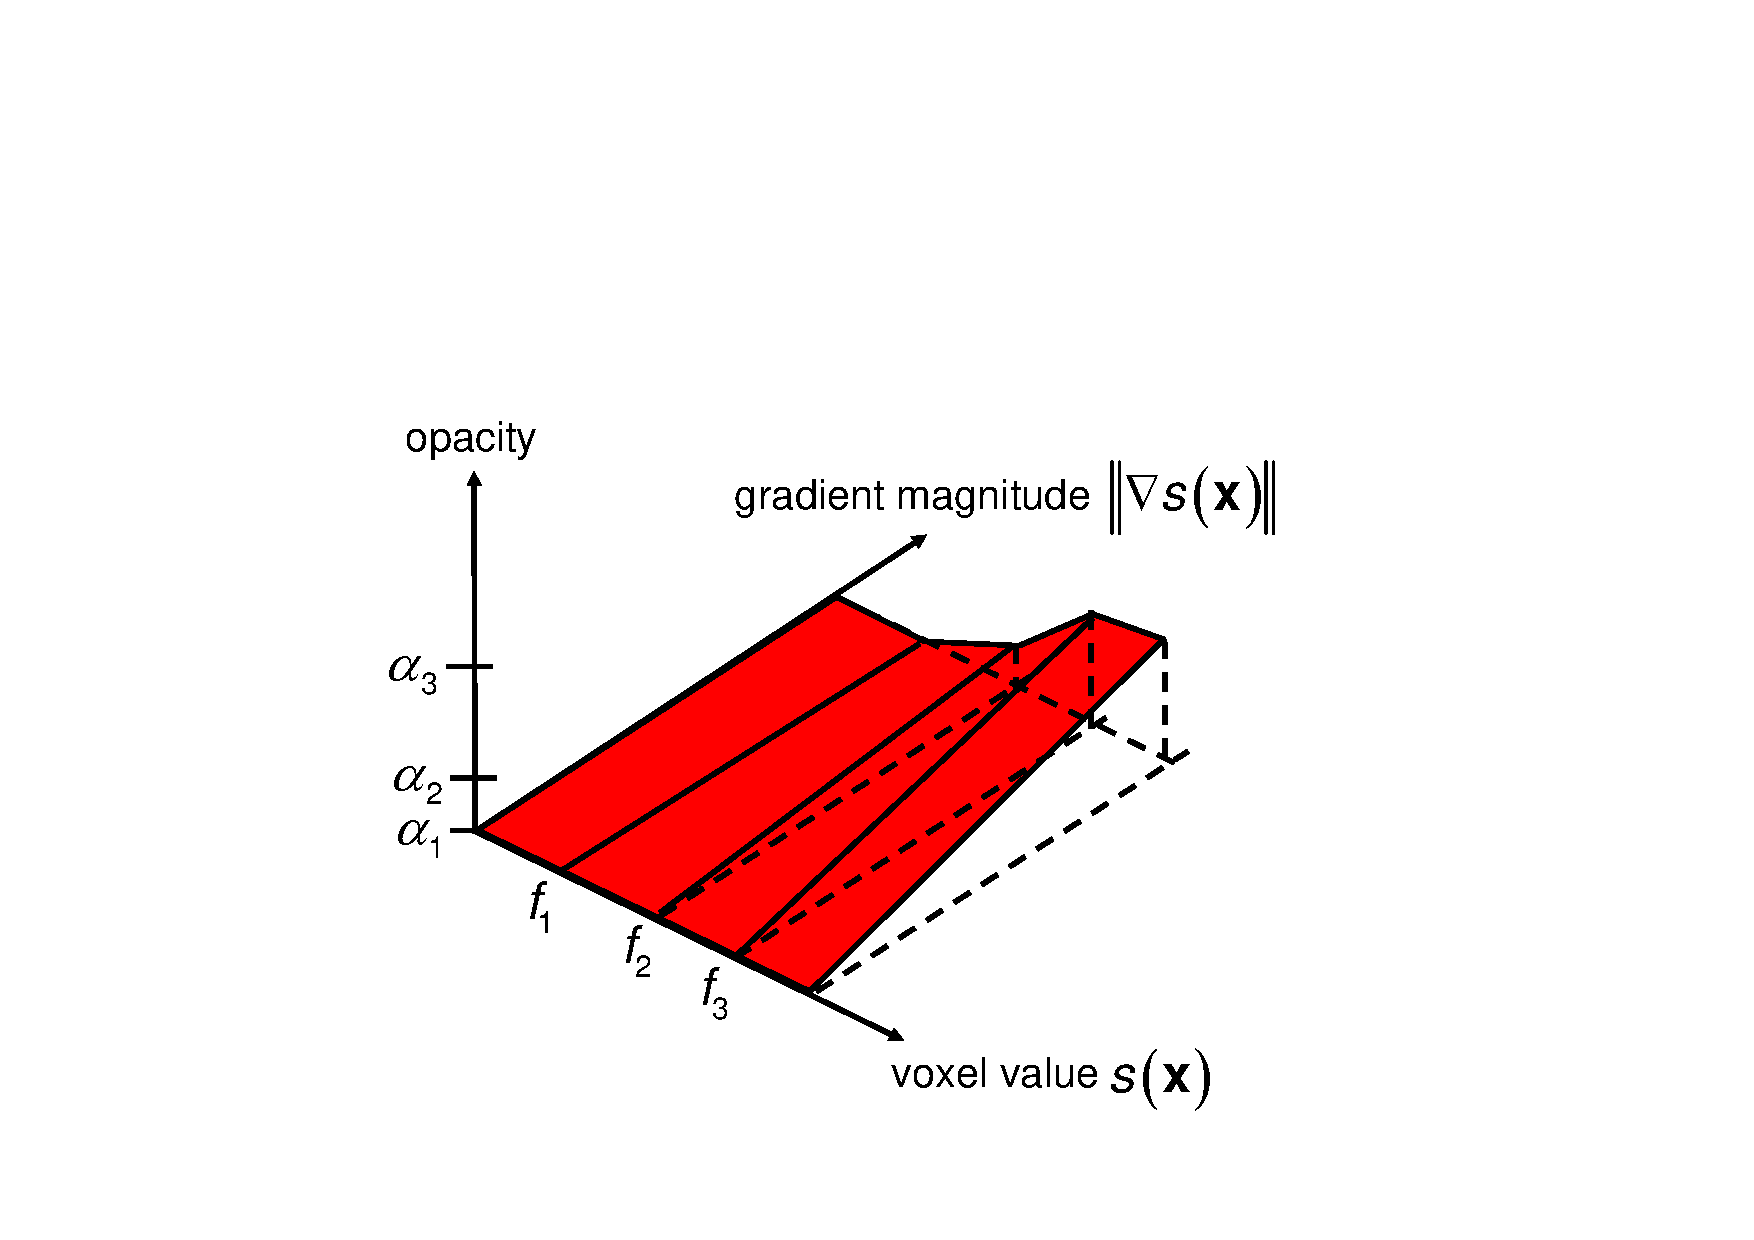
\includegraphics[width=0.6\textwidth,page=1]{img/03_tf_bivariate}
\end{figure}
Example of a bivariate transfer function for an isosurface of constant thickness.
\begin{figure}[H]
    \centering
    \includegraphics[width=0.6\textwidth,page=2]{img/03_tf_bivariate}
\end{figure}

The color transfer function allows to make a simple \emph{classification}.
\begin{figure}[H]
    \centering
    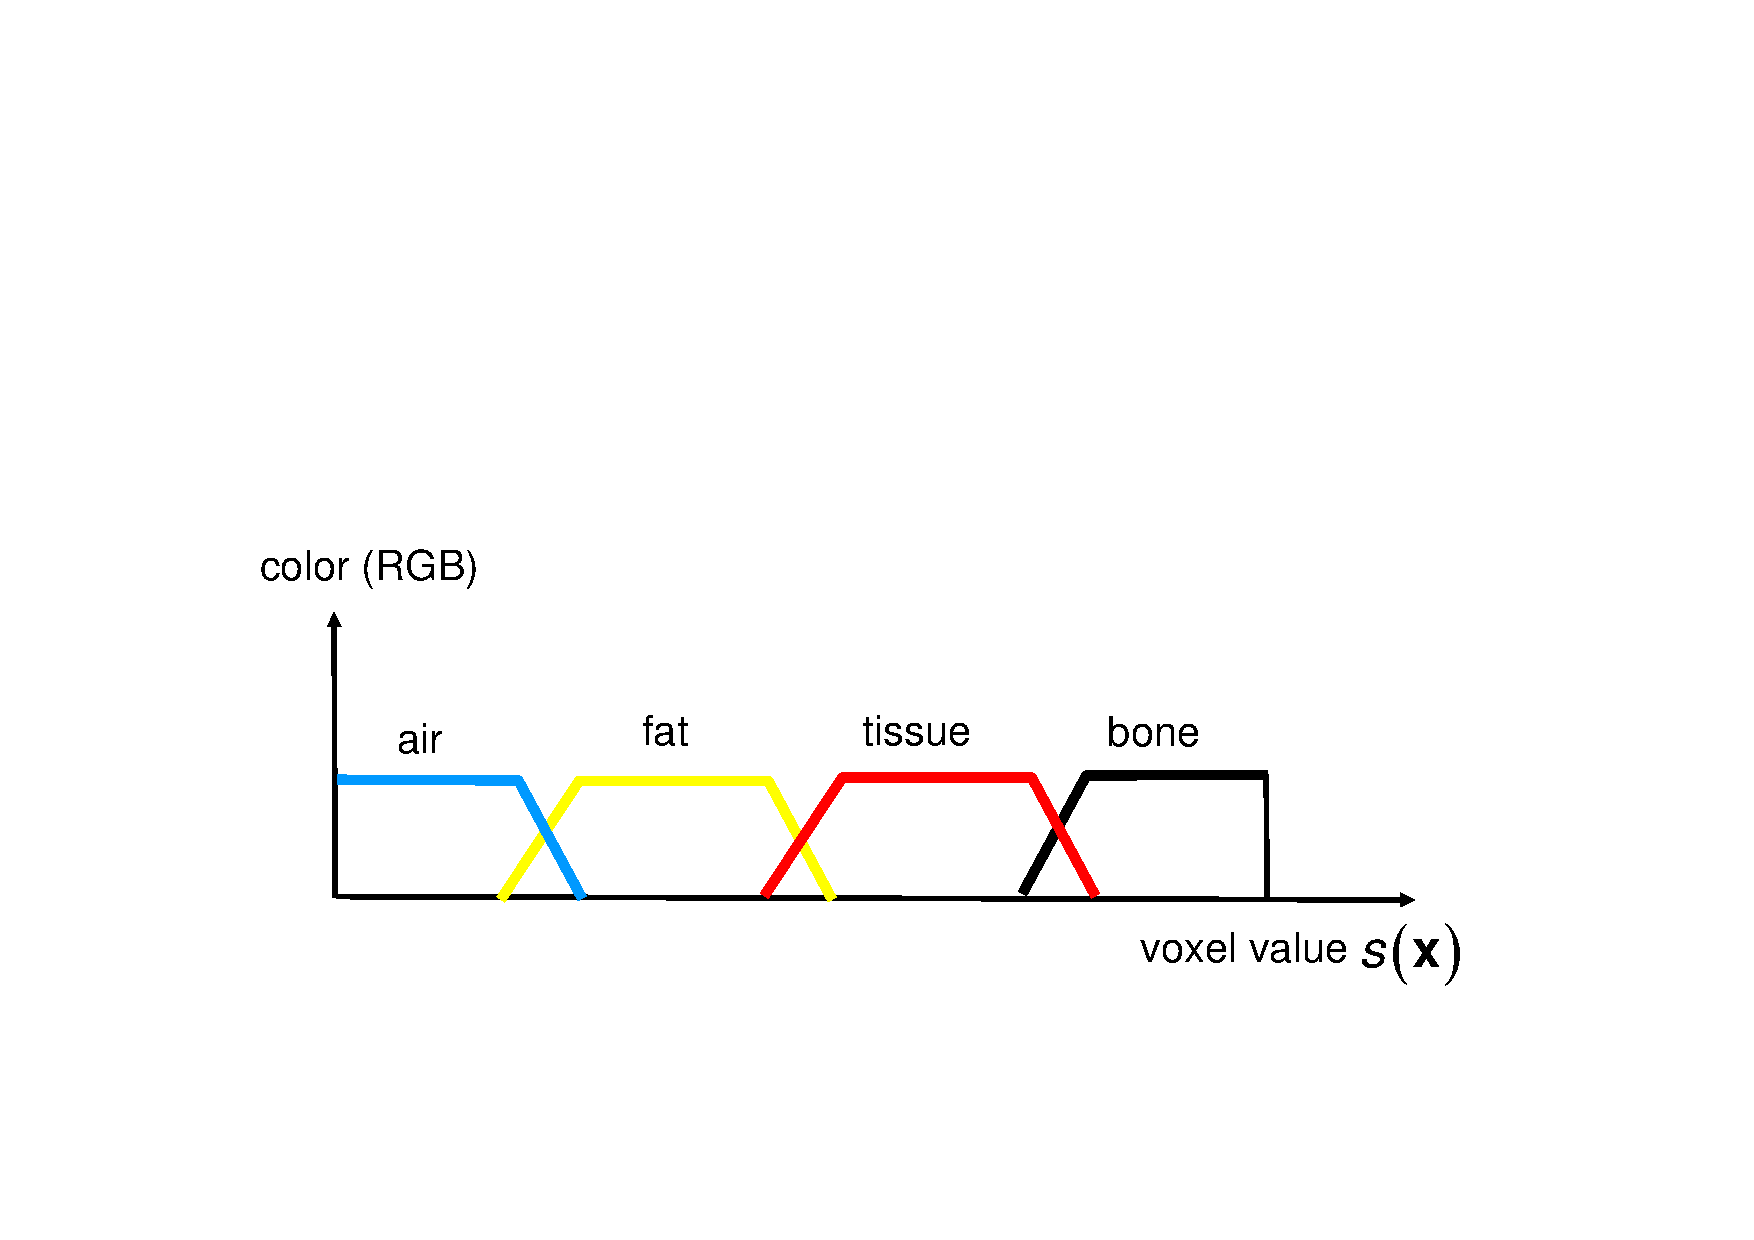
\includegraphics[width=0.8\textwidth,page=1]{img/03_tf_color}
\end{figure}

\paragraph{Pre-classification} In pre-classification, the voxels can also be lit:
\begin{itemize}
    \item The gradient is perpendicular to the local isosurface. It can be used as a normal vector for \emph{Phong lighting} (without rendering the isosurface itself).
    \item \emph{Reflection coefficients} can be assigned by a separate transfer function ("materials" instead of only colors).
    \item \emph{Diffuse lighting} can be applied to the entire volume dataset as a pre-processing since it's independent of the viewing direction.
\end{itemize}

\subsubsection{Pre- vs. Post-classification}
For quality reasons, current volume rendering implementations often use \emph{post-classficiation}.

\begin{description}
\item[Pre-Classification] $\ $
    \begin{enumerate}
        \item Transfer functions are applied to voxels.
        \item Results are interpolated to sample locations.
    \end{enumerate}
\item[Post-Classification] $\ $
    \begin{enumerate}
        \item Raw data are interpolated to sample locations.
        \item Transfer functions are applied to sampled data.
    \end{enumerate}
\end{description}

\subsection{Preintegration}
Idea (Engel 2001): Simulate \emph{infinitely many} interpolated samples between two successive samples $s_i= s(x_i)$ and $s_{i+1} = s(x_{i+1})$. Assuming that 
\begin{itemize}
    \item Field $s(x)$ varies \emph{linearly} between samples
    \item and that the transfer functions don't depend on derivatives.
\end{itemize}

The discrete formula for opacity at a sample was
\begin{align*}
    \alpha_i = 1-e^{-\tau_i \Delta x}.
\end{align*}
The continuous version for a sample interval $[x_i, x_{i+1}]$ is 
\begin{align*}
    \alpha_i = 1-e^{-\int_{x_i}^{x_{i+1}} \tau(s(x)) dx}.
\end{align*}
Assuming now $s(x)$ to be linear between samples, we get:
\begin{align*}
    \alpha_i &= 1-\exp\left( {-{d\over s_{i+1}-s_i} \int_{s_i}^{s_{i+1}}\tau(s) ds}\right) &\text{with } d= \norm{x_{i+1}-x_i}, 
\end{align*}
which is called a \emph{preintegrated opacity transfer function}.


The integral
\begin{align*}
\int_{s_i}^{s_{i+1}} \tau(s) ds = \int_0^{s_{i+1}} \tau(s) ds - \int_0^{s_i} \tau(s)ds
\end{align*}
can be evaluated by two lookups in a precomputed table of 
\begin{align*}
\int_0^{s} \tau(s')ds'.
\end{align*}

The composite colour of the same interval
\begin{align*}
  C_i = \int_{x_i}^{x_{i+1}} \varepsilon (s(x))\exp\left(-\int_{x_i}^x \tau(s(x'))dx'\right) dx,
\end{align*}
simplifies for linear $s(x)$ to:
\begin{align*}
  C_i = {d\over {s_{i+1}-s_i}} \int_{s_i}^{s_{i+1}} \varepsilon (s)\exp\left(-{d\over {s_{i+1}-s_i}} \int_{s_i}^x \tau(s')ds'\right) ds,
\end{align*}
which can be precomputed for all combinations of $s_i$, $s_{i+1}$ and $d$.

\subsubsection{Extinction-based volume rendering}
Instead of an opacity Transfer function, use an extinction TF [Schlegel 2011]. Advantage: Extinction is \emph{additive}.
\begin{itemize}
    \item Riemann sums for numerical integration give better accuracy.
    \item Additivity can be used for efficient lighting.
\end{itemize}

\paragraph{Screen-Space ambient occlusion} Approximate the fraction of ambient light that is occluded. Method: Compute the total extinction per shell (boxes approximating spheres) b using a \emph{summed area table}.




\newpage
\section{Object Space Volume Rendering}
In object space rendering methods the main loop is not over the pixels but over the objects in $3$-space. In case of direct volume rendering "objects" can mean:
\begin{itemize}
    \item Layers of voxels: Use \emph{Image compositing} methods:
        \begin{itemize}
            \item 2D texture based
            \item 3D texture based
        \end{itemize}
    \item Voxels: Use \emph{splatting} methods.
    \item Cells: Use \emph{cell projection} methods.
\end{itemize}

\subsection{Texture-based volume rendering}
\subsubsection{Volume rendering with 2D texturemapping}
\begin{itemize}
    \item Use planes parallel to the \emph{base plane}. The base plane is the front face of the volume which is "most orthogonal" to the view ray.
    \item Draw the texture rectangles using a bilinear interpolation filter.
    \item Render back-to-front using $\alpha$-blending for the $\alpha$-composition.
\end{itemize}
\begin{figure}[H]
    \centering
    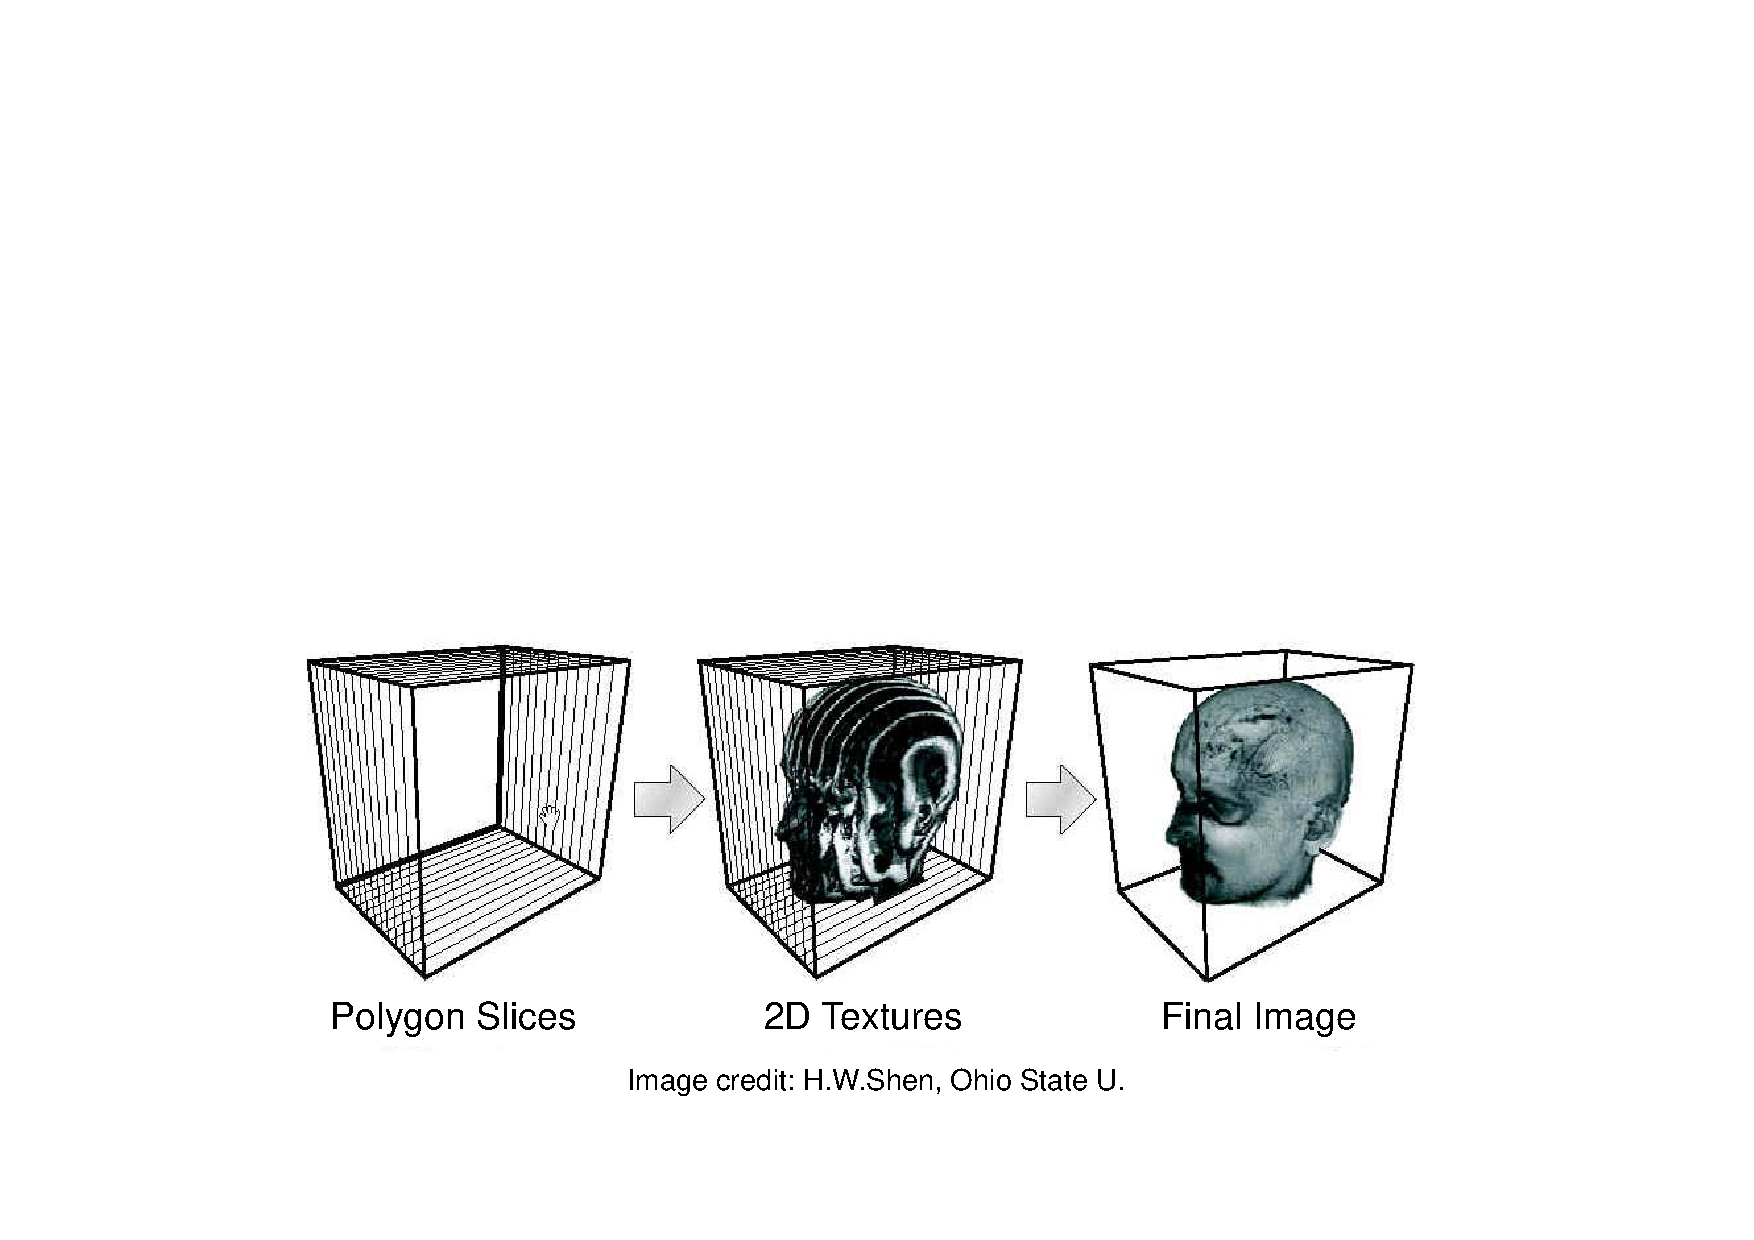
\includegraphics[width=0.8\textwidth]{img/04_texture_based_volume_rendering}
\end{figure}

\subsubsection{Volume rendering with 3D texture mapping}
Cabral 1994.
\begin{itemize}
    \item Use the voxel data as the 3D texture.
    \item Render an arbitrary number of slices (eg. 100 or 1000) parallel to the image plane (3- to 6- sided polygons).
    \item Back-to-front compositing as in the 2D texture method.
\end{itemize}
This method is limited by the size of the texture memory. 
\begin{figure}[H]
    \centering
    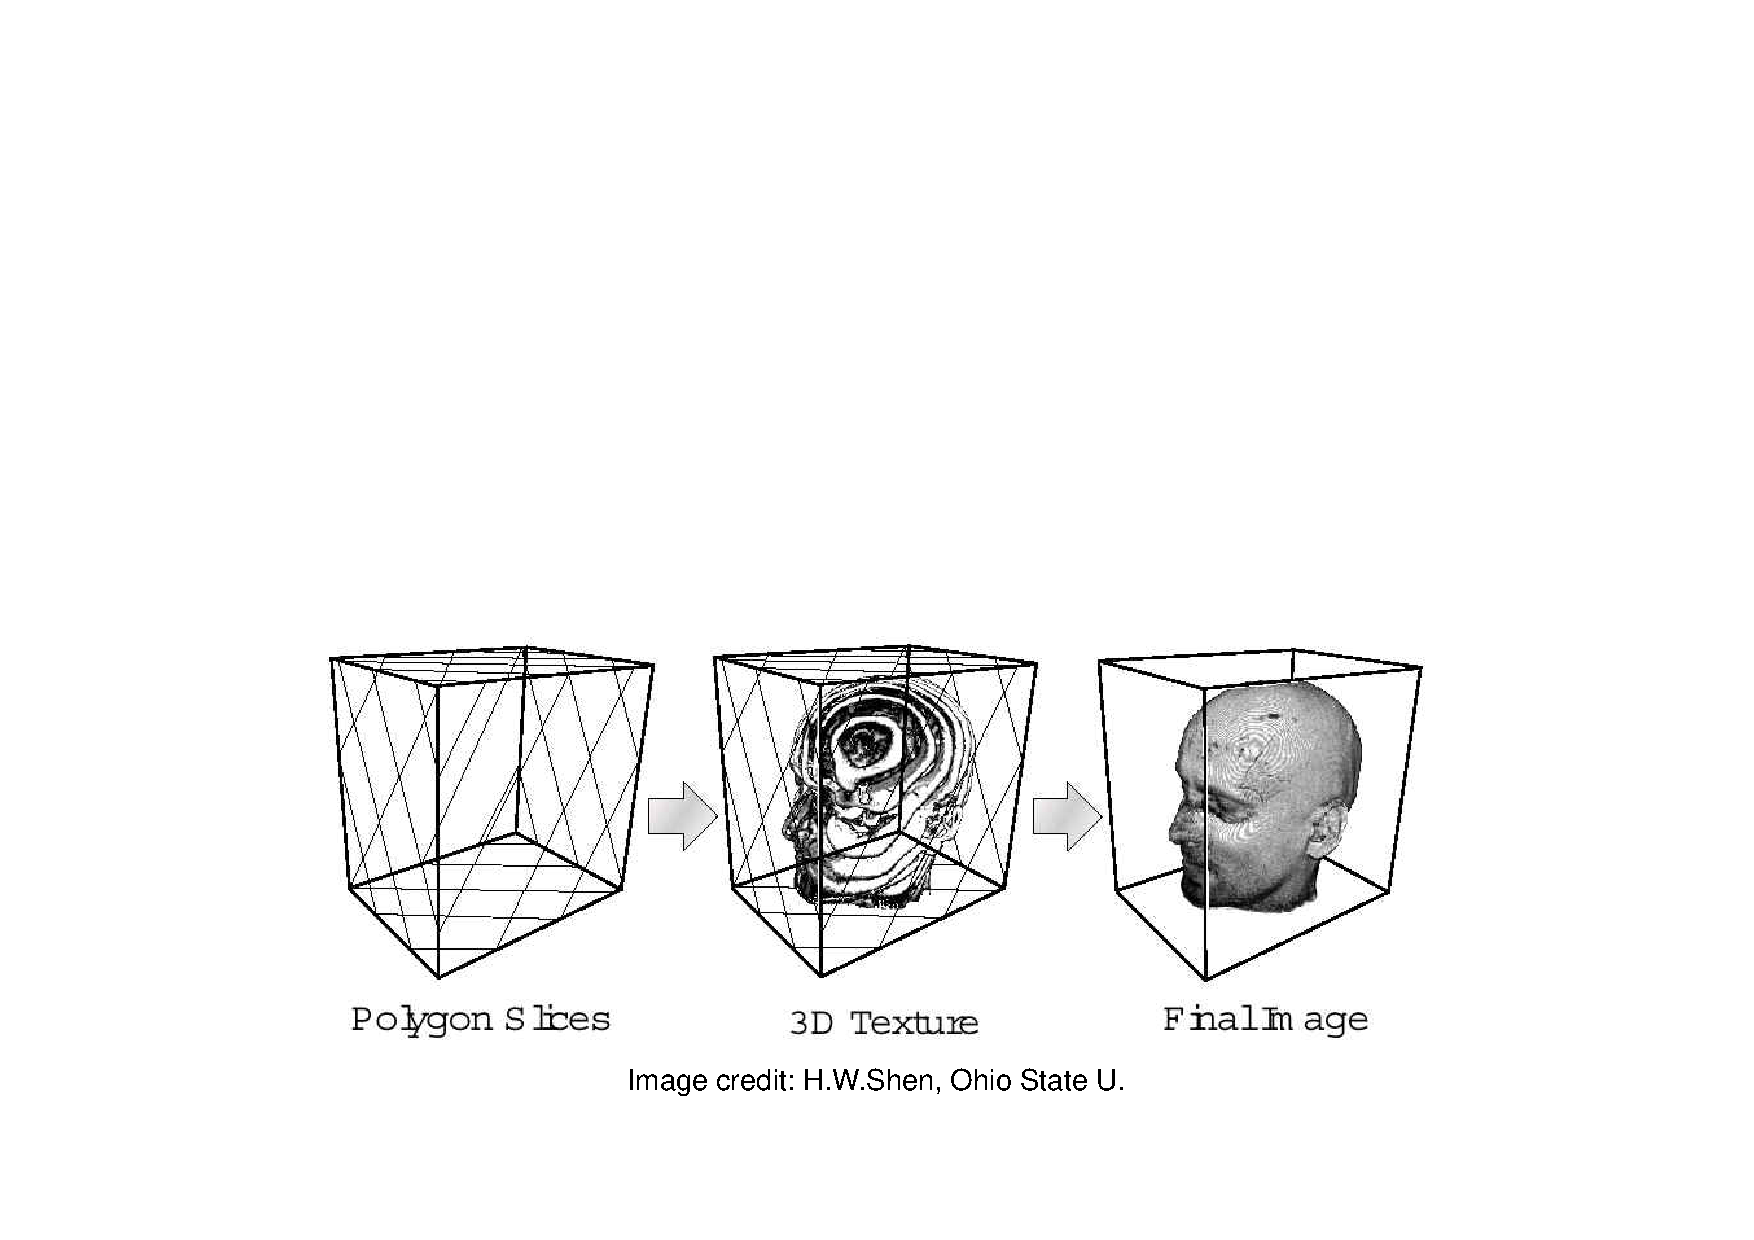
\includegraphics[width=0.8\textwidth]{img/04_3dtexture_based_volume_rendering}
\end{figure}

\subsection{Shear-Warp Factorisation}
In general the image plane is not parallel to a volume face. The \emph{shear-warp} method allows to render an intermediate image in the base plane:
\begin{enumerate}
    \item Transform the \emph{sheared object space} by translating (and possibly scaling) the voxel layers.
    \item \emph{Render} the intermediate image in the base plane.
    \item \emph{Warp} the intermediate image.
\end{enumerate}
\begin{figure}[H]
    \centering
    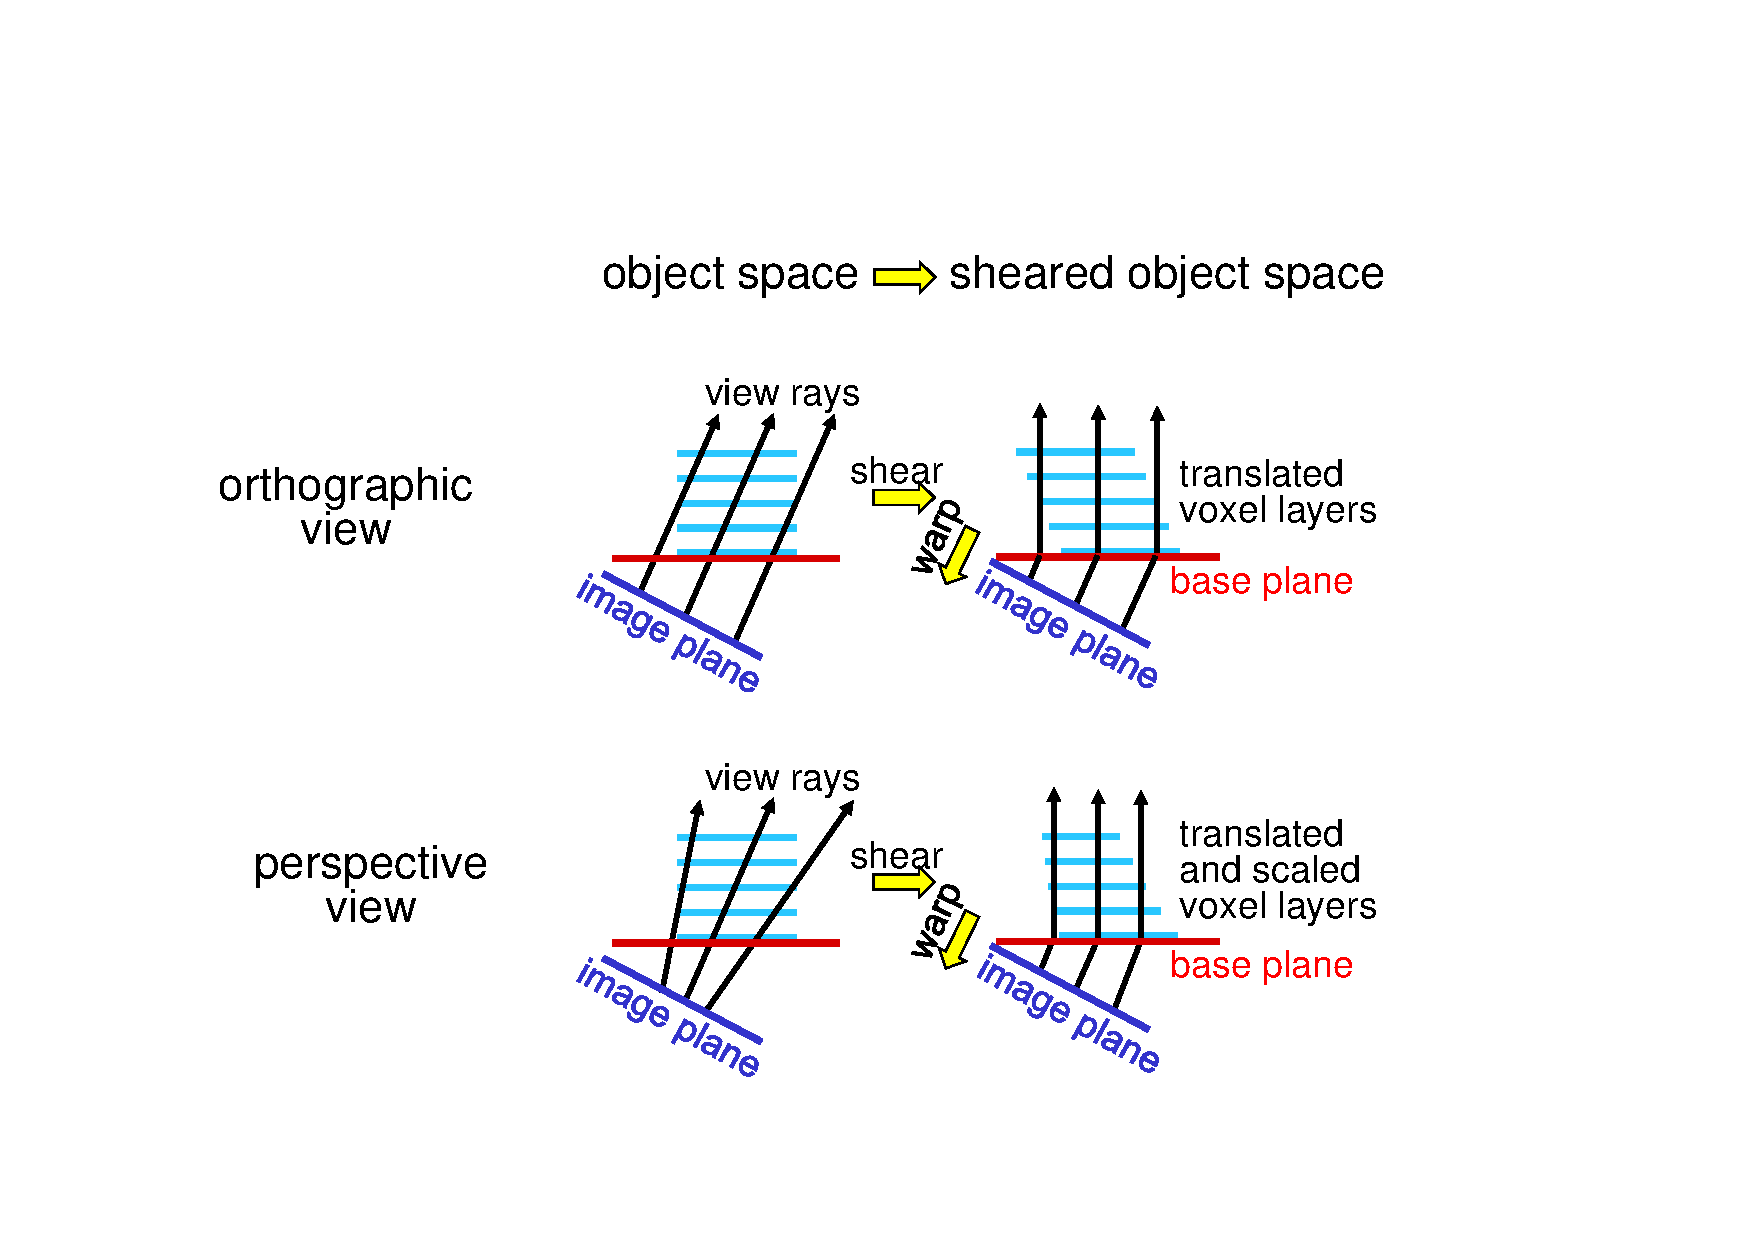
\includegraphics[width=0.8\textwidth]{img/04_shear_warp_overview}
\end{figure}

The \emph{view transformation} is an affine transformation consisting of a rotation and a translation. Ignoring the translation, the $3\times 3$ matrix can be factorised:
\begin{align*}
    M_\text{view} = W\cdot S \cdot P
\end{align*}
where
\begin{itemize}
    \item $P$ is a permutation matrix mapping the base plane to the $xy$ plane.
    \item $S$ is the shear matrix. The \emph{shear} is of the form
        \begin{align*}
            S
            \begin{pmatrix}
                x\\
                y\\
                z
            \end{pmatrix} =
            \begin{pmatrix}
                x\\
                y\\
                z
            \end{pmatrix} + z
            \begin{pmatrix}
                s_x\\
                s_y\\
                0
            \end{pmatrix}.
        \end{align*}
        With $S$ being:
        \begin{align*}
            S =
            \begin{pmatrix}
                1 & 0 & s_x\\
                0 & 1 & s_y\\
                0& 0& 1
            \end{pmatrix}
        \end{align*}
        where $s_x$ and $s_y$ have to be solved for from $M_\text{view}$.
    \item $W$ is the warp matrix. The \emph{warp} is a $3\times 3$ matrix and effectively an affine transformation of the $xy$-plane. The third row of $W$ is irrelevant while two zeros in the third column are required to make the warp independent of $z$.
    \begin{align*}
        W = 
            \begin{pmatrix}
                w_{00} & w_{01} & 0\\
                w_{10} & w_{11} & 0\\
                w_{20} & w_{21} & w_{22}
            \end{pmatrix}
    \end{align*}
\end{itemize}

Assuming for simplicity that $P$ is the identity, we get:
\begin{align*}
    M_\text{view} = \begin{pmatrix}
                         v_{00} & v_{01} & v_{02}\\
                         v_{10} & v_{11} & v_{12}\\
                         v_{20} & v_{21} & v_{22}
                    \end{pmatrix} = W\cdot S = 
            \begin{pmatrix}
                w_{00} & w_{01} & s_x w_{00} + s_y w_{01}\\
                w_{10} & w_{11} & s_x w_{10} + s_y w_{11}\\ 
                w_{20} & w_{21} & s_x w_{20} + s_y w_{21} + w_{22}
            \end{pmatrix}.
\end{align*}
It follows for the warp coefficients $w_{ij} = v_{ij}$ $(j\neq 2)$ and for the shear coefficients:
\begin{align*}
    \begin{pmatrix}
        s_x\\
        s_y 
    \end{pmatrix} =
    \begin{pmatrix}
        v_{00} & v_{01}\\
        v_{10} & v_{11} 
    \end{pmatrix}^{-1}
    \begin{pmatrix}
     v_{02}\\ v_{12}
    \end{pmatrix}
\end{align*}
and for $w_{22}$ (not needed):
\begin{align*}
    w_{22} = -s_x v_{20} -s_yv_{21} + v_{22}.
\end{align*}

If $P$ is not the identity, permuted versions of $S$ and $W$ can be used.

\subsection{Perspective shear warp}
The same factorisation as before can be used. But now \emph{homogeneous coordinates} are used:
\begin{align*}
    M_\text{view} = W\cdot S\cdot P.
\end{align*}
The \emph{shear and scaling} matrix $S$ gets the form
\begin{align*}
  S = 
    \begin{pmatrix}
     1&0&s_x&0\\
     0&1&s_y&0\\
     0&0&1&0\\
     0&0&s_w&1\\
    \end{pmatrix}.
\end{align*}
It does
\begin{itemize}
\item a translation of $x$ by $s_x z$ and of $y$ by $s_y z$ followed by
\item a scaling with ${1\over 1+s_w z}$.
\end{itemize}

The \emph{warp} matrix now is
    \begin{align*}
        W = 
            \begin{pmatrix}
                w_{00} & w_{01} & 0 & w_{03}\\
                w_{10} & w_{11} & 0 & w_{13}\\
                w_{20} & w_{21} & w_{22} & w_{23}\\
                w_{30} & w_{31} & 0 & w_{33}
            \end{pmatrix}.
    \end{align*}
Assuming again that $P$ is the identity we get:
\begin{align*}
    M_\text{view} = \begin{pmatrix}
                         v_{00} & v_{01} & v_{02} & v_{03}\\
                         v_{10} & v_{11} & v_{12} & v_{13}\\
                         v_{20} & v_{21} & v_{22} & v_{23}\\
                         v_{30} & v_{31} & v_{32} & v_{33}\\
                    \end{pmatrix} = W\cdot S = 
            \begin{pmatrix}
                w_{00} & w_{01} & s_x w_{00} + s_y w_{01} + s_w w_{03} & w_{03}\\
                w_{10} & w_{11} & s_x w_{10} + s_y w_{11} + s_w w_{13} & w_{13}\\ 
                w_{20} & w_{21} & s_x w_{20} + s_y w_{21} + w_{22} + + s_w w_{23} & w_{23}\\
                w_{30} & w_{31} & s_x w_{30} + s_y w_{31} + s_w w_{33} & w_{33}\\ 
            \end{pmatrix}.
\end{align*}
It follows that for the warp conditions $w_{ij} = v_{ij}$ with $(j\neq 2)$ holds.
For the shear coefficients:
\begin{align*}
    \begin{pmatrix}
        s_x\\
        s_y\\
        s_w
    \end{pmatrix} =
    \begin{pmatrix}
        v_{00} & v_{01} & v_{03}\\
        v_{10} & v_{11} & v_{13}\\
        v_{30} & v_{31} & v_{33}
    \end{pmatrix}^{-1}
    \begin{pmatrix}
     v_{02}\\ v_{12}\\ v_{32}
    \end{pmatrix}
\end{align*}
and for $w_{22}$ (not needed):
\begin{align*}
    w_{22} = -s_x v_{20} -s_yv_{21}-s_w v_{23} + v_{22}.
\end{align*}

For the shear-warp volume rendering algorithm now works as follows:
\begin{enumerate}
    \item For each voxel layer (parallel to base plane):
        \begin{itemize}
            \item Shear and scale the layer image by multiplying with $S$.
            \item Apply the transfer functions.
        \end{itemize}
    \item Generate intermediate image with $\alpha$ compositing.
    \item Warp the image by multiplying with $W$.
\end{enumerate}

An advantage of this algorithm is that an aliasing filter can be used to prevent undersampling when scaling the image.

\subsection{Object Space versus Image Space}
Comparison of the object space methods introduced and image space methods such as \emph{raycasting}.

Formally both methods are equivalent only the nesting order of the loops is different. Practical differences:
\begin{itemize}
    \item Image space methods with FTB compositing allow early termination.
    \item Object space methods using a framebuffer for intermediate results suffer from quantisation artefacts.
    \item Object space methods can exploit texture mapping hardware and MIPmap textures for antialiasing.
    \item Image space methods would need supersampling in $x$ and $y$ to get antialiasing.
\end{itemize}

\paragraph{Post-classification}
The post-classification can be done directly in the graphics hardware. Using (OpenGL) \emph{depndent texture} (two texture mapping stages):
\begin{figure}[H]
    \centering
    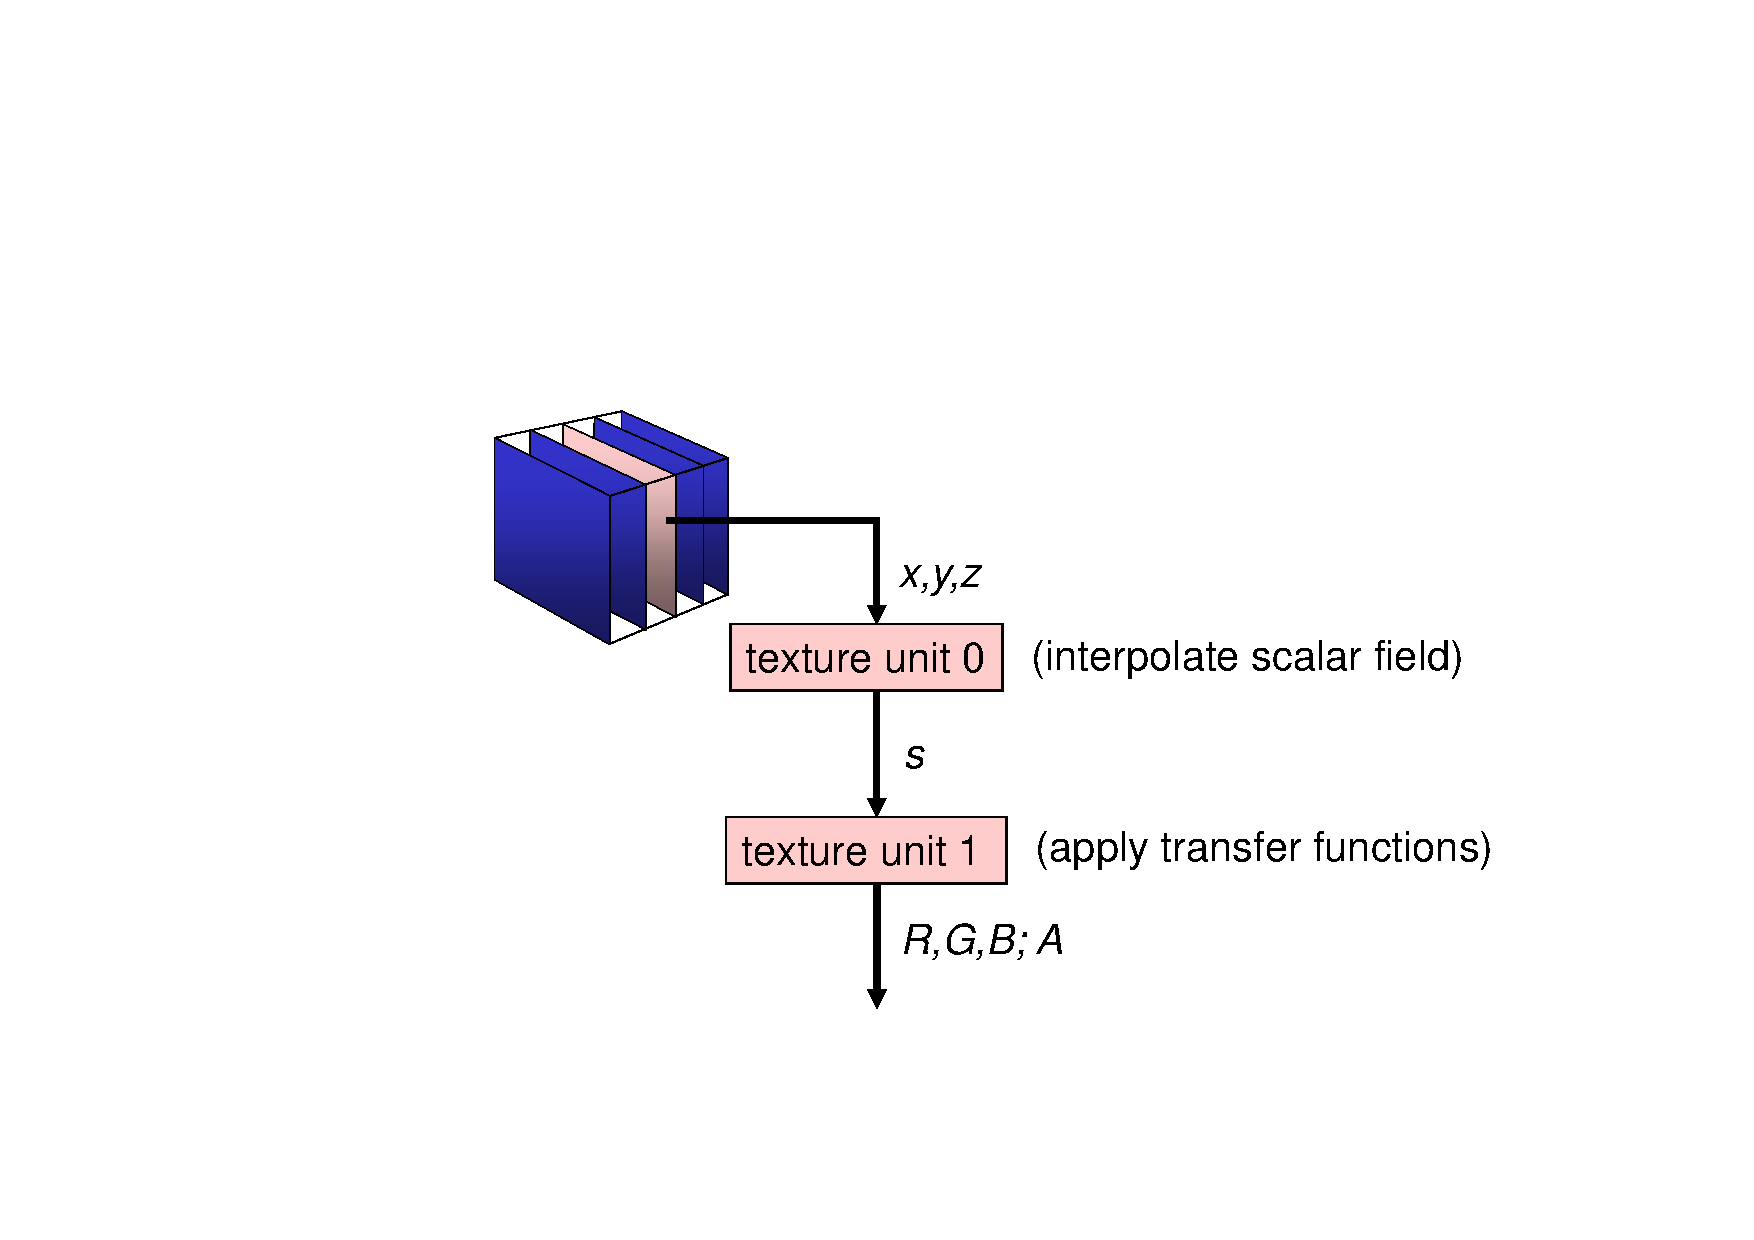
\includegraphics[width=0.6\textwidth]{img/04_object_space_dependent_texture}
\end{figure}

\paragraph{Pre-integration}
It's also possible to pre-integrate in object space:
\begin{itemize}
\item Use \emph{slabs} (space between two slices) and
\item Dependent textures:
    \begin{itemize}
        \item $1^{st}$ stage: Interpolate scalar filed in front and back slice.
        \item $2^{nd}$ stage: Look up integrated transfer function.
    \end{itemize}
\end{itemize}
\begin{figure}[H]
    \centering
    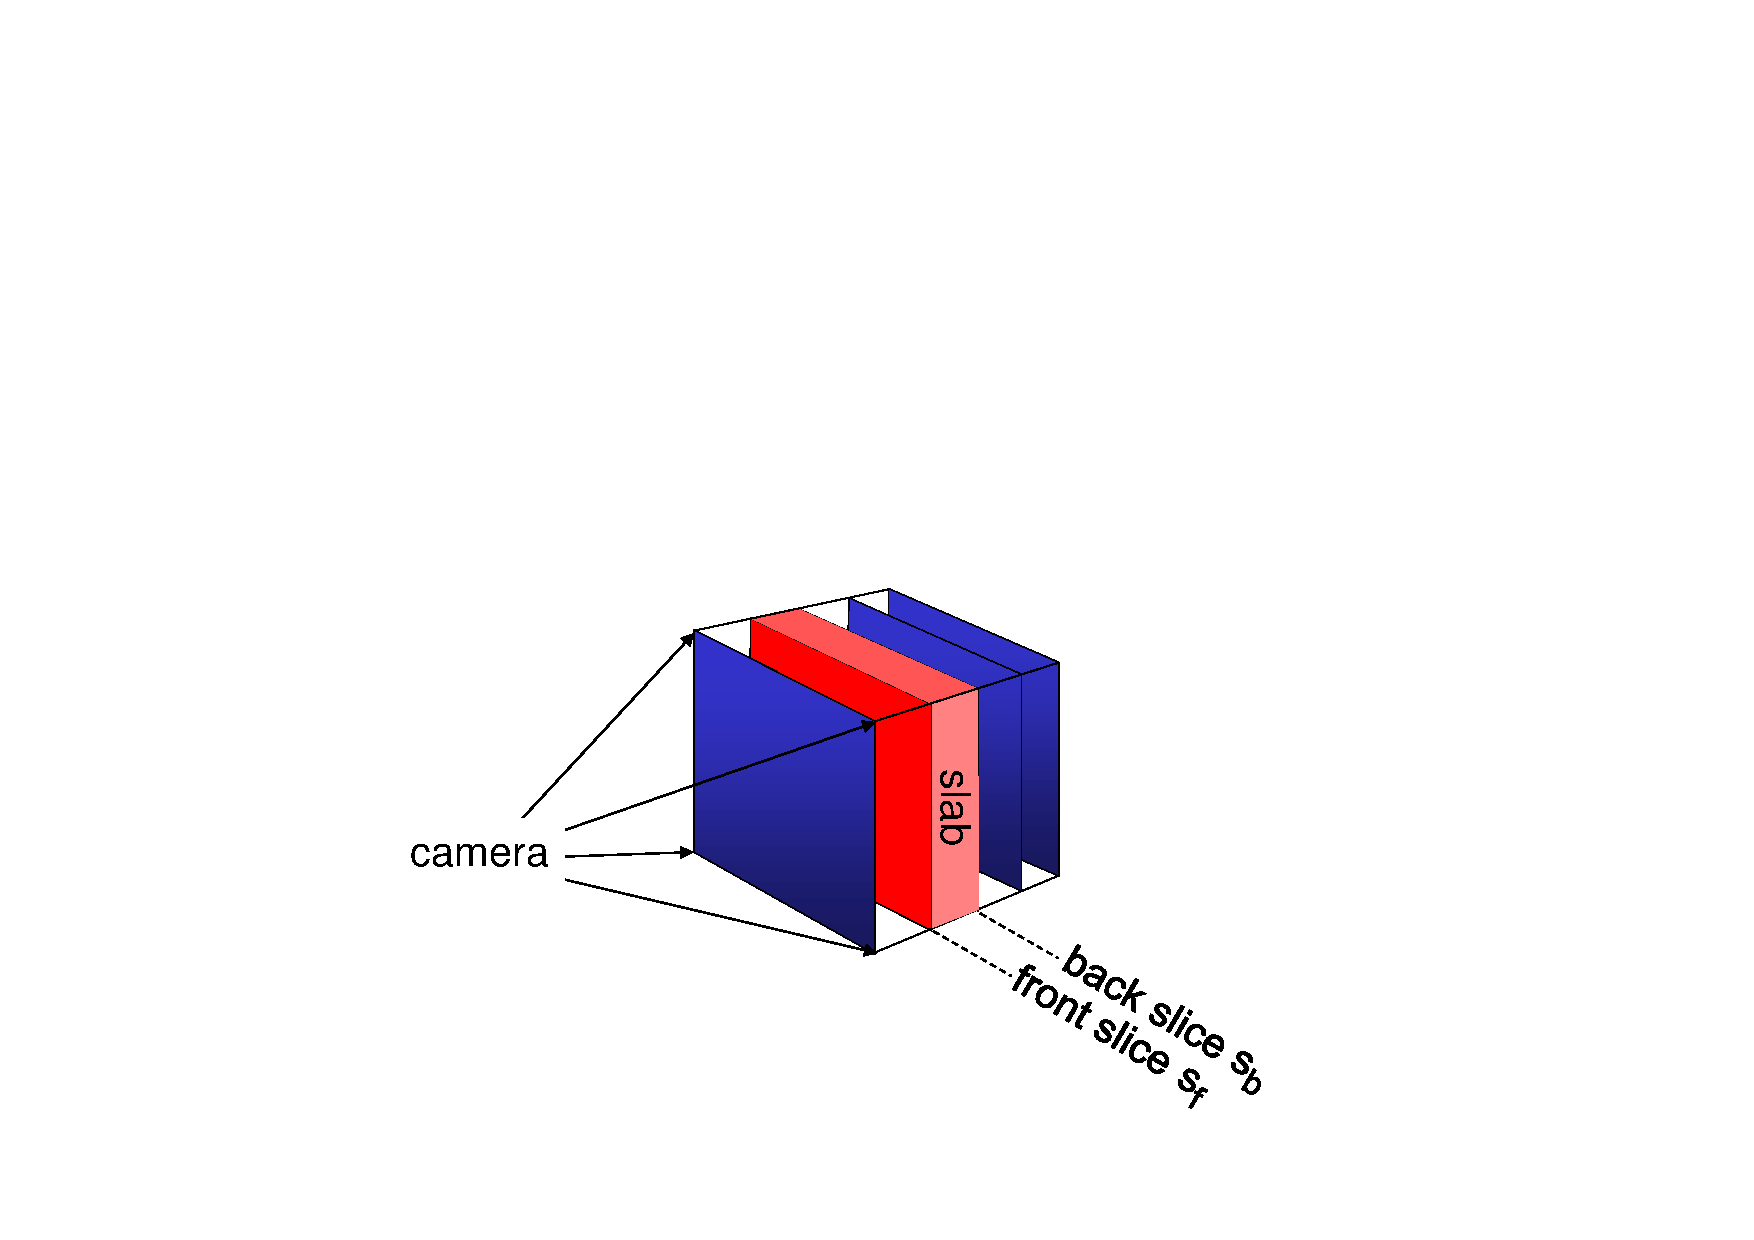
\includegraphics[width=0.6\textwidth]{img/04_object_space_preintegration}
\end{figure}

\subsection{Splatting}

\begin{description}
    \item[Raycasting] "What does \textbf{each} voxel contribute to a given pixel?"
    \item[Splatting] "What does \textbf{a given} voxel contribute to each pixel?"
\end{description}

Algorithm:
\begin{itemize}
    \item Pre-processing:
        \begin{itemize}
            \item For each voxel $x_i$ render (raycast) a field $s(x_i) = \delta_{ij}$.
            \item Store the resulting \emph{footprint} images.
        \end{itemize}
    \item Main loop:
        \begin{itemize}
            \item For each voxel $x_i$ adjust the footprint image to effective TF value.
            \item Do $\alpha$-compositing of all footprint images.
        \end{itemize}
\end{itemize}

Advantages of splatting:
\begin{itemize}
    \item Applicable to structured and unstructured grids.
    \item Other reconstruction filters than trilinear interpolation are possible (for example a sinc filter).
\end{itemize}

\paragraph{Original algorithm} Westover 1990: Orthographic view and uniform grids. All footprints are translations of a template.
\paragraph{Sheet buffer method} Westover 1991:
\begin{itemize}
    \item Blend all footprint images of a voxel layer ("sheet buffer")
    \item Do $\alpha$-compositing of sheet buffers.
\end{itemize}
\paragraph{Elliptical weighted average splatting} (EWA), Zwicker et al. 2001:
\begin{itemize}
    \item Ellipsoidal Gaussians are used as footprints
    \item Perspective view, low-pass filter for antialiasing.
\end{itemize}

\subsection{Cell Projection}
\emph{Projected tetrahedra} (PT) is an object space method for tetrahedral grids [Shirley, Tuchman 1990]. Each (tetrahedral) cell is decomposed into $3$ or $4$ tetrahedra along those edges which are not part of the silhouette.
\begin{figure}[H]
    \centering
    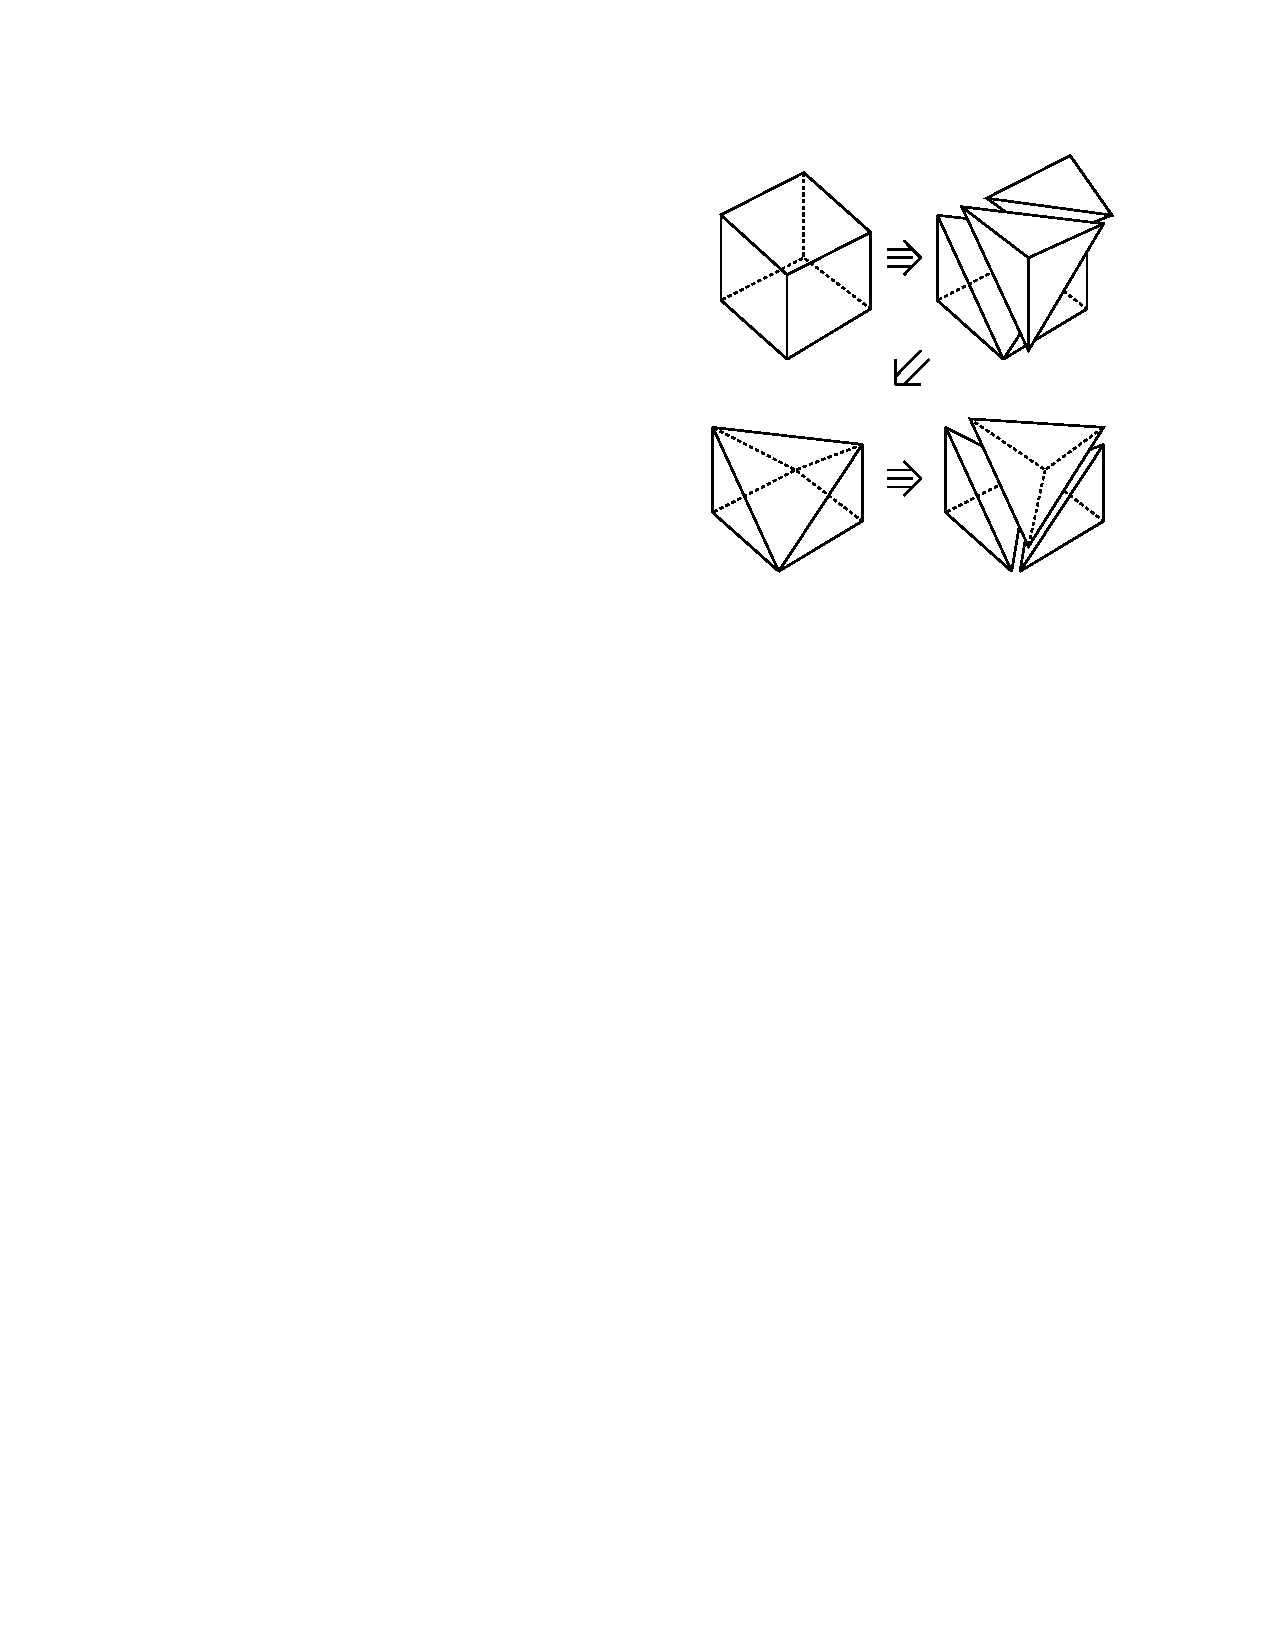
\includegraphics[width=0.6\textwidth]{img/04_cell_based_cropped}
        \caption{Decomposition of a cube into five tetrahedra. Source: A Polygonal Approximation to Direct Scalar Volume Rendering - [Shirley, Tuchmann 1990]}
\end{figure}


Cells are projected to \emph{triangle fans} consisting of
\begin{itemize}
    \item 1 \emph{thick vertex} (projection of the common edge of the tetrahedra)
    \item $3$ or $4$ \emph{thin vertices} (on the silhouette)
\end{itemize}
\begin{figure}[H]
    \centering
    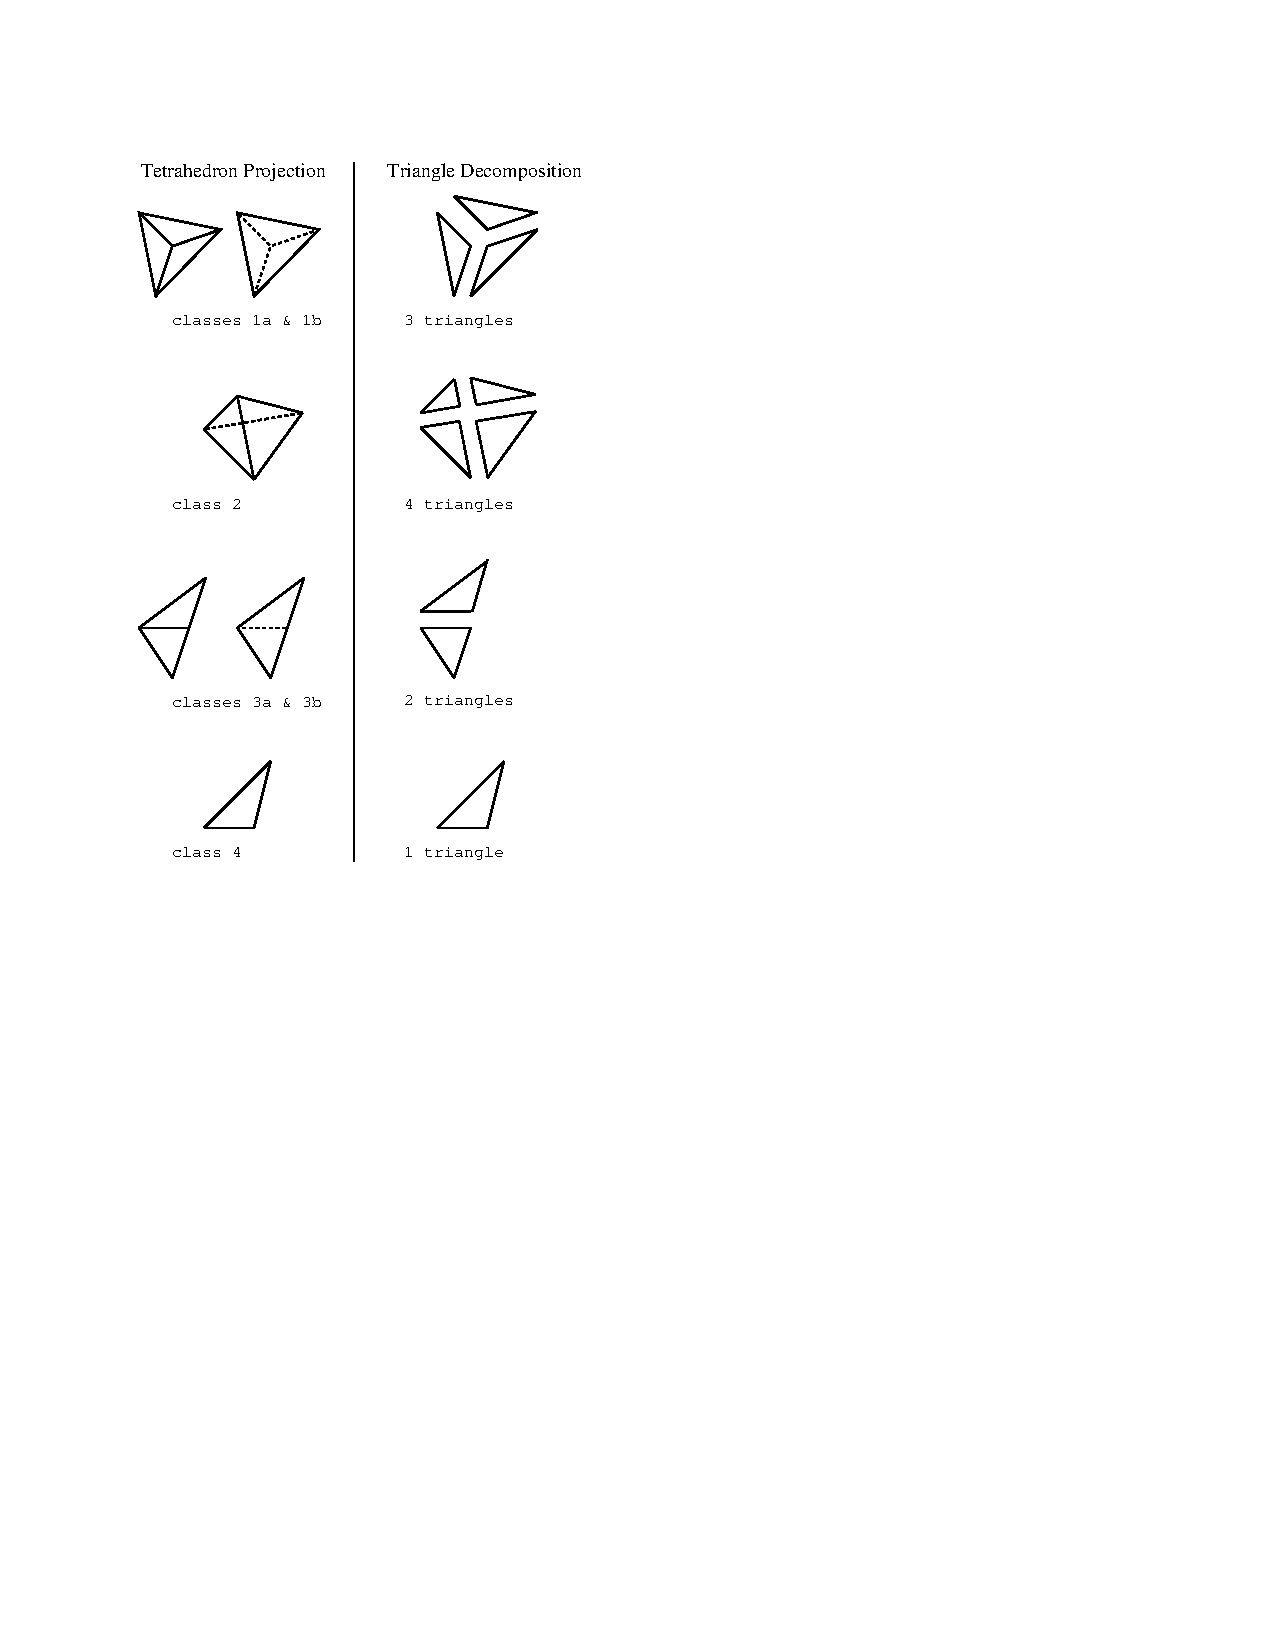
\includegraphics[width=0.6\textwidth]{img/04_cell_based_tetrahedra}
    \caption{Splitting tetrahedra. Source: A Polygonal Approximation to Direct Scalar Volume Rendering - [Shirley, Tuchmann 1990]}
\end{figure}

\paragraph{Original algorithm:} Store \emph{triangle fan} in \emph{space}:
\begin{itemize}
    \item Thin vertices are kept in the \emph{original position}.
    \item The thick vertex is set to the \emph{midpoint} of the projected edge.
\end{itemize}
Advantages:
\begin{itemize}
    \item \emph{Depth test} can be used (allows volume rendering into a scene).
    \item \emph{Viewing direction} and {field-of-view} can be changed (for a fixed camera position) by keeping the projection.
\end{itemize}

\paragraph{Computation of the thick vertex} $\ $
\begin{itemize}
    \item Compute the determinants 
        \begin{align*}
            d_i &= det(x_j, x_k, x_l) &i \in [0,3]
        \end{align*}
        where $x_j$, $x_k$ and $x_l$ are the vertices of the $i^{th}$ face relative to camera position, ordered counter clockwise on the outside of the face.
    \item If the number of positive determinants is 
        \begin{description}
            \item[Odd] Class 1
            \item[Even] Class 2
        \end{description}
    \item Interpolate weights 
\end{itemize}
\paragraph{Painting} The thick and thin vertices are then sent to the graphics card (with supplied texture coordinates). 
\subsubsection{Drawing}
\paragraph{Back-to-front compositing} $\ $
\begin{itemize}
    \item Cells must be depth-sorted $\Rightarrow$ visibility sorting.
    \item Drawing possible without re-sorting on camera turn and zoom.
    \item Depth-test (z-buffer) must be enabled.
    \item Additional (opaque) objects must be rendered before the volumes.
\end{itemize}
\paragraph{Visibility sorting} (MPVO algorithm, Williams 1992):
\begin{itemize}
    \item Generate \emph{partial ordering} of cells based on adjacent pairs.
    \item Break \emph{cycles} (rare, small rendering error, alternative: Split a cell).
    \item Sort the list of \emph{front cells} by distance to centroid (heuristic)
\end{itemize}

\subsubsection{Example: Visualisation of smoke propagation}
For this model we use a simple smoke model which is mostly used in fire protection engineering.
The \emph{absorption} $\tau$ is proportional to $s(x)$ (particle concentration). Which leads a to a simple preintegrated opacity transfer function:
\begin{align*}
    \alpha = 1-\exp\left( 
        - c {\tau_f+\tau_b \over 2}\norm{x_b - x_f}
    \right)
\end{align*}

\subsubsection{Opacities}
When compositing cells with low opacity then opacities are essentially \emph{added}. Adding many very small opacities (e.g. between $[0, 1/255]$) leads to \emph{quantisation artefacts}.
Options to reduce artefacts:
\begin{itemize}
    \item Compositing with $16$ bits
    \item \emph{$\alpha$-dithering} 
        use \emph{randomised rounding} instead of standard rounding:
        \begin{align*}
             x &\rightarrow \lfloor x \rfloor + \left( x - \lfloor x\rfloor \geq \text{rand} \right) &\text{with rand}\in [0,1]
        \end{align*}
        
\end{itemize}

\subsubsection{Hardware-Assisted Visibility Sorting}
HAVS, Silva et al. 2005 is a faster cell projection algorithm:
\begin{itemize}
    \item Requires $4$ RGBA float buffers for storing $7$ pairs of $(s,d)$ per pixel:
        \begin{itemize}
            \item With a scaler field value $s$,
            \item and distance $d$ to camera.
        \end{itemize}
    \item The initial cell sorting is done on the CPU based on the centroids. Which results in a
        \emph{$k$-nearly sorted sequence} with $k\leq 7$.
    \item Main loop: Draw all cell faces from back to front.
    \item Fragment shader:
        \begin{itemize}
            \item Insert $(s,d)$ into buffer
            \item If the buffer is full:
                \begin{itemize}
                    \item Take out furthes pair of $(s,d)$
                    \item Compute thickness of cell behind the pixel:
                        \begin{align*}
                            \Delta d = d-d_\text{old}
                        \end{align*}
                    \item Do a preintegrated TF lookup with $s$, $s_\text{old'}\Delta d$
                    \item Apply $\alpha$ compositing.
                \end{itemize}
        \end{itemize}
\end{itemize}
















\newpage
\section{Vector Field Visualisation}
\begin{itemize}
\item A \emph{static vector field} $v(x)$ is a vector-valued function of space.
\item A \emph{time-dependent vector field} $v(x,t)$ also depends on time.
\end{itemize}
In the case of \emph{velocity fields}, the terms \emph{steady} and \emph{unsteady flow} are used. 

The dimensions of $ x$ and $ v$ are equal, often $2$ or $3$ and we denoted the components by $x,\ y,\ z$ and $u,\ v,\ w$:
    \begin{align*}
         x = (x,\ y,\ z),\qquad v =(u,\ v,\ w).
    \end{align*}
Sometimes a vector field is defined on a surface $x(i,j)$. The vector field is then a function of parameters and time:
    \begin{align*}
        v(i,j,t).
    \end{align*}

\subsection{Visualisation}
An elementary visualisation of a vector field is to \emph{draw arrows}:
\begin{itemize}
    \item At the data points (gird nodes or cell centers), or
    \item at a new (uniform) grids. For 3D fields it's often a 2D slice.
\end{itemize}

Arrows can visualise:
\begin{itemize}
    \item Direction
    \item Relative magnitude (when appropriately scaled(
    \item Time dependency (when animated)
\end{itemize}

\paragraph{Problems} $\ $
\begin{itemize}
    \item It is not clear whether arrows represent vector values at the start point or at the midpoint of the arrow.
    \item Of there exist no satisfactory scaling factors:
        \begin{itemize}
            \item Large scaling: Arrows occlude each other
            \item Small scaling: Direction is not recognisable in some regions
            \item Fixed length: Magnitued information is lost.
        \end{itemize}
\end{itemize}

\subsection{Vector fields as ODEs}
For simplicity, the vector field is now interpreted as \emph{velocity field}. The field $v(x,t)$ describes the connection between location and velocity of a (massless) particle. Which can equivalently be expressed as an \emph{ordinary differential equation}:
\begin{align*}
    \dot x(t) = v(x(t),t).
\end{align*}
This ODE, together with an \emph{initial condition} 
\begin{align*}
    x(t_0) = x_0,
\end{align*}
is a so-called \emph{initial value problem} (IVP). Its solution is the \emph{integral curve} (or \emph{trajectory})
\begin{align*}
    x(t) = x_0 + \int_{t_0}^t v(x(\tau),\tau)d\tau.
\end{align*}

The integral curve is a \emph{pathline} decribing the \emph{path} of a massless \emph{particle} which was released at time $t_0$ at position $x_0$.

Remark: $t<t_0$ is allowed.

For static fields the ODE is \emph{autonomous}:
\begin{align*}
    \dot x (t) = v(x(t))
\end{align*}
and its integral curves
\begin{align*}
    x(t) = x_0 + \int_{t_0}^t v(x(\tau)) d\tau
\end{align*}
are called \emph{field lines} or in the case of velocity fields \emph{streamlines}.

\begin{itemize}
    \item In \emph{static vector fields} pathlines and streamlines are \emph{identical}.
    \item In \emph{time-dependent} vector fields \emph{instantaneous streamlines} can be computed from a "snapshot" at a fixed time $T$ (which is a static vector field):
    \begin{align*}
        v_T (x) = v(x,T).
    \end{align*}
\end{itemize}
In practice time-dependent fields are often given as a dataset per time step. Each dataset is then a snapshot.


Computing streaklines or timelines is more expensive than solving a single IVP.

\subsubsection{Pathlines}
Pathlines are the trajectories that individual fluid particles follow. These can be thought of as "recording" the path of a fluid element in the flow over a certain period. The direction the path takes will be determined by the streamlines of the fluid at each moment in time.\footnote{\url{https://en.wikipedia.org/wiki/Streamlines,_streaklines,_and_pathlines}}

\begin{itemize}
    \item Are physically meaningful
    \item Allow comparison with experiment (observe marked particles)
    \item Are well suited for dynamic visualisation (of particles).
\end{itemize}


\subsubsection{Streamlines}
Streamlines are a family of curves that are instantaneously tangent to the velocity vector of the flow. These show the direction a fluid element will travel in at any point in time.\footnote{\url{https://en.wikipedia.org/wiki/Streamlines,_streaklines,_and_pathlines}}
\begin{itemize}
    \item Are only geometrically but not physically meaningful,
    \item Are easiest to compute (no temporal interpolation, single IVP),
    \item Are better suited for static visualisation (prints),
    \item Don't intersect (under reasonable assumptions)
\end{itemize}

\paragraph{Inputs} $\ $
\begin{itemize}
    \item Static vector field $v(x)$
    \item Seed points with time of release $(x_0, t_0)$
    \item Control Parameters:
        \begin{itemize}
            \item Step size (temporal, spatial or in local coordinates)
            \item Step count limit, time limit, etc...
            \item Order of integration scheme
        \end{itemize}
\end{itemize}
\paragraph{Output} Streamlines as "polylines", with possible attributes.

\paragraph{Preprocessing} $\ $
\begin{itemize}
    \item Set up search structure for point location
    \item For each seed point:
        \begin{itemize}
            \item \emph{Global point location}: \\ Given a point $x$, find the cell containing $x$ and the local coordinates $(\xi, \nu, \zeta)$. \\
            Alternatively if the grid is structured find the computational space coordinates
            \begin{align*}    
                (i+\xi, j+\nu, k+\zeta)
            \end{align*}
            \item If $x$ is not found in a cell then remove the seed point.
        \end{itemize}
        
\end{itemize}
\paragraph{Integration} For each seed point $x$:
\begin{itemize}
\item Interpolate $v$ trilinearly to local coordinates $(\xi, \nu, \zeta)$
\item Do an integration step producing a new point $x'$
\item \emph{Incremental point location}: For position $x'$ find cell and local coordinates $(\xi', \nu', \zeta')$ making use of information (coordinates, local coordinates, cell) of old point $x$.
\end{itemize}
\paragraph{Integration step} Widely used methods:
\begin{itemize}
    \item \emph{Euler}, inaccurate, used only in special speed-optimised techniques:
        \begin{align*}
            x_\text{new} = x+ v(x,t)\cdot \Delta t
        \end{align*}
    \item \emph{Runga-Kutta}, $2^{nd}$ or $4^{th}$ order.  Higher order schemes are often too slow for visualisation. Yeung/Pope 1987 showed that when using standard trilinear interpolation \emph{interpolation errors} dominate \emph{integration errors}.
    \item There are several options for choosing a step size:
        \begin{itemize}
            \item Fixed time stepping $\Delta t$
            \item Fixed spatial step $\Delta s$:
                
                The time step is derive from he spatial step
                    \begin{align*}
                        \Delta t = {\Delta s \over \norm{v(x)}}
                    \end{align*}
                which needs to be corrected iteratively and is used for methods such as LIC.
            \item Adaptive:
                \begin{itemize}
                    \item Adapting to grid resolution (such as cell size)
                    \item Adapting to data variation (Runge-Kutta-Fehlberg method)
                    \item Used for interactive viewing (with zooming)
                \end{itemize}
            \end{itemize}
        
\end{itemize}


\paragraph{Termination criteria} $\ $
\begin{itemize}
    \item Grid boundary reached
    \item Step count limit reached
    \item Optional: Velocity close to zero
    \item Optional: Time limit reached
    \item Optional: Arc length limit reached
\end{itemize}


\subsubsection{Streaklines}
Streaklines are the locus of points of all the fluid particles that have passed continuously through a particular spatial point in the past. Dye steadily injected into the fluid at a fixed point extends along a streakline.

\begin{itemize}
    \item Are physically meaningful
    \item Allow a direct comparison with the experiment (i.e. dye injection)
    \item Are well suited for static and dynamic visualisation
    \item Are a good choice for fast moing vortices
    \item Can be approximated by a set of disconnected particles.
\end{itemize}


Algorithm:
\begin{enumerate}
    \item For time samples $t_0$, $t_1$, $\ldots$, $t_n$ solve the IVP
        \begin{align*}
            \dot x_i (t) &= v(x_i(t), t)\\
             x_i(t_i) &= y
        \end{align*}
    \item Extract the point $x_i(t_n))$
\end{enumerate}

In numerical computation the temporal interval must be \emph{adaptively refined} if two successive particles diverge too much.

\subsubsection{Timelines}
Timelines are the lines formed by a set of fluid particles that were marked at a previous instant in time, creating a line or a curve that is displaced in time as the particles move.


\begin{itemize}
    \item Are physically meaningful
    \item Are well suited for static and dynamic visualisation
    \item Can be approximated by a set of disconnected particles.
\end{itemize}



Algorithm:
\begin{enumerate}
    \item For point samples $y_0$, $y_1$, $\ldots$, $y_n$ on the seed curve solve the IVP:
        \begin{align*}
            \dot x_i (t) &= v(x_i(t),t)\\
            x_i(t_0) = y_i
        \end{align*}
    \item From the integral curve $x_i(t)$ extract the point $x_i(T)$.
    \item Connect these points.
\end{enumerate}
The result is a timeline for time $T$.

In the numerical computation the spatial interval must be \emph{adaptively refined} if two neighbour particles diverge too much.


\subsection{The Stencil Walk algorithm}
Computing the \emph{incremental point location} is nontrivial for curvilinear and unstructured grids.

Buning's \emph{stencil walk} algorithm solves this provlem.

\paragraph{Given}$\ $
\begin{itemize}
    \item Point with coordinates $x$
    \item Cell (as three parameters $(i,j,k)$ or as index $c$ respectively)
    \item Local coordinates $(\xi, \nu, \zeta)$
    \item Coordinates of a new point $x'$
\end{itemize}
\paragraph{Wanted} $\ $
\begin{itemize}
    \item New cell as $(i',j', k')$ or as index $c'$ respectively
    \item New local coordinates $(\xi, \nu, \zeta)$
\end{itemize}

\paragraph{Algorithm}
In a first phase the algorithm find the cell containing $x'$ by iteratively doing:
\begin{itemize}
    \item Take the difference vector $\Delta x = x'-x$
    \item Intersecting the ray $x+t \Delta x$ with the cell boundary giving a $t$ value.
        \begin{itemize}
            \item Linearise the coordinate transform 
                \begin{align*}
                    \phi: (\xi, \nu, \zeta)\mapsto (x,y,z)
                \end{align*}
                in the point $x=(x,y,z)$ by computing the \emph{Jacobian}
                \begin{align*}
                    J={\delta (x,y,z)\over \delta (\xi, \nu, \zeta)} = 
                        \left[
                            {\delta \phi\over \delta \xi} | {\delta \phi\over \delta \nu} | {\delta \phi\over \delta \zeta}
                        \right].
                \end{align*}
            \item Using the \emph{Jacobian} to transform the difference vector $\Delta x = x'-x$ into the local coordinate frame of the cell:
                \begin{align*}
                    (\Delta \xi, \Delta \nu, \Delta \zeta) = J^{-1} \Delta x.
                \end{align*}
            \item Find the intersection of the ray
                \begin{align*}
                    (\xi, \nu, \zeta) + t(\Delta \xi, \Delta \nu, \Delta \zeta)
                \end{align*}
                with the cell boundary having the equations:
                    \begin{align}
                         \xi, \nu, \zeta &= 0\\
                         \xi, \nu, \zeta &= 1 &\text{for hex cell}\\
                         \xi + \nu + \zeta &= 1 &\text{for tet cell}\\
                         0 \leq \xi, \nu, \zeta &\geq 1 &\text{inequalities}
                    \end{align}

        \end{itemize}
        Due to linearisation the point is not exact and in most cases the correct neighbour cell is found.
    \item If $t\geq 1$ the point $x'$ lies in the current cell and iteration can be stopped.
    \item Otherwise move to the neighbour cell adjacent at the intersection point
    \item If no such cell exists terminate with failure
    \item Set the \emph{cell centroid} as the new $x$ for the next iteration.
\end{itemize}


\subsubsection{Problems}
If the cells are sufficiently skewed the algorithm can walk away from the target cell.
\begin{figure}[H]
    \centering
    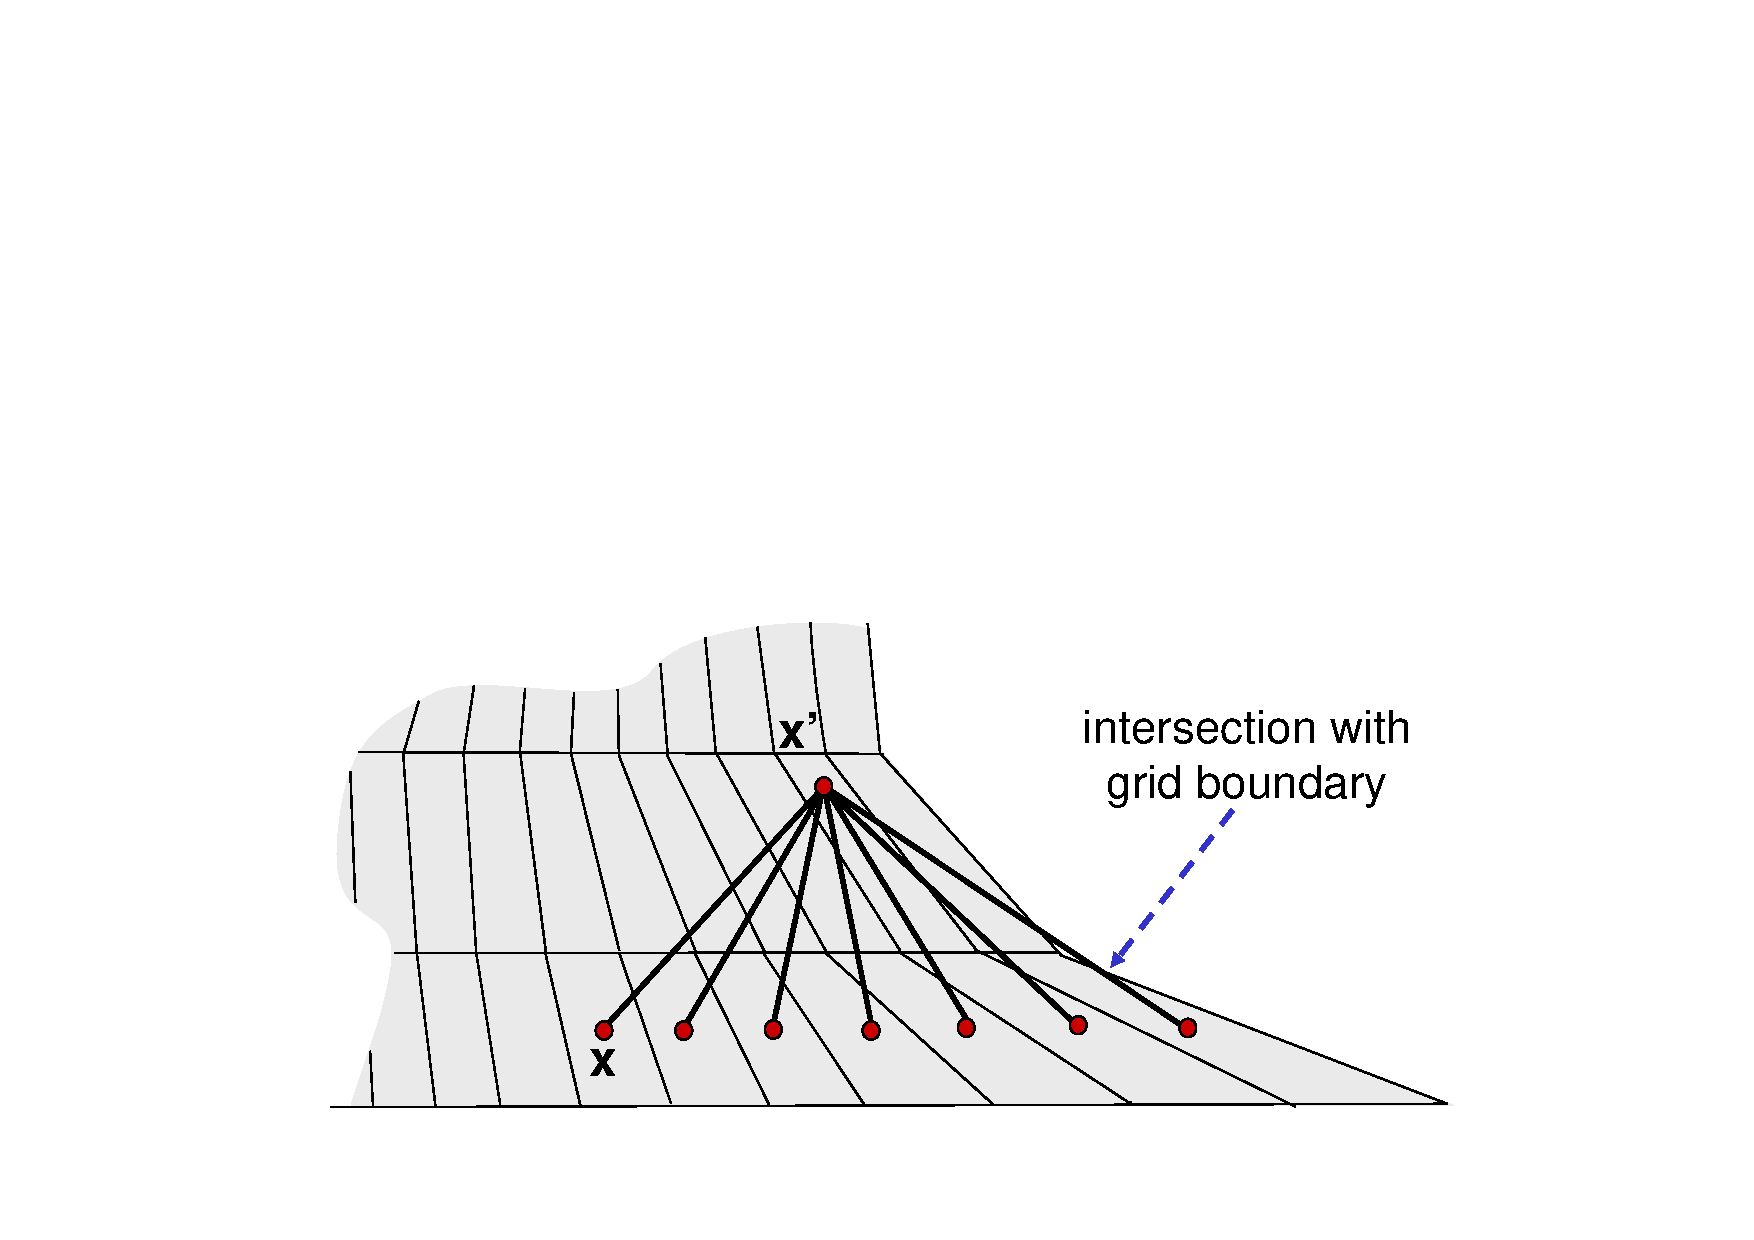
\includegraphics[width=0.8\textwidth]{img/05_stencil_walk_problems}
\end{figure}

This problem can be solved with a \emph{modification} of the algorithm:
\begin{itemize}
    \item Keep ray $(x,x')$ unchanged
    \item New Problem: Cell faces of the type \emph{quadrangle} (nonplanar!) can be intersected \emph{twice}!
    \begin{figure}[H]
    \centering
    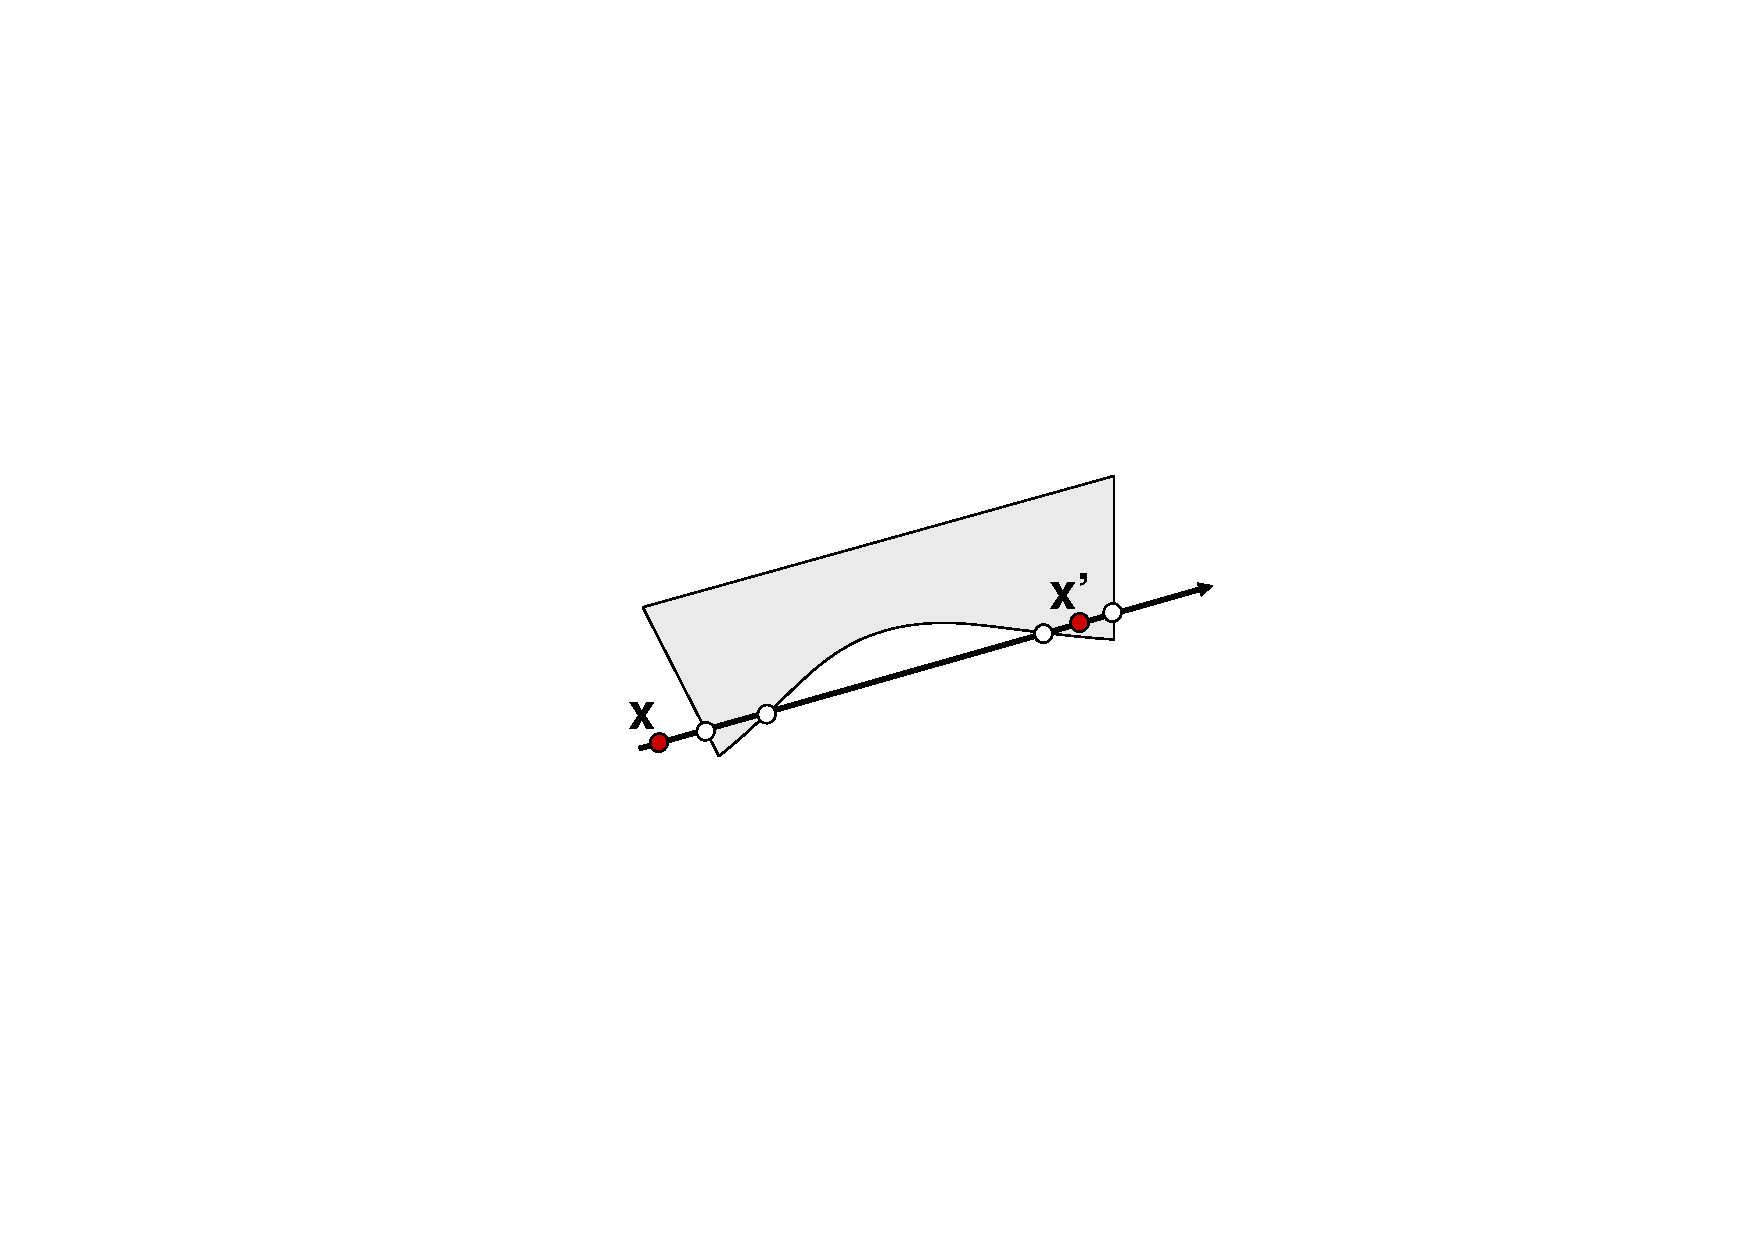
\includegraphics[width=0.8\textwidth]{img/05_stencil_walk_improved}
    \end{figure}
    Therefore \emph{exact} intersection points of the ray with bilinear surface patches must be calculated:
\end{itemize}

\paragraph{Exact intersection calculation} If the quadrangle is \emph{nonplanar} the four corners $P_0$, $P_1$, $P_2$, $P_3$ can be mapped to:
\begin{align*}
    \tilde P_0 &= (0,0,0)\\
    \tilde P_1 &= (1,0,0)\\
    \tilde P_2 &= (1,1,1)\\
    \tilde P_3 &= (0,1,0)
\end{align*}
by the \emph{affine transformation}
\begin{align*}
    \tilde x = (\tilde P_1 | \tilde P_2 | \tilde P_3) (P_1|P_2|P_3)^{-1} (x-P_0).
\end{align*}
The bilinear surface containing $P_0'$, $P_1'$, $P_2'$ and $P_3'$ is the \emph{hyperbolic paraboloid}
\begin{align*}
    z = xy.
\end{align*}
Inserting the transformed view ray $\tilde x + t\Delta \tilde x$ leads to a quadratic equation for $t$:
\begin{align*}
    (\tilde z + t\Delta \tilde z) = (\tilde x+t\Delta \tilde x)(\tilde y + t\Delta \tilde y).
\end{align*}
If real solutions with $0<t<1$ exist the intersection points $(\tilde x_i, \tilde y_i, \tilde z_i)$ are computed and transformed back.

In the second phase the stencil walk algorithm computes the local coordinates of the point in the cell known to contain it. The local coordinates are the inverse of the coordinate function:
\begin{align*}
    \phi: (\xi, \nu,\zeta)\mapsto (x,y,z)
\end{align*}
evaluate at the given point 
\begin{align*}
 x= (x,y,z).
\end{align*}
However, the trilinear function $\pi$ is a cubic polynomial and its inverse is a sixth-degree polynomial. Hence the problem needs to be solved with Newton's method.

\subsection{Global Point Location}
Global point location is more expensive than the stencil walk algorithm.

Many methods trade in safety for efficiency. A few methods are:
\begin{enumerate}
\item Search for the point in every grid cell using Newton's Method.

Hypothetic "brute force" method. Safe.
\item Buning's method.

Do incremental point location starting from a boundary cell. \textbf{Problem}:

Node $(O)$ nearest to given point $(X)$ is not necessarily adjacent to the cell containing it. Furthermore the straight line between the two points can leave the grid.
    \begin{figure}[H]
        \centering
        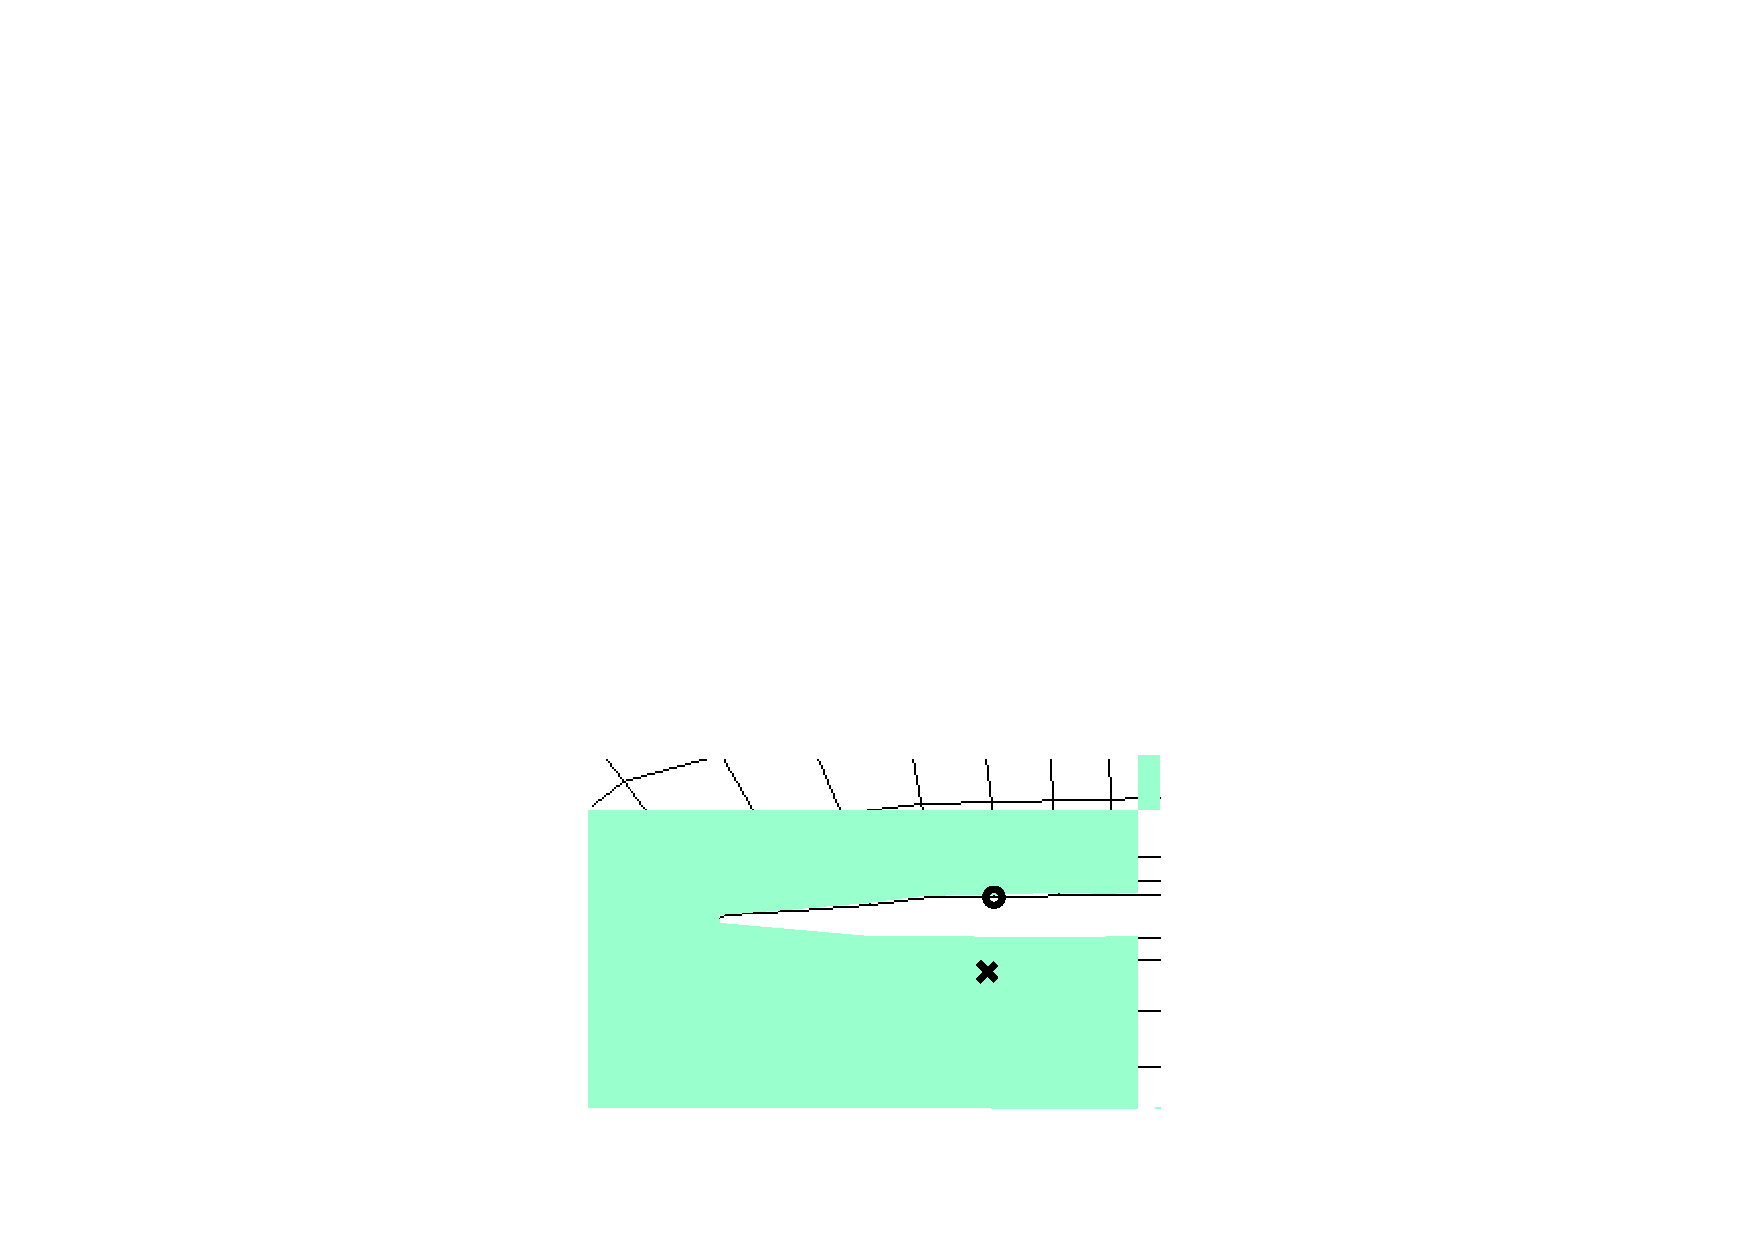
\includegraphics[width=0.5\textwidth]{img/05_bunings_method}
    \end{figure}
    
    Bunings method is safe if incremental search is repeated with a different boundary cell as long as the point is not found. Instead of using all boundary cells, precompute a subset of boundary cells to guarantee to find all points within the grid.
\item Incremental point location starting from a node near the grid center.

Simple method. Only safe for \emph{star-shaped} grids.
\item Search structure based.

Efficient methods use a search structure such as a uniform grid, octrees or kd-trees for nodes or cell centers:
\begin{itemize}
    \item When a point query is not sufficient a \emph{range query} is need with a range determined by the cell size.
    \item Problem: Cells can have extreme aspect ratios (especially from CFD).
\end{itemize}
\item Bounding box hierarchy

Use a bounding box hierarchy for a recursively subdivided grid. Efficient and safe method and easy for structured grids.

More preprocessing is required for unstructured grids (cell tree, Garth 2010)
\end{enumerate}

\subsection{Computational Space Streamline Integration}
In structured grids \emph{point location} can be \emph{avoided} by using a different approach:

Integration can be done in computational space $\mathcal C$ instead of physical space $\mathcal P$. This requires a modification of the integration algorithm:

\begin{itemize}
    \item \emph{Before} the integration step:
    
    Transform the \emph{velocity} $v(x)$ to $\mathcal C$ by multiplying with $J^{-1}$
    \item \emph{After} the integration step:
    
    This step is only required if graphical output of this step is needed. Transform the new \emph{position}
    \begin{align*}
         x= (i+\xi, j+\nu, k+\zeta)
    \end{align*}
    to $\mathcal P$ by trilinear interpolation.
\end{itemize}

Main problem of the integration in $\mathcal C$:
\begin{itemize}
    \item The ordinate function
    \begin{align*}
        \phi: (i+\xi,j+\nu, k+\zeta) \mapsto (x,y,z)
    \end{align*}
    is only $C^0$ continuous at cell boundaries.
    \item Therefore $J$ is discontinous.
    
    \item Example (Sadarjoen 1994): Four cells with a constant velocity field.
    \begin{figure}[H]
        \centering
        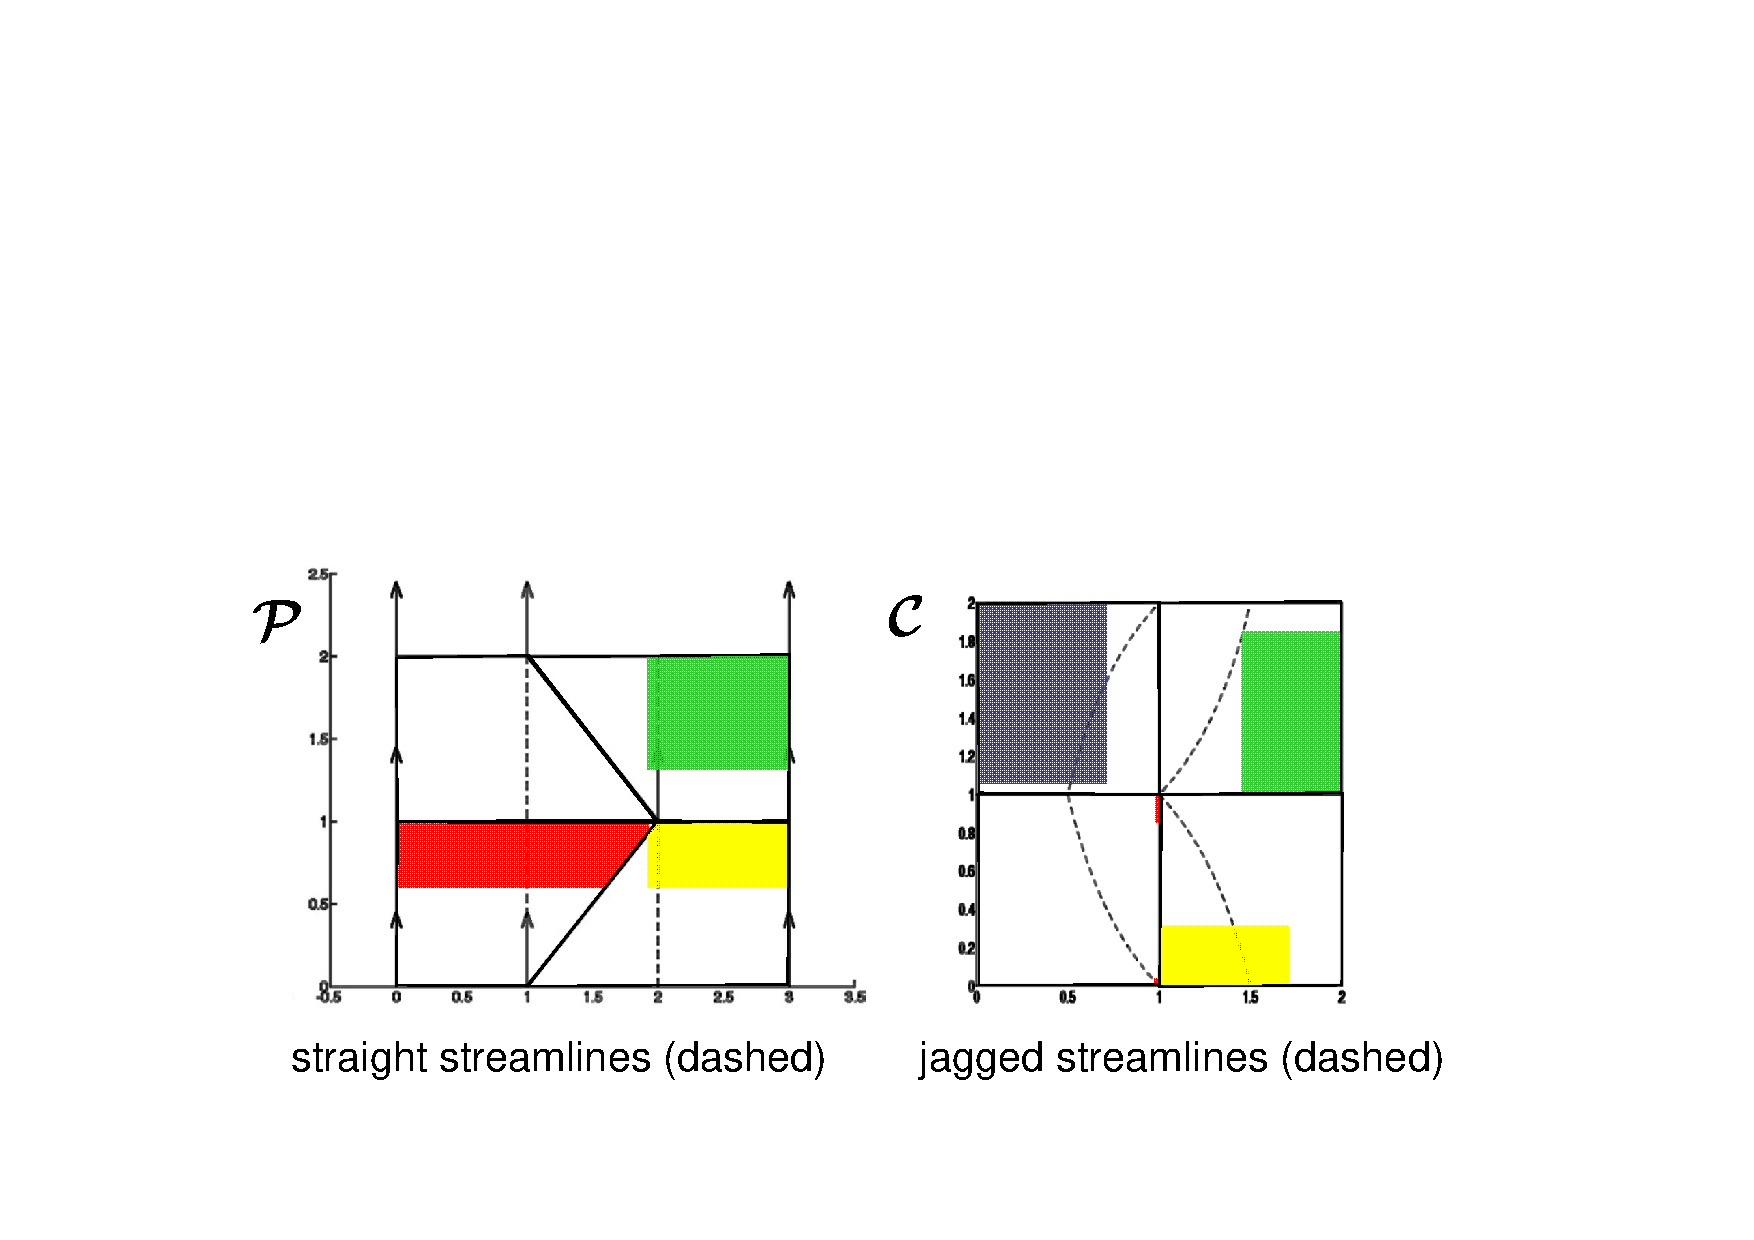
\includegraphics[width=0.6\textwidth]{img/05_cspace_integration_problem}
    \end{figure}
\end{itemize}

Two sources of error:
\begin{itemize}
    \item Integration steps across cell boundaries.
    
    This can be avoided by shortening such steps.
    
    \item Use of a (precomputed) single transformed field vector by node. 
    
    Can be fixed by transforming all eight vectors of a cell on the fly when entering a new cell.
\end{itemize}

The main advantage of integration in $\mathcal C$ is its algorithmic simplicity. But if it's done correctly (avoiding the errors above) it can be slower than an integration in $\mathcal P$.

\subsection{Skin Friction Lines}
Velocity fields of fluid flow can have grid boundaries which are walls (i.e. solid material surfaces). At walls the velocity vector is usually zero as a result of the no-slip boundary condition.
Therefore a derived vector field is often used: The \emph{wall shear stress}:
\begin{align*}
    \tau_w = \mu{\delta v_w\over \delta s},
\end{align*}
can be obtained as the limit of the wall-parallel velocity component $v_w$ divided by the wall distances $s$ and multiplied with the \emph{dynamic viscosity} $\mu$ (material constant). This limit is typically nonzero except at isolated points.

Streamlines of $\tau_w$ are called \emph{skin friction lines}. They are an example of a vector field defined on a surface in $3$-space.

\subsection{Streamline Placement}
The problems of visualisation by streamlines:
\begin{itemize}
    \item Dependency on seed points,
    \item and the density of streamlines can be largely inhomogogeneous.
\end{itemize}

\paragraph{Solution} Automatically optimise choice of seed points.
\begin{enumerate}
 \item \emph{Streamlets} (short streamline segments)
     
     The length is proportional to the velocity magnitude (obtained automatically by using a fixed integration time).
     
     Start with a uniform grid and make spacing roughy even by locally adapting (displacing, inserting, removing) seeds.

Typical use: Displaying weather maps

\item Algorithm by Turk and Bank (longer streamlines):

Objective: Create a streamline image which when low-pass filtered has a uniform grey level.

Optimise seed positions and integration lengths.

Operations:
\begin{itemize}
    \item Insert
    \item Delete
    \item Move
    \item Lengthen
    \item Shorten
\end{itemize}
Apply operations either randomly or based on oracles.

\end{enumerate}


\subsection{Streamsurfaces}
Definition: Union of streamlines seeded densly on a curve. 

Advantage for visualisation:
Structured, better spatial perception.

Naive algorithm:
\begin{itemize}
    \item Start integration at discrete samples on the seed curve.
    \item Conncect points of equal integration time resulting in a quad mesh.
\end{itemize}
This fails if streamlines diverge or grow at largely different speeds.
\begin{figure}[H]
    \centering
    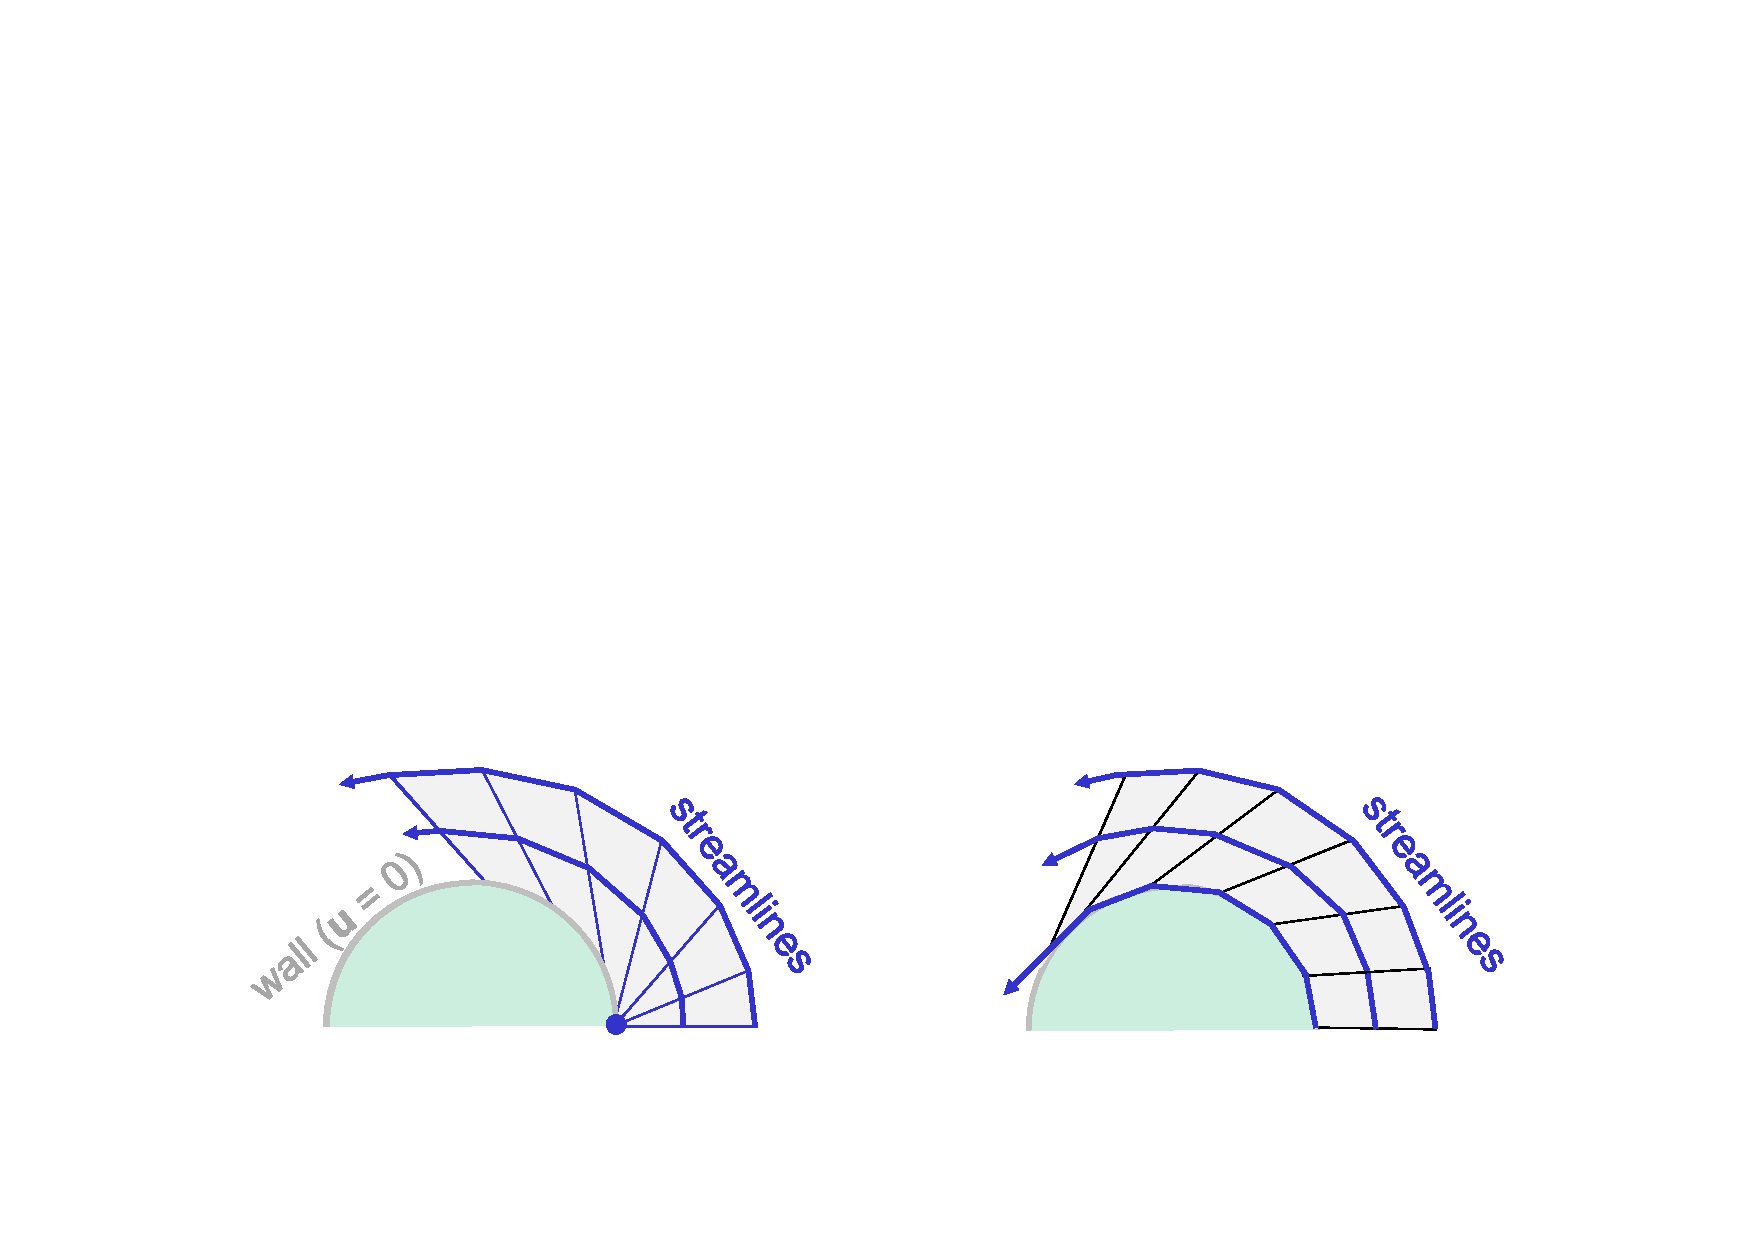
\includegraphics[width=0.8\textwidth]{img/05_streamsurfaces}
\end{figure}

\paragraph{Hultquist's algorithm} solves this problem of speed differences by \emph{optimised triangulation}: Of two possible connections choose the one which is closer to orthogonal (sic) to both streamlines.
\begin{figure}[H]
    \centering
    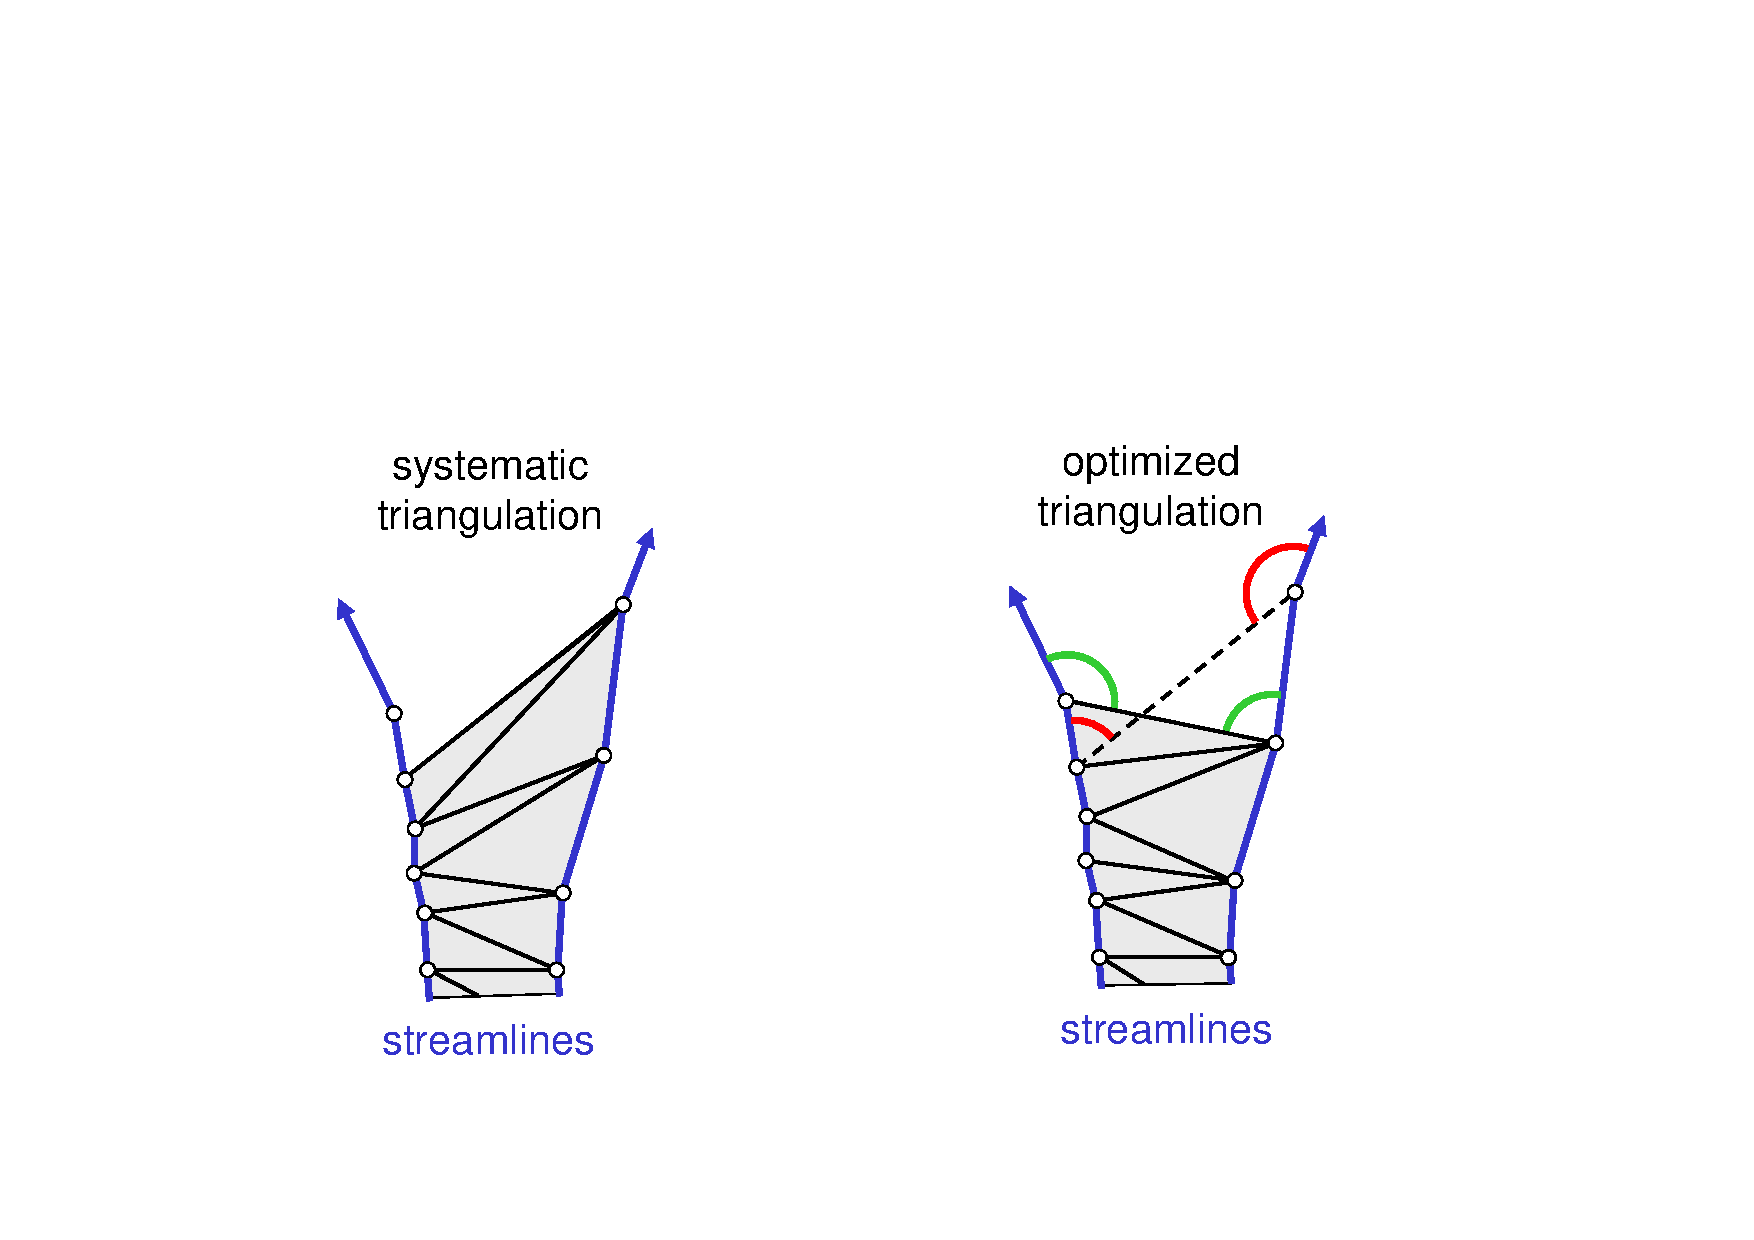
\includegraphics[width=0.8\textwidth]{img/05_hultquist}
\end{figure}
The problem of divergence or convergence is solved by \emph{inserting} or \emph{terminating streamlines}.
\begin{figure}[H]
    \centering
    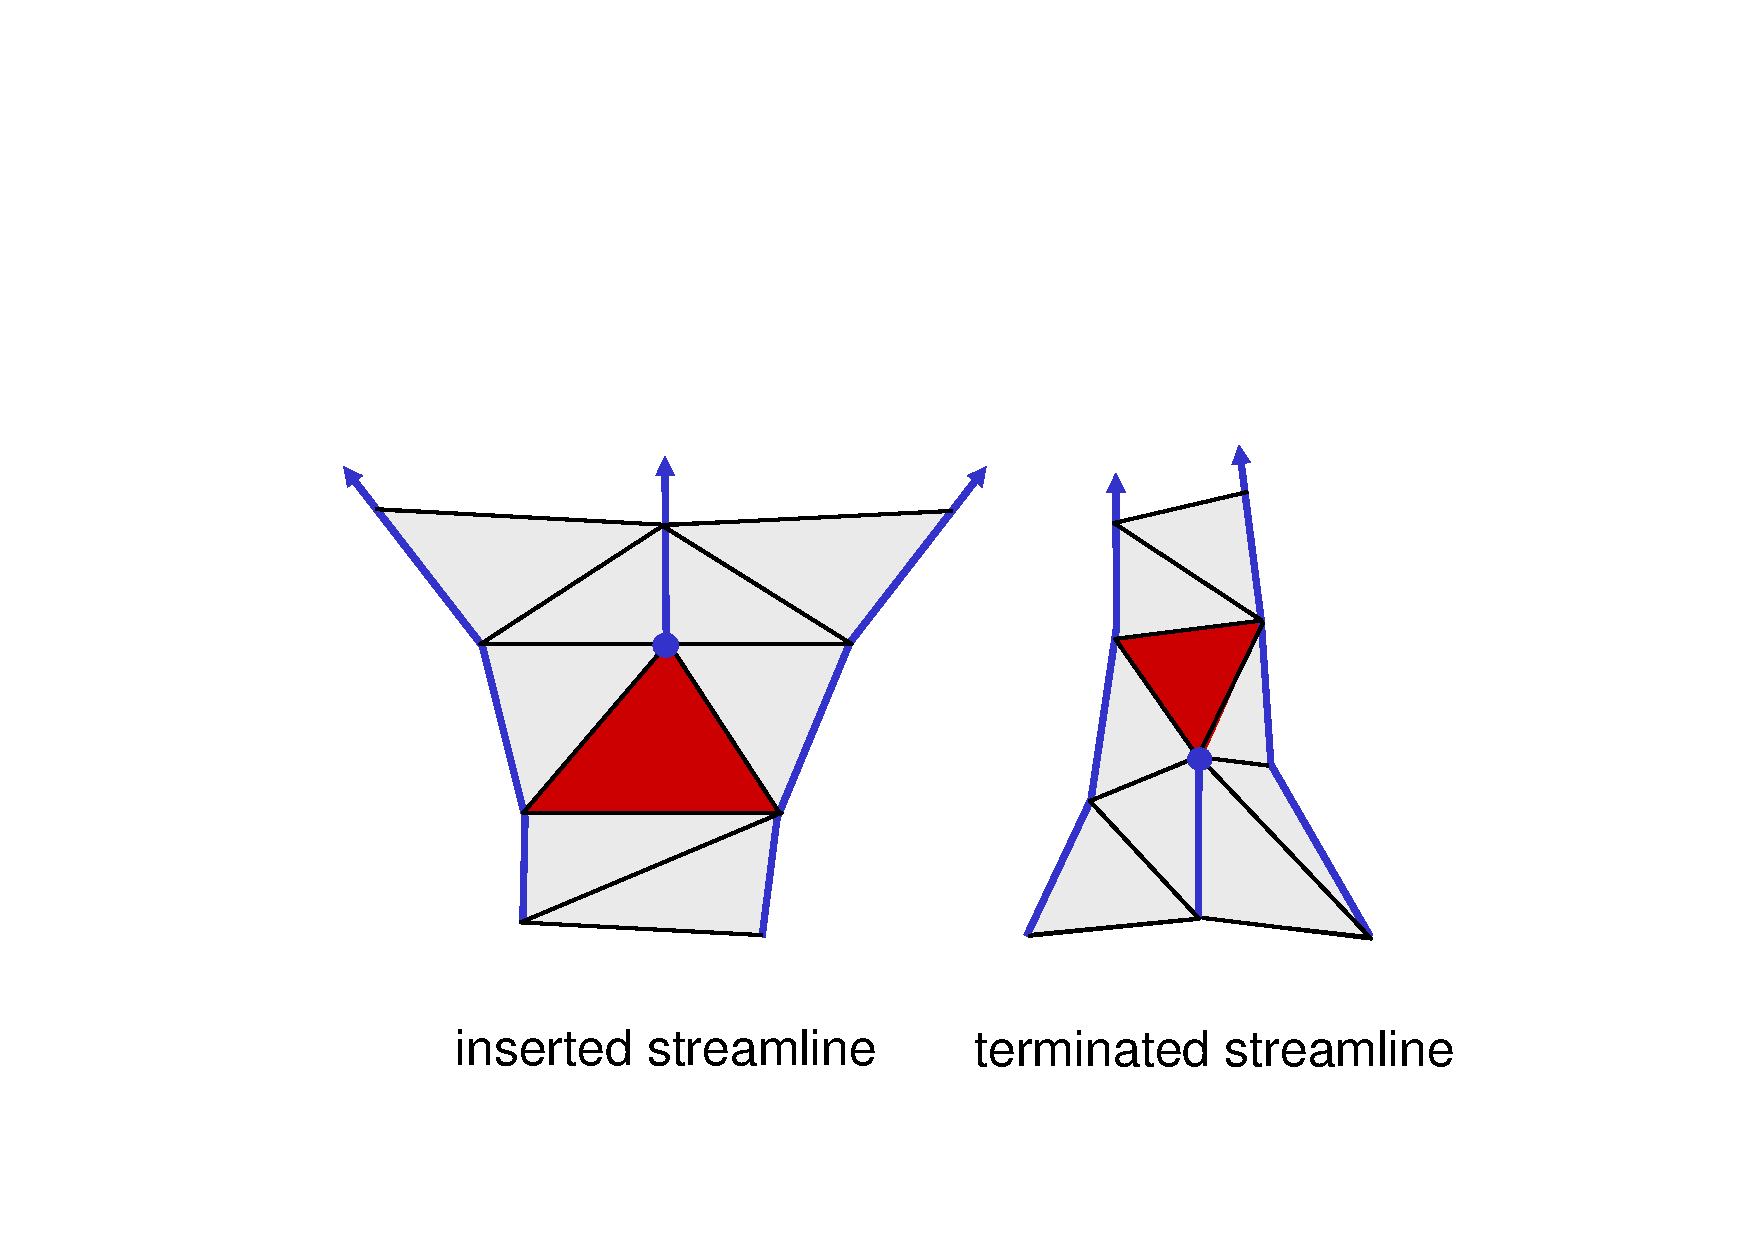
\includegraphics[width=0.8\textwidth]{img/05_hultquist_divergence}
\end{figure}

Also use hermite interpolation for streamsurface patches:
\begin{figure}[H]
    \centering
    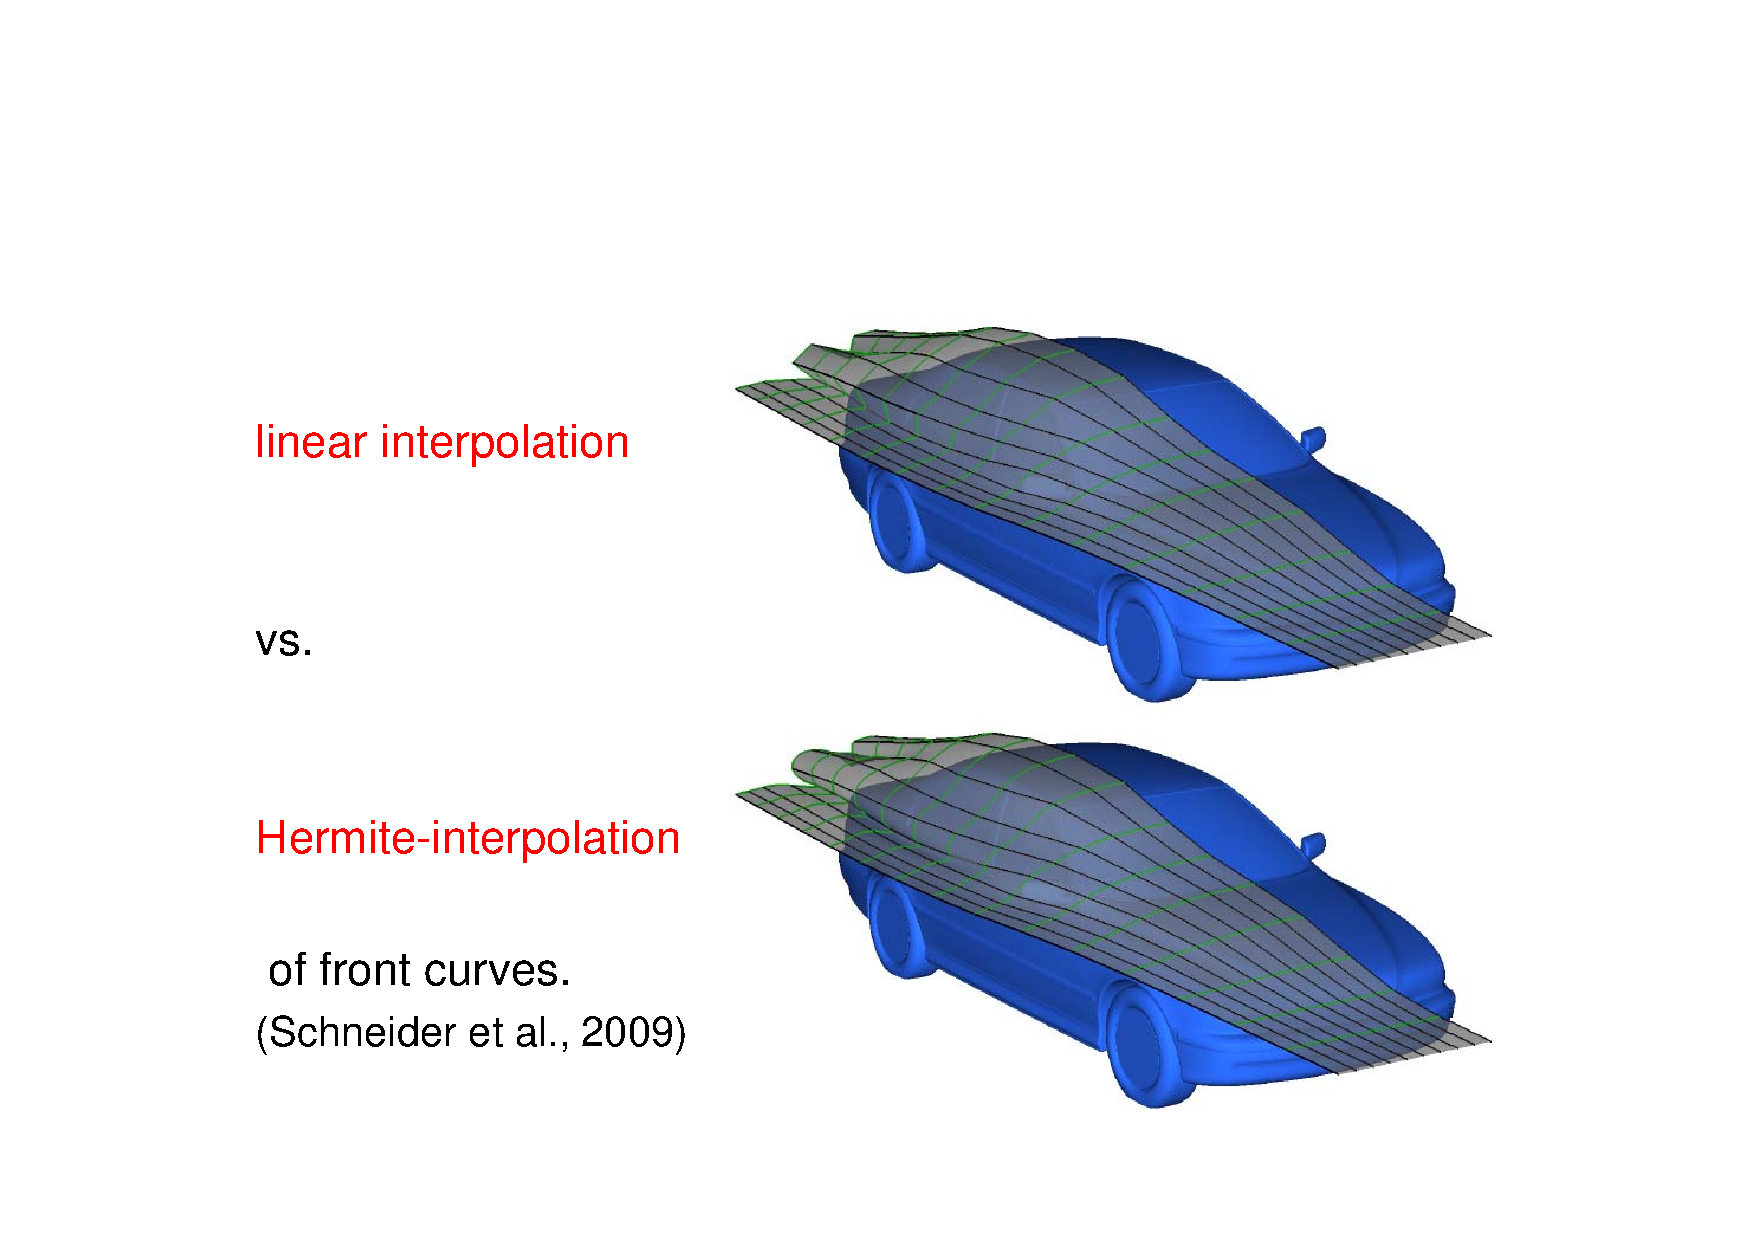
\includegraphics[width=0.8\textwidth]{img/05_hultquist_interpolation}
\end{figure}

\subsection{Streak Surfaces}
Stream lines in 3D on a fully adaptive triangle mesh.











\newpage
\section{Texture Advection}
Motivation: \emph{Dense} visualisation of vector fields without any seed points.

\begin{description}
\item Methods for \emph{static} fields:
    
    LIC - Line integral convolution (Cabral/Leedom 1993)
\item Methods for \emph{time-dependent} fields:
    \begin{itemize}
        \item LEA - Lagrangian-Eulerian Advection (Jobard et al. 2001)
        \item IBFV - Image-Based Flow VIs (van Wijk 2002)
    \end{itemize}
\item Methods for vector fields \emph{on surfaces}
    \begin{itemize}
        \item IBFVS - IBV for Surfaces
        \item ISA - Image-Space Advection (Laramee 2003)
    \end{itemize}

\end{description}

\subsection{Line Integral Convolution}
Line integral convolution (LIC) is a family of 10+ variants. The original method by Cabral and Leedom assumes 2D vector fields on rectilinear grids.

Basic idea:
\begin{enumerate}
    \item Generate a grey level image of random pixels at the desired resolution.
    \item Compute forward and backward streamline segments of fixed arc length for all pixels.
    \item Sample the random image along the streamline and compute the average (i.e. convolve with a box filter).
    \item Use the computed values as the pixels of the output image.
    \item Stretch the range of the output image.
\end{enumerate}

LIC images can be combined with a colour coding of a scalar field:
\begin{description}
\item in \emph{HSV} space:
    \begin{description}
        \item hue: Scalar field
        \item saturation: 1
        \item value: LIC
    \end{description}
\item in \emph{HLS} space:
    \begin{description}
        \item hue: scalar field
        \item lightness: LIC
        \item saturation: 1
    \end{description}
\end{description}

\paragraph{The Fast LIC method} (Stalling) is an order of magnitude faster by reusing parts of streamlines where possible. Fast LIC is the basis of most the newer LIC methods.

\paragraph{LIC for unstructured grids} (Battke) uses a \emph{procedural} 3D random image. For each triangle a LIC image is computed separately and displayed as a separate texture map.

This method can also be used for \emph{vector fields on surfaces}.

\paragraph{LIC method for curvilinear grids} (Forsell). Generate a LIC in computational space $\mathcal C$ and use it as a texture map for the grid in physical space $\mathcal P$.

Problems of this approach: If parameters lines are not smooth and cell sizes have a large variation the then resulting image might show artefacts.

\paragraph{Animated LIC} The LIC of static vector fields can be easily animated to show the relative velocity magnitueds:
\begin{itemize}
    \item Use samples at constant \emph{time steps}
    \item Replace the box filter by \emph{sinusodial} filter with exactly one period.
    \item Shift the kernel \emph{backward} in steps of one sample.
\end{itemize}
This results in the texture moving forward.

\paragraph{3D LIC} LIC can be computed easily in 3D but the result is a 3D image. Rendering options:
\begin{description}
    \item Isosurfaces: NO
        
        Sensitive to noise, LIC is a near worst case!
        
    \item Direct volume rendering: Yes
\end{description}

\subsection{Multi-Layer Flow Textures}

Multi-Layer LIC-like textures (Carnecky 2012) require:
\begin{itemize}
    \item Multi-Layer screen-space data structure ("illustration buffer")
    \item Procedural 3D noise texture with constant screen-space frequency
    \item Anisotropic diffusion to obtain flow aligned texture. 
\end{itemize}

\subsection{Lagrangian-Eulerian Advection}
Dynamic behaviour can be expressed in either Eulerian or Lagrangian formulation:
\begin{description}
\item[Eulerian] or \emph{grid-based}:

Fields are given at grid nodes
\item[Lagrangian] or \emph{particle-based}: 

A set of particles is advected by the velocity field $v(x,t)$, other fields are given at particle positions.
\end{description}

The temporal change of a function $f(x,t($ \emph{while following a particle} is expressed by the \emph{material derivative} (or convective derivative):
\begin{align*}
    {Df(x,t)\over Dt} = {\delta f(x,t)\over \delta t} + \Delta f(x,t)\cdot v(x,t)
\end{align*}


\subsubsection{Lagrangian-Eulerian Advection for Vector Field Visualisation}
The LEA method for vector field visualisation (Jobard 2011) uses \emph{one particle per cell}:

Initialise a white noise texture (same as for LIC).
\begin{description}
\item For each time step do:
    \begin{description}
        \item For each particle do:
            \begin{itemize}
                \item Integrate \emph{backward} pathline segment giving a new \emph{texel value} for the cell.
                \item Integrate \emph{forward} pathline segemtn giving the new \emph{particle position} in the same cell (local coordinates modulo 1).
            \end{itemize}

    \end{description}
\end{description}
Why backward integration? The texture advection can be done as \emph{forward mapping} (Lagrangian scheme) or \emph{backward mapping} (Eulerian scheme).

With backward mapping being the better choice.

\begin{figure}[H]
    \centering
    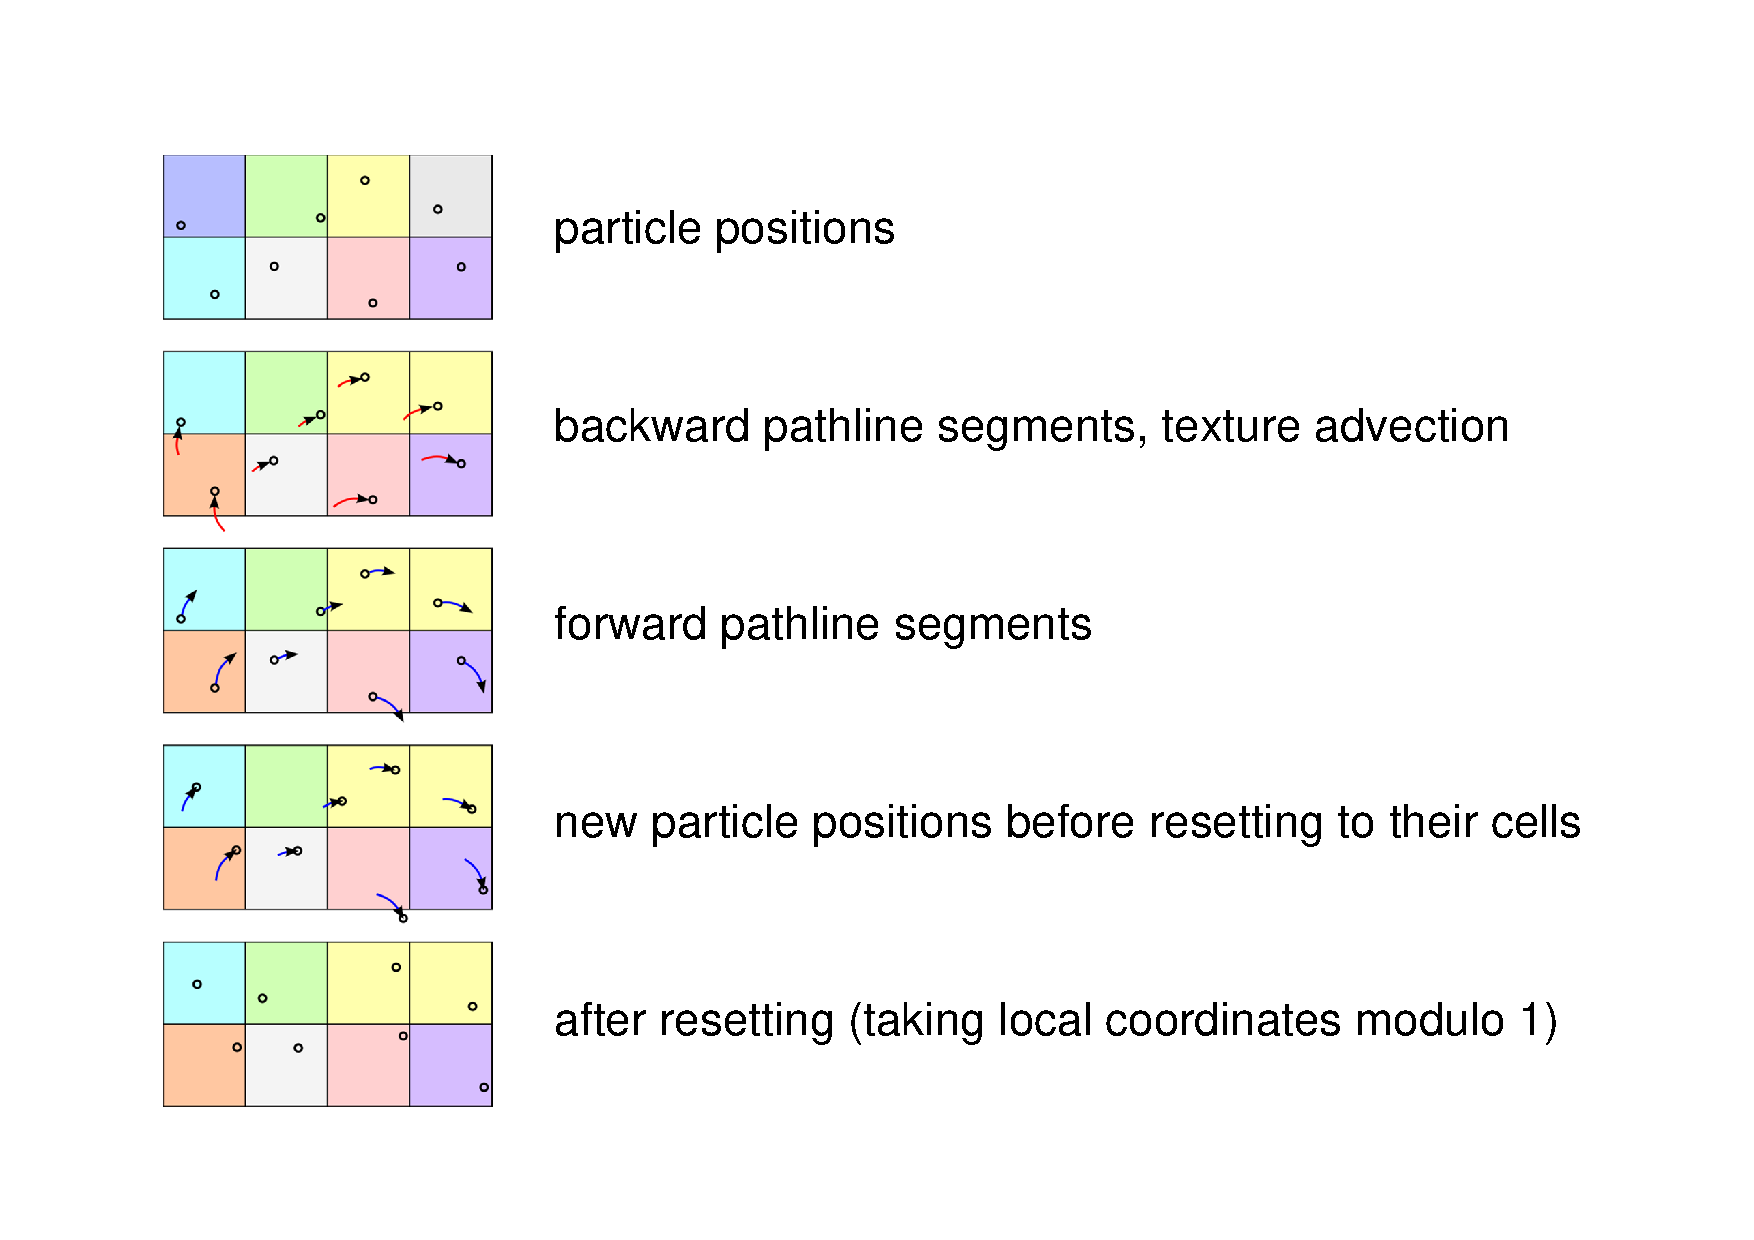
\includegraphics[width=0.8\textwidth]{img/06_eulerian_advection}
\end{figure}

\paragraph{Special choices made by LEA} $\ $ 
\begin{itemize}
    \item $1^{st}$ order integration
    \item Simplification: Forward segment = $-$backward segment
    
        Better: Backward segment = $-$previous forward semgent
    \item Add buffer cells at grid boundaries:
        \begin{itemize}
            \item Contain texture but no particles
            \item Allow texture advection at inflow boundaries
            \item Random texture is refreshed after each time step to avoid artefacts
        \end{itemize}
    \item Post-Processing: Apply a LIC filter to each image before outputting.
\end{itemize}
\paragraph{Interpolation}
Backward mapping scheme allows $2$ interpolation choices:
\begin{itemize}
    \item \emph{nearest-neighbour}
    \item Bilinear
\end{itemize}
LEA uses \emph{both}:
\begin{itemize}
    \item Nearest-neighbour is used for updating the \emph{stored} texture.
    \item Bilinear interpolation is used for \emph{displayed} texture
\end{itemize}

\paragraph{Noise injection} Backward mapping can have a duplication effect. Causes are:
\begin{itemize}
    \item Divergence of the vector field.
    \item Nearest-neighbour interpolation
\end{itemize}
\begin{figure}[H]
    \centering
    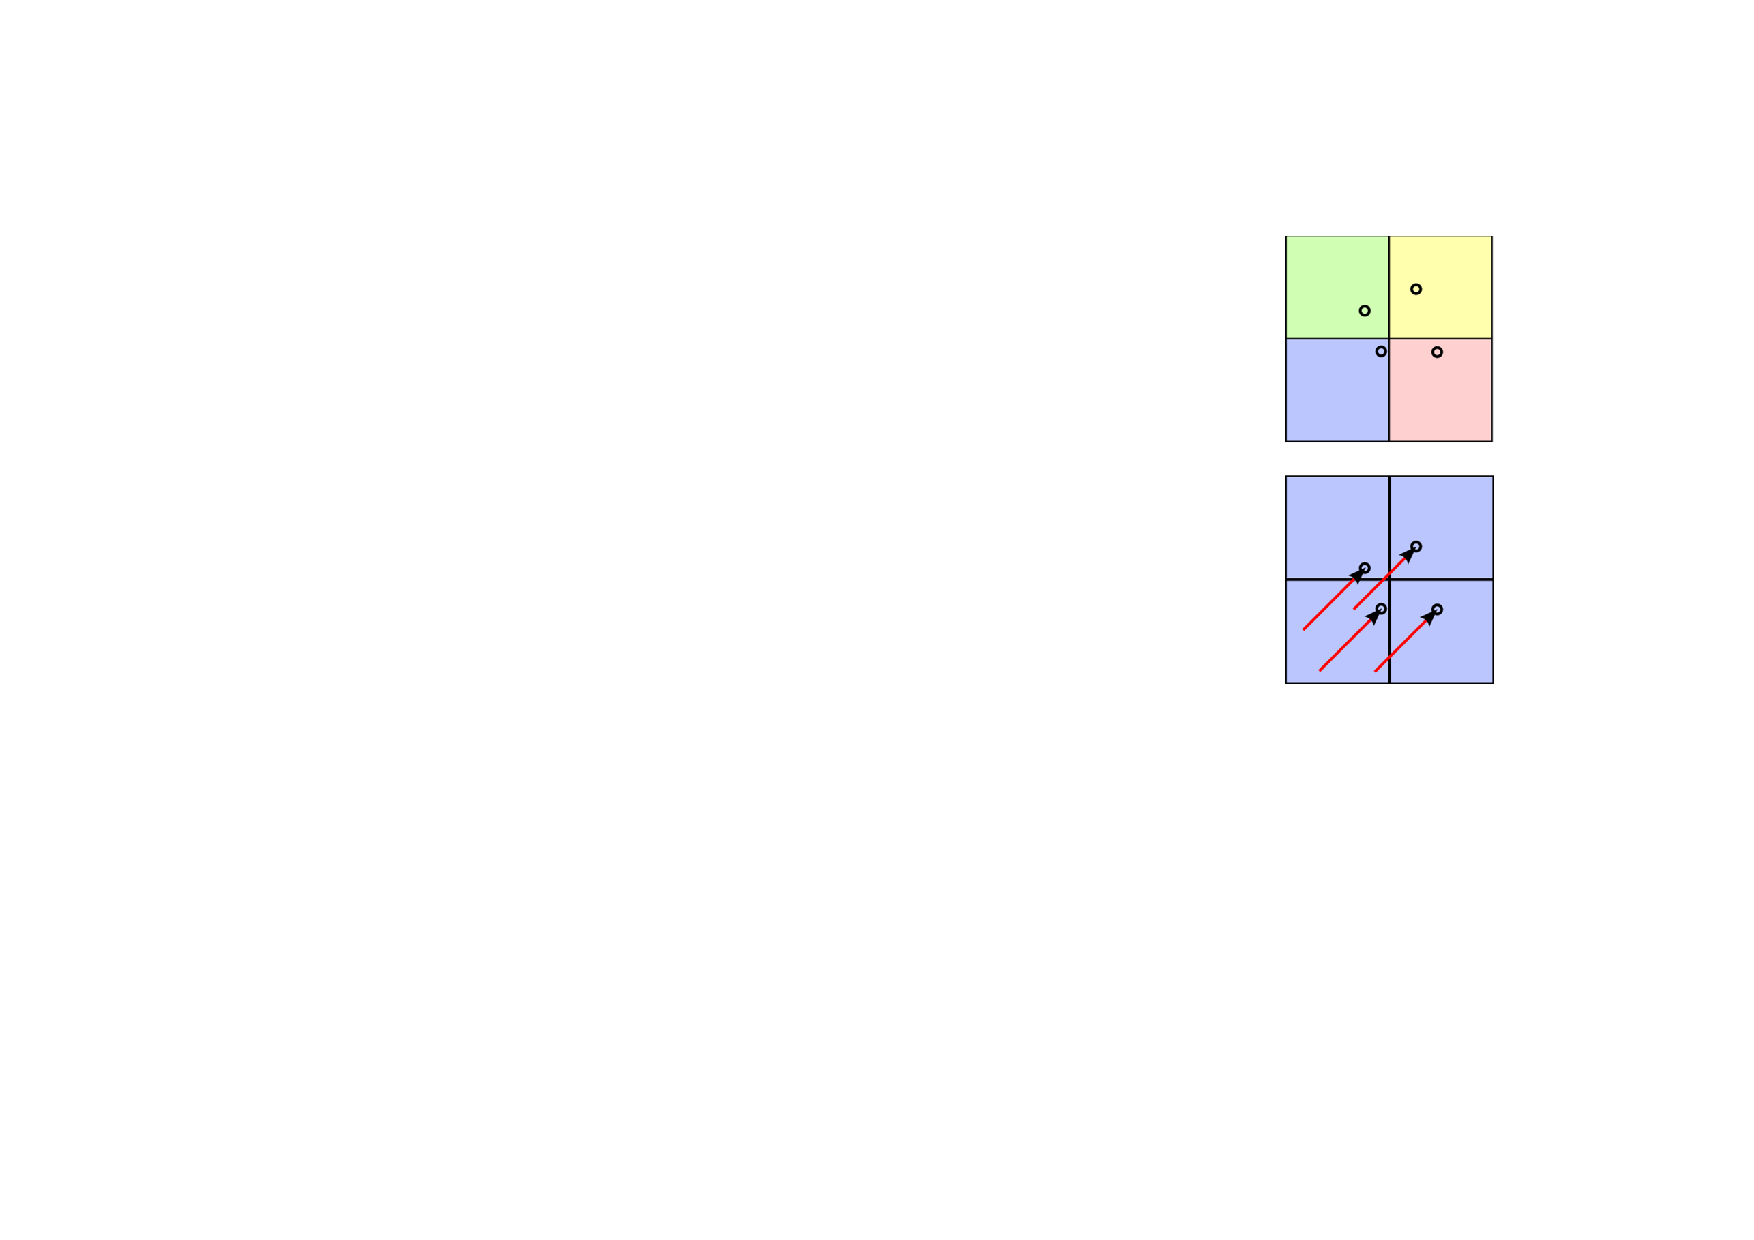
\includegraphics[width=0.4\textwidth]{img/06_noise_injection}
\end{figure}


Solution: \emph{Noise injection}: A small percentage of noise is added after each step. 

Trade-off: Keep high frequencies, but also temporal correlation.

\subsection{Image-Based Flow Visualisation}
IBFV algorithm (van Wijk 2002). Main idea:
\begin{itemize}
    \item Initialise a noise texture image.
    \item For each time step do:
        \begin{itemize}
            \item \emph{Advect nodes} of the texture image resulting in a warped grid.
            \item \emph{Render} the \emph{warped grid}, texture mapped.
            \item Resample the image to original mesh: 
            
                \emph{Read back} the rendered image to texture memory.
            \item Use as next texture image. 
        \end{itemize}
\end{itemize}
\begin{figure}[H]
    \centering
    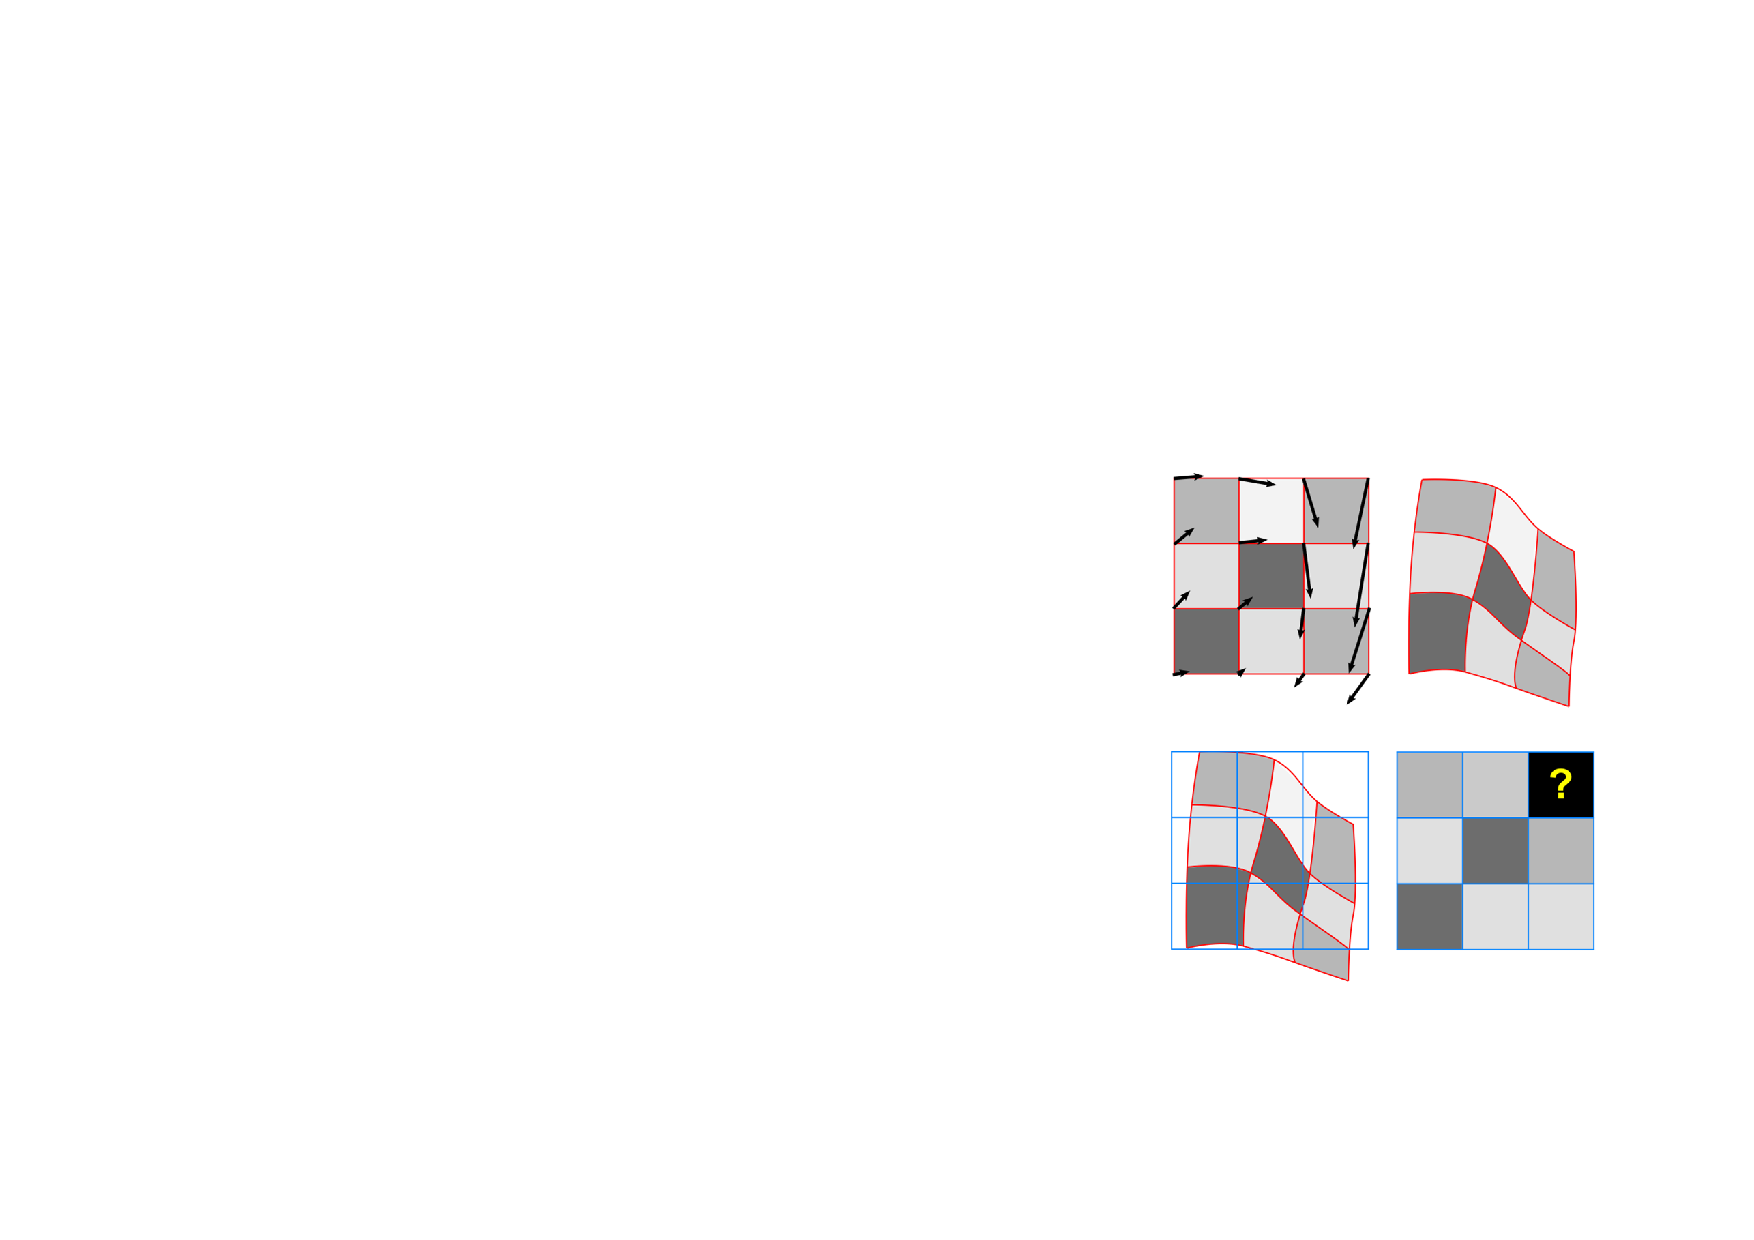
\includegraphics[width=0.4\textwidth]{img/06_ibfv}
\end{figure}


Detailed algorithm:
\begin{itemize}
    \item Initialise a noise texture image.
    \item For each time step do:
        \begin{itemize}
            \item Advect nodes of the texture image, resulting in a warped grid.
            \item Render the warped grid, texture mapped.
            \item \emph{Blend with noise image}.
            \item \emph{Apply dye injection}.
            \item Resample image to original mesh.
            \item Use as next texture image
            \item \emph{Draw overlaid graphics}
        \end{itemize}
\end{itemize}

\paragraph{Noise image}$\ $
\begin{description}
    \item \emph{Static} results in static image for steady flow
    \item \emph{Temporally coherent}, using \emph{spot noise} texture.
\end{description}

\paragraph{Boundary areas} For the boundary areas a special solution is needed. Simple solution: Don't clear the screen before redrawing. 

\paragraph{Comparison with LEA} IBFV is a much faster algorithm than LEA. The coherence is not as good.

\subsection{Texture advection in surfaces}
Texture advection on surfaces can be used for:
\begin{itemize}
    \item Boundary flow (wall shear stress)
    \item Flow on streamsurfaces
    \item Less meaningful: Project flow on other surfaces (isosurfaces)
\end{itemize}

Possible but expensive:
\begin{itemize}
    \item Work in object space
    \item Use 3D texture
\end{itemize}

Alternatives:
\begin{itemize}
    \item Work in image space:
        \begin{itemize}
            \item IBFV for surfaces (van Wijk)
            \item Image-space advection (Laramee)
        \end{itemize}
\end{itemize}

\subsection{IBFV for Surfaces}
Idea for IBFVS:
\begin{itemize}
    \item Use screen coordinates from previous rendering as texture coordinates.
    \item Advect in object space.
    
    I.e. Distort the surface mesh.
    \item Render the distorted mesh, keeping the texture coordinates
    \item Apply noise injection and blending
    \item Overlay the image
\end{itemize}

\subsection{Image-Space Advection}
Idea for ISA:
\begin{itemize}
    \item Project the velocity field to image space.
    \item Do IBFV within boundary silhouette.
    
    I.e. Advect rectangles.
    
    \item Apply noise injection and blending.
    \item Overlay image.
\end{itemize}

Comparison with IBFVS:
\begin{description}
\item Advantages:
    \begin{itemize}
        \item Projected velocity field simplifies advection
        \item No computation time is spent for hidden polygons and polygons smaller than a pixel
    \end{itemize}
\item Problems:
    \begin{itemize}
        \item Artificial continuity across interior silhouettes:
        
        ISA uses edge detection (depth discontinuities)
        
        \item The texture is not attached to the surface when the camera is moving.
    \end{itemize}

\end{description}


































\end{document}
